\PassOptionsToPackage{unicode=true}{hyperref} % options for packages loaded elsewhere
\PassOptionsToPackage{hyphens}{url}
%
\documentclass[]{book}
\usepackage{lmodern}
\usepackage{amssymb,amsmath}
\usepackage{ifxetex,ifluatex}
\usepackage{fixltx2e} % provides \textsubscript
\ifnum 0\ifxetex 1\fi\ifluatex 1\fi=0 % if pdftex
  \usepackage[T1]{fontenc}
  \usepackage[utf8]{inputenc}
  \usepackage{textcomp} % provides euro and other symbols
\else % if luatex or xelatex
  \usepackage{unicode-math}
  \defaultfontfeatures{Ligatures=TeX,Scale=MatchLowercase}
\fi
% use upquote if available, for straight quotes in verbatim environments
\IfFileExists{upquote.sty}{\usepackage{upquote}}{}
% use microtype if available
\IfFileExists{microtype.sty}{%
\usepackage[]{microtype}
\UseMicrotypeSet[protrusion]{basicmath} % disable protrusion for tt fonts
}{}
\IfFileExists{parskip.sty}{%
\usepackage{parskip}
}{% else
\setlength{\parindent}{0pt}
\setlength{\parskip}{6pt plus 2pt minus 1pt}
}
\usepackage{hyperref}
\hypersetup{
            pdftitle={An Introduction to R},
            pdfauthor={Vittorio Perduca (Université de Paris)},
            pdfborder={0 0 0},
            breaklinks=true}
\urlstyle{same}  % don't use monospace font for urls
\usepackage{color}
\usepackage{fancyvrb}
\newcommand{\VerbBar}{|}
\newcommand{\VERB}{\Verb[commandchars=\\\{\}]}
\DefineVerbatimEnvironment{Highlighting}{Verbatim}{commandchars=\\\{\}}
% Add ',fontsize=\small' for more characters per line
\usepackage{framed}
\definecolor{shadecolor}{RGB}{248,248,248}
\newenvironment{Shaded}{\begin{snugshade}}{\end{snugshade}}
\newcommand{\AlertTok}[1]{\textcolor[rgb]{0.94,0.16,0.16}{#1}}
\newcommand{\AnnotationTok}[1]{\textcolor[rgb]{0.56,0.35,0.01}{\textbf{\textit{#1}}}}
\newcommand{\AttributeTok}[1]{\textcolor[rgb]{0.77,0.63,0.00}{#1}}
\newcommand{\BaseNTok}[1]{\textcolor[rgb]{0.00,0.00,0.81}{#1}}
\newcommand{\BuiltInTok}[1]{#1}
\newcommand{\CharTok}[1]{\textcolor[rgb]{0.31,0.60,0.02}{#1}}
\newcommand{\CommentTok}[1]{\textcolor[rgb]{0.56,0.35,0.01}{\textit{#1}}}
\newcommand{\CommentVarTok}[1]{\textcolor[rgb]{0.56,0.35,0.01}{\textbf{\textit{#1}}}}
\newcommand{\ConstantTok}[1]{\textcolor[rgb]{0.00,0.00,0.00}{#1}}
\newcommand{\ControlFlowTok}[1]{\textcolor[rgb]{0.13,0.29,0.53}{\textbf{#1}}}
\newcommand{\DataTypeTok}[1]{\textcolor[rgb]{0.13,0.29,0.53}{#1}}
\newcommand{\DecValTok}[1]{\textcolor[rgb]{0.00,0.00,0.81}{#1}}
\newcommand{\DocumentationTok}[1]{\textcolor[rgb]{0.56,0.35,0.01}{\textbf{\textit{#1}}}}
\newcommand{\ErrorTok}[1]{\textcolor[rgb]{0.64,0.00,0.00}{\textbf{#1}}}
\newcommand{\ExtensionTok}[1]{#1}
\newcommand{\FloatTok}[1]{\textcolor[rgb]{0.00,0.00,0.81}{#1}}
\newcommand{\FunctionTok}[1]{\textcolor[rgb]{0.00,0.00,0.00}{#1}}
\newcommand{\ImportTok}[1]{#1}
\newcommand{\InformationTok}[1]{\textcolor[rgb]{0.56,0.35,0.01}{\textbf{\textit{#1}}}}
\newcommand{\KeywordTok}[1]{\textcolor[rgb]{0.13,0.29,0.53}{\textbf{#1}}}
\newcommand{\NormalTok}[1]{#1}
\newcommand{\OperatorTok}[1]{\textcolor[rgb]{0.81,0.36,0.00}{\textbf{#1}}}
\newcommand{\OtherTok}[1]{\textcolor[rgb]{0.56,0.35,0.01}{#1}}
\newcommand{\PreprocessorTok}[1]{\textcolor[rgb]{0.56,0.35,0.01}{\textit{#1}}}
\newcommand{\RegionMarkerTok}[1]{#1}
\newcommand{\SpecialCharTok}[1]{\textcolor[rgb]{0.00,0.00,0.00}{#1}}
\newcommand{\SpecialStringTok}[1]{\textcolor[rgb]{0.31,0.60,0.02}{#1}}
\newcommand{\StringTok}[1]{\textcolor[rgb]{0.31,0.60,0.02}{#1}}
\newcommand{\VariableTok}[1]{\textcolor[rgb]{0.00,0.00,0.00}{#1}}
\newcommand{\VerbatimStringTok}[1]{\textcolor[rgb]{0.31,0.60,0.02}{#1}}
\newcommand{\WarningTok}[1]{\textcolor[rgb]{0.56,0.35,0.01}{\textbf{\textit{#1}}}}
\usepackage{longtable,booktabs}
% Fix footnotes in tables (requires footnote package)
\IfFileExists{footnote.sty}{\usepackage{footnote}\makesavenoteenv{longtable}}{}
\usepackage{graphicx,grffile}
\makeatletter
\def\maxwidth{\ifdim\Gin@nat@width>\linewidth\linewidth\else\Gin@nat@width\fi}
\def\maxheight{\ifdim\Gin@nat@height>\textheight\textheight\else\Gin@nat@height\fi}
\makeatother
% Scale images if necessary, so that they will not overflow the page
% margins by default, and it is still possible to overwrite the defaults
% using explicit options in \includegraphics[width, height, ...]{}
\setkeys{Gin}{width=\maxwidth,height=\maxheight,keepaspectratio}
\setlength{\emergencystretch}{3em}  % prevent overfull lines
\providecommand{\tightlist}{%
  \setlength{\itemsep}{0pt}\setlength{\parskip}{0pt}}
\setcounter{secnumdepth}{5}
% Redefines (sub)paragraphs to behave more like sections
\ifx\paragraph\undefined\else
\let\oldparagraph\paragraph
\renewcommand{\paragraph}[1]{\oldparagraph{#1}\mbox{}}
\fi
\ifx\subparagraph\undefined\else
\let\oldsubparagraph\subparagraph
\renewcommand{\subparagraph}[1]{\oldsubparagraph{#1}\mbox{}}
\fi

% set default figure placement to htbp
\makeatletter
\def\fps@figure{htbp}
\makeatother

\usepackage{booktabs}
\usepackage[]{natbib}
\bibliographystyle{apalike}

\title{An Introduction to R}
\author{Vittorio Perduca (Université de Paris)}
\date{September 2020}

\begin{document}
\maketitle

{
\setcounter{tocdepth}{1}
\tableofcontents
}
\hypertarget{welcome}{%
\chapter{Welcome}\label{welcome}}

This document is a tutorial for self-learning the basic use of \texttt{R}. It was prepared for the students enrolled in the first year of the \href{https://www.cri-paris.org/en/education\#04._aire-master}{AIRE Life Sciences Master Program} of the Centre de Recherche Interdisciplinaire at the Université de Paris.

\begin{center}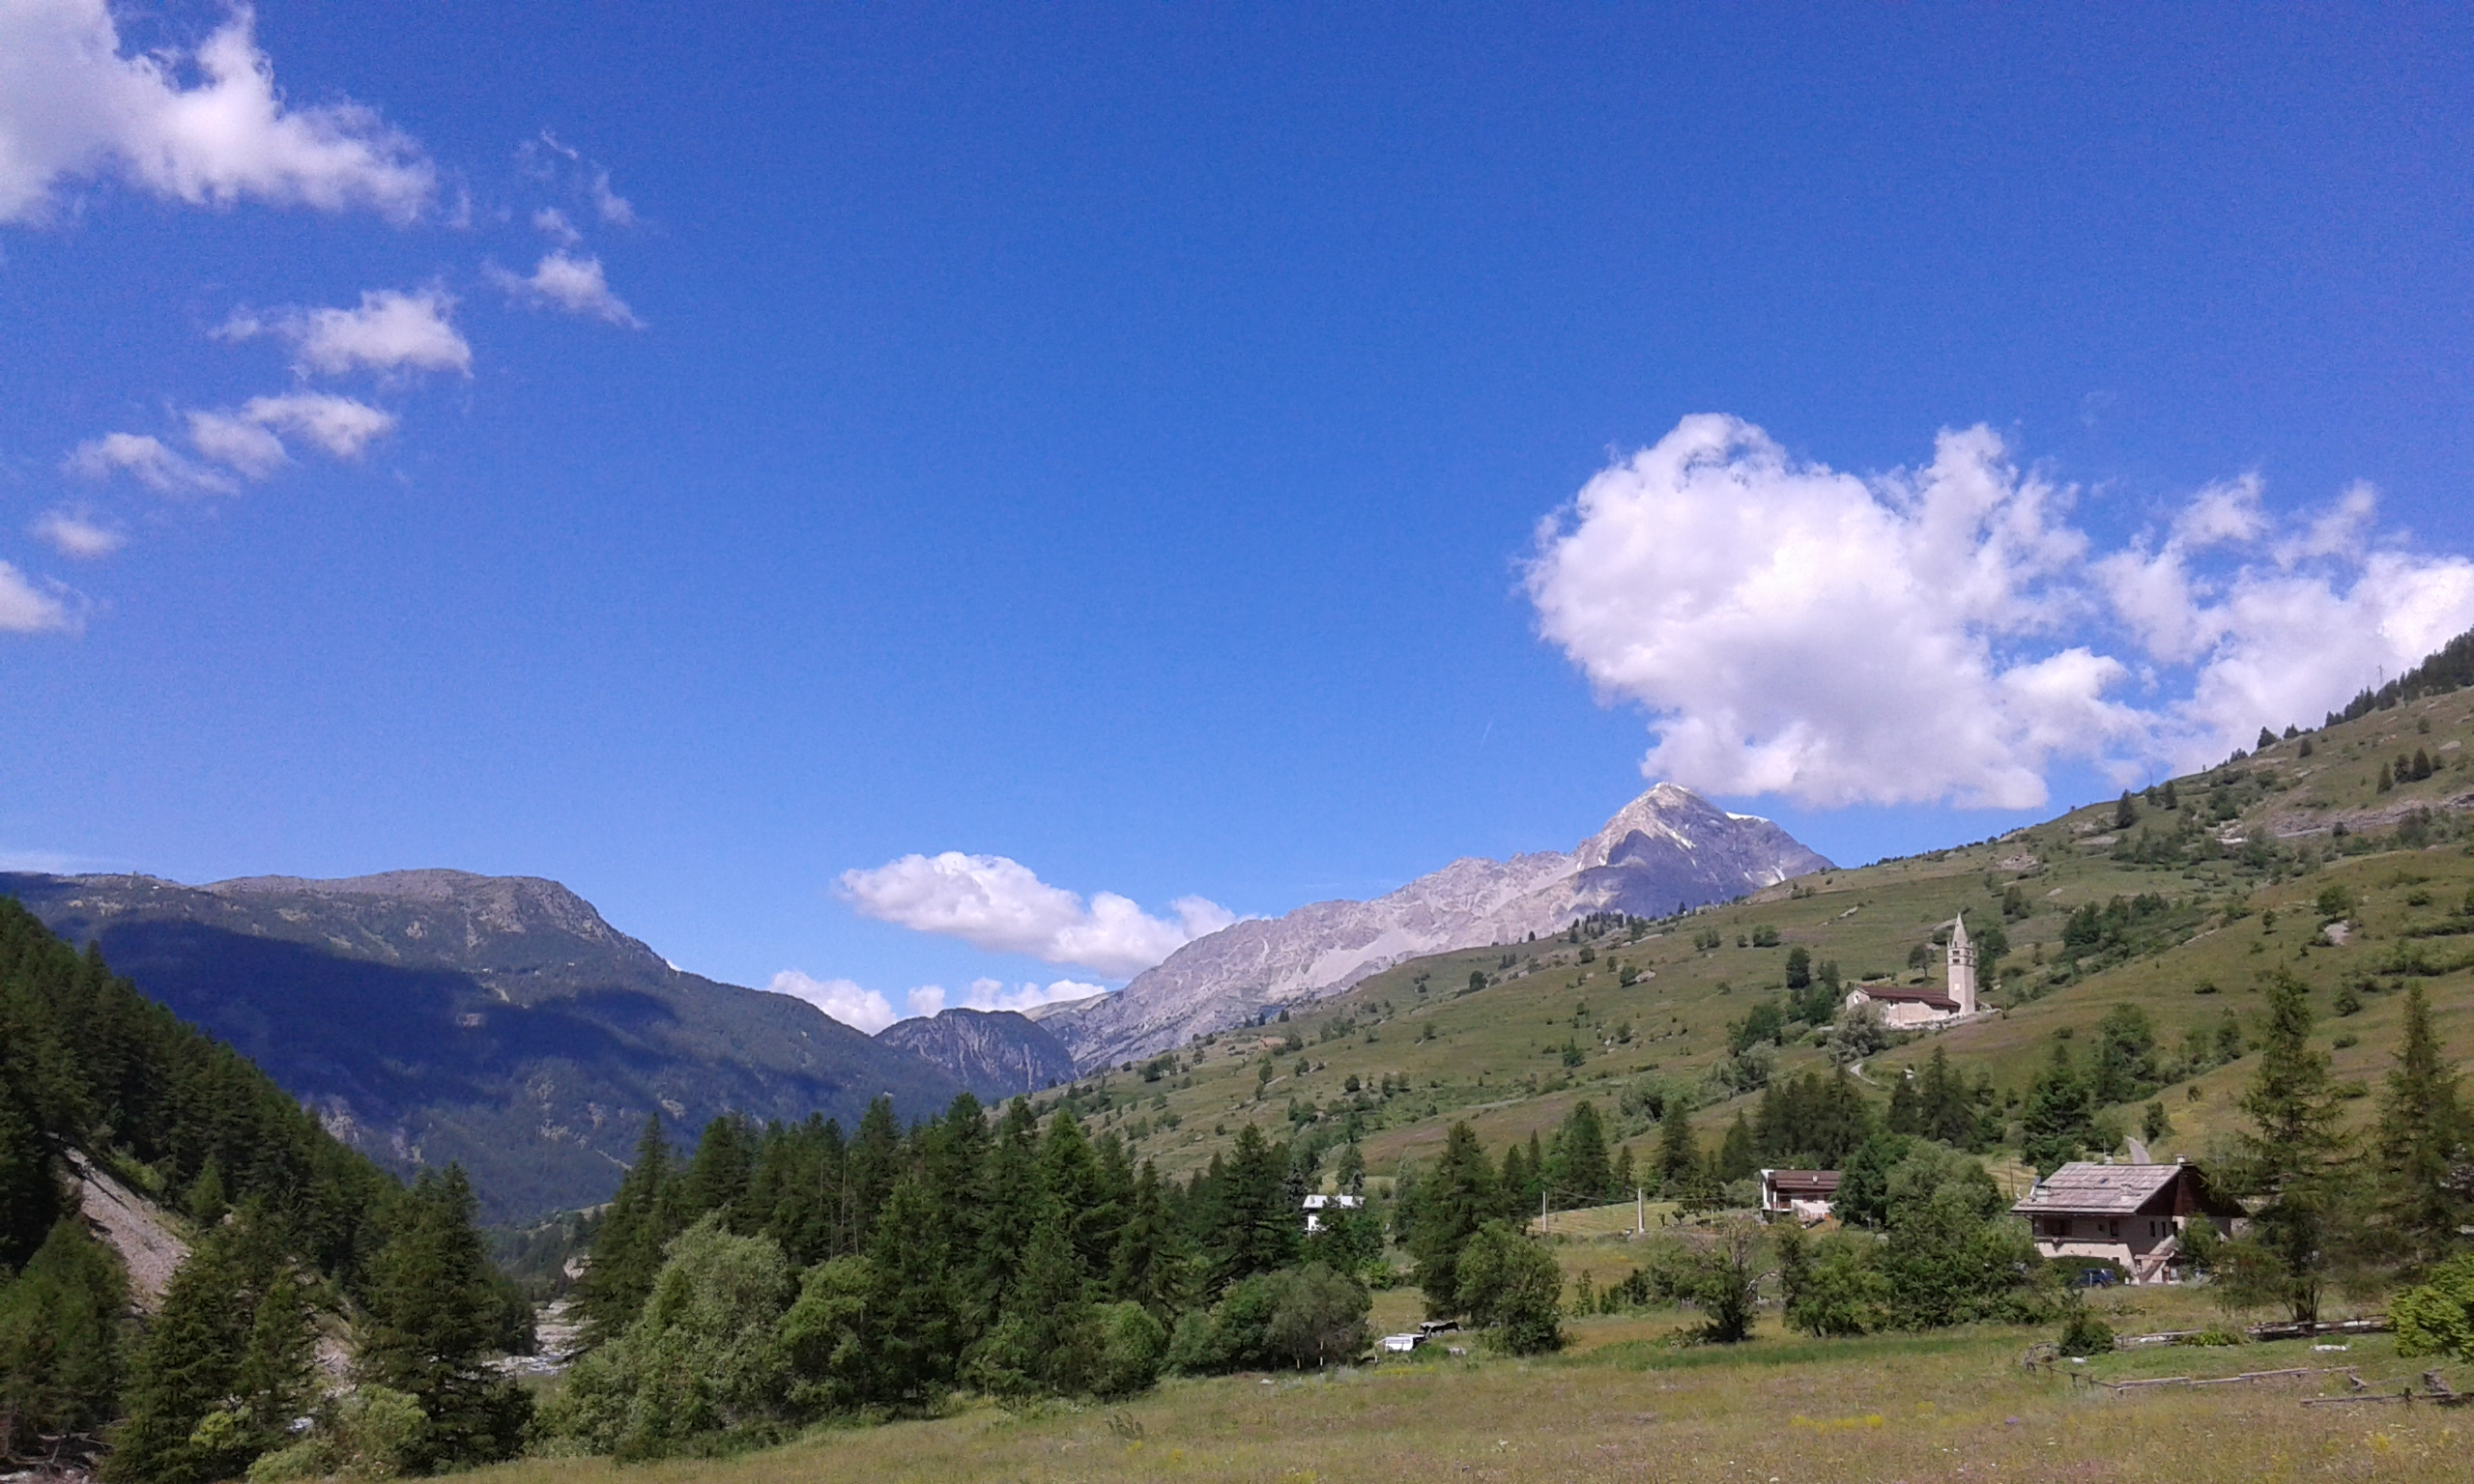
\includegraphics[width=0.9\linewidth]{images/san-restituto} \end{center}

This document was written with the \texttt{R} package \texttt{bookdown} \citep{R-bookdown}, \citep{bookdown2016} and is under continuous development, please report any issues to \texttt{vittorio.perduca\ at\ u-paris.fr}. This work is licensed under \href{https://creativecommons.org/licenses/by-nc/4.0/}{CC BY-NC 4.0}.

\hypertarget{introduction}{%
\chapter{Introduction}\label{introduction}}

\texttt{R} is a statistical language developed from the 1990s at the University of Auckland, New Zealand. Its main implementation is the open source software (free and modifiable) \texttt{R}. \texttt{R} is normally used from the graphical user interface (GUI) and development interface RStudio.

\texttt{R} is an \href{http://www.france-ioi.org/algo/course.php?idChapter=561\&idCourse=2368}{interpreted language} (like\texttt{Python}) that we use from the command line:

\begin{Shaded}
\begin{Highlighting}[]
\KeywordTok{print}\NormalTok{ (}\StringTok{'Hello world!'}\NormalTok{)}
\end{Highlighting}
\end{Shaded}

\begin{verbatim}
## [1] "Hello world!"
\end{verbatim}

Alternatively, you can run a script, that is a series of commands found in a file with the extension \texttt{.R}.

The \texttt{R} user community is very active in the scientific world (statistics, data science, bioinformatics, social sciences, \ldots{}) and more and more in companies. One of the advantages of \texttt{R} is the wealth of \emph{packages} developed by users and developers that can be installed to increase its capabilities in many areas of statistics.

In addition, \texttt{R} has a very complete documentation. You can access help by typing \texttt{?} followed by the \emph{function} you are interested in:

\begin{Shaded}
\begin{Highlighting}[]
\NormalTok{? rnorm}
\end{Highlighting}
\end{Shaded}

You can also find a lot of information on the web: by searching on Google for a problem related to an \texttt{R} task, you almost always find an answer (often in threads opened on \href{https:\%20//\%20stats\%20.stackexchange.com\%20/}{Cross Validated}).

\hypertarget{how-to-use-this-document}{%
\section{How to use this document}\label{how-to-use-this-document}}

Although basic objects and commands are covered, this introduction is not a complete reference to the \texttt{R} language, so you will have to use the help and search for information on the web. Before moving on to the exercises at the end of each chapter, you are encouraged to type the commands and understand the result: the best way to learn a language is to write and debug lots of lines of code!

\hypertarget{useful-references}{%
\section{Useful references}\label{useful-references}}

A complete reference to \texttt{R} is the official introduction that can be found on the CRAN website: \url{https://cran.r-project.org/doc/manuals/R-intro.html}. For French readers, an excellent reference is Vincent Goulet's book \emph{Introduction à la programmation R}, which can be downloaded at \url{https://cran.r-project.org/doc/contrib/Goulet_introduction_programmation_R.pdf}

\hypertarget{installing-r-and-rstudio}{%
\section{Installing R and Rstudio}\label{installing-r-and-rstudio}}

\begin{enumerate}
\def\labelenumi{\arabic{enumi}.}
\tightlist
\item
  Download the \texttt{R} distribution that is appropriate for your machine from \url{https://cran.r-project.org/} and install it by double-clicking on the installation file.
\item
  Dowanload and install RStudio Desktop from \url{https://rstudio.com/products/rstudio/download/}.
\end{enumerate}

\hypertarget{getting-started-with-rstudio}{%
\section{Getting started with RStudio}\label{getting-started-with-rstudio}}

The RStudio workspace is generally divided into four pans: starting from the top left and going clockwise we find:

\begin{enumerate}
\def\labelenumi{\arabic{enumi}.}
\tightlist
\item
  a script editor
\item
  the environment listing the variables in memory and the history of commands that were executed
\item
  a window for graphical outputs, the help, and the file and package managers.
\item
  the \texttt{R} console, ie the command line.
\end{enumerate}

Typically we type the code in the editor and then run it in the console. To do this we place the cursor in the line we want to execute and we send the command to the console using the combination \texttt{cmd\ Return} in macOS and\texttt{ctrl\ Return} under Linux and Windows.

\hypertarget{packages}{%
\section{Packages}\label{packages}}

To install a package from the console:

\begin{Shaded}
\begin{Highlighting}[]
\KeywordTok{install.packages}\NormalTok{(}\StringTok{"dplyr"}\NormalTok{)}
\CommentTok{# download and install the dplyr package used for data manipulation}
\end{Highlighting}
\end{Shaded}

Once a package is installed, it will have to be loaded into memory each time a new session is opened:

\begin{Shaded}
\begin{Highlighting}[]
\KeywordTok{library}\NormalTok{(dplyr) }\CommentTok{# quotes are not needed here}
\CommentTok{# require(dplyr) # equivalent function}
\end{Highlighting}
\end{Shaded}

\hypertarget{language-basics}{%
\chapter{Language basics}\label{language-basics}}

\hypertarget{assignments-arithmetic-operations}{%
\section{Assignments, arithmetic operations}\label{assignments-arithmetic-operations}}

There are two types of \texttt{R} commands: expressions and assignments.

\textbf{Expression}

\begin{Shaded}
\begin{Highlighting}[]
\KeywordTok{cos}\NormalTok{(pi)}
\end{Highlighting}
\end{Shaded}

\begin{verbatim}
## [1] -1
\end{verbatim}

\textbf{Assignments and expressions}

\begin{Shaded}
\begin{Highlighting}[]
\NormalTok{x <-}\StringTok{ }\DecValTok{1} \OperatorTok{+}\StringTok{ }\DecValTok{2} \CommentTok{# or x = 1 + 2}
\NormalTok{x}
\end{Highlighting}
\end{Shaded}

\begin{verbatim}
## [1] 3
\end{verbatim}

\begin{Shaded}
\begin{Highlighting}[]
\NormalTok{y =}\StringTok{ }\DecValTok{4}
\NormalTok{x }\OperatorTok{==}\StringTok{ }\NormalTok{y}
\end{Highlighting}
\end{Shaded}

\begin{verbatim}
## [1] FALSE
\end{verbatim}

Using \texttt{;} we can type two commands on the same line before executing them:

\begin{Shaded}
\begin{Highlighting}[]
\NormalTok{e <-}\StringTok{ }\KeywordTok{exp}\NormalTok{ (}\DecValTok{1}\NormalTok{); }\KeywordTok{log}\NormalTok{ (e)}
\end{Highlighting}
\end{Shaded}

\begin{verbatim}
## [1] 1
\end{verbatim}

Some examples of arithmetic and Boolean operators:

\begin{Shaded}
\begin{Highlighting}[]
\DecValTok{3}\OperatorTok{*}\DecValTok{4}
\end{Highlighting}
\end{Shaded}

\begin{verbatim}
## [1] 12
\end{verbatim}

\begin{Shaded}
\begin{Highlighting}[]
\DecValTok{12}\OperatorTok{/}\DecValTok{3}
\end{Highlighting}
\end{Shaded}

\begin{verbatim}
## [1] 4
\end{verbatim}

\begin{Shaded}
\begin{Highlighting}[]
\DecValTok{2}\OperatorTok{^}\DecValTok{3}
\end{Highlighting}
\end{Shaded}

\begin{verbatim}
## [1] 8
\end{verbatim}

\begin{Shaded}
\begin{Highlighting}[]
\KeywordTok{sqrt}\NormalTok{ (}\DecValTok{16}\NormalTok{)}
\end{Highlighting}
\end{Shaded}

\begin{verbatim}
## [1] 4
\end{verbatim}

\begin{Shaded}
\begin{Highlighting}[]
\DecValTok{1} \OperatorTok{==}\StringTok{ }\DecValTok{2}
\end{Highlighting}
\end{Shaded}

\begin{verbatim}
## [1] FALSE
\end{verbatim}

\begin{Shaded}
\begin{Highlighting}[]
\DecValTok{1}\OperatorTok{!=}\StringTok{ }\DecValTok{1}
\end{Highlighting}
\end{Shaded}

\begin{verbatim}
## [1] FALSE
\end{verbatim}

\begin{Shaded}
\begin{Highlighting}[]
\OtherTok{FALSE} \OperatorTok{&}\StringTok{ }\OtherTok{TRUE} \CommentTok{# and}
\end{Highlighting}
\end{Shaded}

\begin{verbatim}
## [1] FALSE
\end{verbatim}

\begin{Shaded}
\begin{Highlighting}[]
\OtherTok{FALSE} \OperatorTok{|}\StringTok{ }\OtherTok{TRUE} \CommentTok{# or}
\end{Highlighting}
\end{Shaded}

\begin{verbatim}
## [1] TRUE
\end{verbatim}

\hypertarget{mode-length-and-class}{%
\section{Mode, length and class}\label{mode-length-and-class}}

In R, everything is an \emph{object}. The \emph{mode} specifies what an object can contain. The main modes are:

\begin{itemize}
\tightlist
\item
  \texttt{numeric}: real numbers
\item
  \texttt{character}: character strings
\item
  \texttt{logical}: logical values true / false
\item
  \texttt{list}: list, collection of objects
\item
  \texttt{function}: function
\end{itemize}

\texttt{numeric},\texttt{character}, and \texttt{logical} objects are \emph{simple} objects that can contain data of only one type. On the contrary, \texttt{list} mobjects are special objects that can contain other objects.

You can access the mode of an object with the \texttt{mode\ ()} function:

\begin{Shaded}
\begin{Highlighting}[]
\NormalTok{age =}\StringTok{ }\KeywordTok{c}\NormalTok{(}\DecValTok{33}\NormalTok{,}\DecValTok{28}\NormalTok{, }\DecValTok{33}\NormalTok{) }\CommentTok{# The concatenation function c() allows to create vectors}
\KeywordTok{mode}\NormalTok{(age)}
\end{Highlighting}
\end{Shaded}

\begin{verbatim}
## [1] "numeric"
\end{verbatim}

\begin{Shaded}
\begin{Highlighting}[]
\NormalTok{names <-}\StringTok{ }\KeywordTok{c}\NormalTok{(}\StringTok{'Daniel'}\NormalTok{, }\StringTok{'Jehanne'}\NormalTok{, }\StringTok{'Romain'}\NormalTok{)}
\KeywordTok{mode}\NormalTok{(names)}
\end{Highlighting}
\end{Shaded}

\begin{verbatim}
## [1] "character"
\end{verbatim}

\begin{Shaded}
\begin{Highlighting}[]
\NormalTok{my.list <-}\StringTok{ }\KeywordTok{list}\NormalTok{(}\DataTypeTok{Names =}\NormalTok{ names, }\DataTypeTok{Age =}\NormalTok{ age)}
\KeywordTok{mode}\NormalTok{(my.list)}
\end{Highlighting}
\end{Shaded}

\begin{verbatim}
## [1] "list"
\end{verbatim}

\begin{Shaded}
\begin{Highlighting}[]
\KeywordTok{mode}\NormalTok{(}\KeywordTok{is.integer}\NormalTok{(pi))}
\end{Highlighting}
\end{Shaded}

\begin{verbatim}
## [1] "logical"
\end{verbatim}

\begin{Shaded}
\begin{Highlighting}[]
\NormalTok{mode}
\end{Highlighting}
\end{Shaded}

\begin{verbatim}
## function (x) 
## {
##     if (is.expression(x)) 
##         return("expression")
##     if (is.call(x)) 
##         return(switch(deparse(x[[1L]])[1L], `(` = "(", "call"))
##     if (is.name(x)) 
##         "name"
##     else switch(tx <- typeof(x), double = , integer = "numeric", 
##         closure = , builtin = , special = "function", tx)
## }
## <bytecode: 0x7fae3e7a0e90>
## <environment: namespace:base>
\end{verbatim}

Besides the mode, an object also has a \emph{length}, defined as the number of elements it contains:

\begin{Shaded}
\begin{Highlighting}[]
\KeywordTok{length}\NormalTok{(age)}
\end{Highlighting}
\end{Shaded}

\begin{verbatim}
## [1] 3
\end{verbatim}

\begin{Shaded}
\begin{Highlighting}[]
\KeywordTok{length}\NormalTok{(names)}
\end{Highlighting}
\end{Shaded}

\begin{verbatim}
## [1] 3
\end{verbatim}

\begin{Shaded}
\begin{Highlighting}[]
\KeywordTok{length}\NormalTok{(my.list)}
\end{Highlighting}
\end{Shaded}

\begin{verbatim}
## [1] 2
\end{verbatim}

The \emph{class} of an object specifies its behavior and therefore its way of interacting with operations and functions. An important example are \emph{data frames}: special lists whose elements all have the same length. The class of a data frame is different from that of generic lists and data frames have an indexing system that does not exist for other lists:

\begin{Shaded}
\begin{Highlighting}[]
\KeywordTok{class}\NormalTok{(my.list)}
\end{Highlighting}
\end{Shaded}

\begin{verbatim}
## [1] "list"
\end{verbatim}

\begin{Shaded}
\begin{Highlighting}[]
\NormalTok{my.data.frame =}\StringTok{ }\KeywordTok{data.frame}\NormalTok{(names, age)}
\KeywordTok{mode}\NormalTok{(my.data.frame)}
\end{Highlighting}
\end{Shaded}

\begin{verbatim}
## [1] "list"
\end{verbatim}

\begin{Shaded}
\begin{Highlighting}[]
\KeywordTok{class}\NormalTok{(my.data.frame)}
\end{Highlighting}
\end{Shaded}

\begin{verbatim}
## [1] "data.frame"
\end{verbatim}

\begin{Shaded}
\begin{Highlighting}[]
\NormalTok{my.data.frame[}\DecValTok{1}\NormalTok{,}\DecValTok{2}\NormalTok{] }\CommentTok{# to extract the 1st element from the 2nd "column"}
\end{Highlighting}
\end{Shaded}

\begin{verbatim}
## [1] 33
\end{verbatim}

\begin{Shaded}
\begin{Highlighting}[]
\CommentTok{# Try the following command:}
\CommentTok{# my.list[1,2]}
\end{Highlighting}
\end{Shaded}

A special object is the missing value \texttt{NA}. By default, its mode is \texttt{logical}, however\texttt{NA} is neither \texttt{TRUE} nor\texttt{FALSE}. To test if a value is missing we will use the \texttt{is.na\ ()} function:

\begin{Shaded}
\begin{Highlighting}[]
\OtherTok{NA} \OperatorTok{==}\StringTok{ }\OtherTok{NA} \CommentTok{# not what we want}
\end{Highlighting}
\end{Shaded}

\begin{verbatim}
## [1] NA
\end{verbatim}

\begin{Shaded}
\begin{Highlighting}[]
\KeywordTok{is.na}\NormalTok{(}\OtherTok{NA}\NormalTok{)}
\end{Highlighting}
\end{Shaded}

\begin{verbatim}
## [1] TRUE
\end{verbatim}

\begin{Shaded}
\begin{Highlighting}[]
\KeywordTok{is.na}\NormalTok{(}\KeywordTok{mean}\NormalTok{(}\KeywordTok{c}\NormalTok{(}\DecValTok{1}\NormalTok{,}\DecValTok{4}\NormalTok{, }\OtherTok{NA}\NormalTok{)))}
\end{Highlighting}
\end{Shaded}

\begin{verbatim}
## [1] TRUE
\end{verbatim}

\hypertarget{vectors-matrices-and-functions}{%
\chapter{Vectors, matrices and functions}\label{vectors-matrices-and-functions}}

\hypertarget{vectors}{%
\section{Vectors}\label{vectors}}

The \texttt{R} basic object is the \emph{vector} (a scalar is considered as a vector of length one). The most used function to create a vector is the concatenation:

\begin{Shaded}
\begin{Highlighting}[]
\NormalTok{price <-}\StringTok{ }\KeywordTok{c}\NormalTok{(}\DecValTok{150}\NormalTok{, }\DecValTok{162}\NormalTok{, }\DecValTok{155}\NormalTok{, }\DecValTok{157}\NormalTok{); price}
\end{Highlighting}
\end{Shaded}

\begin{verbatim}
## [1] 150 162 155 157
\end{verbatim}

\textbf{Indexing} is done through brackets:

\begin{Shaded}
\begin{Highlighting}[]
\NormalTok{price[}\DecValTok{1}\NormalTok{] }\CommentTok{# Unlike in Python, the first index is always 1!!}
\end{Highlighting}
\end{Shaded}

\begin{verbatim}
## [1] 150
\end{verbatim}

\begin{Shaded}
\begin{Highlighting}[]
\NormalTok{price[}\KeywordTok{c}\NormalTok{(}\FloatTok{1.3}\NormalTok{)]}
\end{Highlighting}
\end{Shaded}

\begin{verbatim}
## [1] 150
\end{verbatim}

\begin{Shaded}
\begin{Highlighting}[]
\NormalTok{price[}\OperatorTok{-}\NormalTok{(}\DecValTok{1}\OperatorTok{:}\DecValTok{2}\NormalTok{)] }\CommentTok{# to extract all elements except the 1st and 2nd}
\end{Highlighting}
\end{Shaded}

\begin{verbatim}
## [1] 155 157
\end{verbatim}

One can also use a boolean indexing vector, the extracted elements are obviously those corresponding to the \texttt{TRUE} values. For example to extract prices greater than 156:

\begin{Shaded}
\begin{Highlighting}[]
\NormalTok{price }\OperatorTok{>}\StringTok{ }\DecValTok{156} \CommentTok{# the boolean vector}
\end{Highlighting}
\end{Shaded}

\begin{verbatim}
## [1] FALSE  TRUE FALSE  TRUE
\end{verbatim}

\begin{Shaded}
\begin{Highlighting}[]
\NormalTok{price[price }\OperatorTok{>}\StringTok{ }\DecValTok{156}\NormalTok{]}
\end{Highlighting}
\end{Shaded}

\begin{verbatim}
## [1] 162 157
\end{verbatim}

An alternative is given by the \texttt{which\ ()} function which returns the indices whose elements satisfy a logical condition:

\begin{Shaded}
\begin{Highlighting}[]
\KeywordTok{which}\NormalTok{(price }\OperatorTok{>}\StringTok{ }\DecValTok{155}\NormalTok{)}
\end{Highlighting}
\end{Shaded}

\begin{verbatim}
## [1] 2 4
\end{verbatim}

\begin{Shaded}
\begin{Highlighting}[]
\NormalTok{price[}\KeywordTok{which}\NormalTok{(price }\OperatorTok{>}\StringTok{ }\DecValTok{156}\NormalTok{)]}
\end{Highlighting}
\end{Shaded}

\begin{verbatim}
## [1] 162 157
\end{verbatim}

You can use the indexing to change an element:

\begin{Shaded}
\begin{Highlighting}[]
\NormalTok{price [}\DecValTok{1}\NormalTok{] <-}\StringTok{ }\DecValTok{0}\NormalTok{; price}
\end{Highlighting}
\end{Shaded}

\begin{verbatim}
## [1]   0 162 155 157
\end{verbatim}

It is possible to give labels to the elements of a vector and extract elements based on them:

\begin{Shaded}
\begin{Highlighting}[]
\KeywordTok{names}\NormalTok{(price) }
\end{Highlighting}
\end{Shaded}

\begin{verbatim}
## NULL
\end{verbatim}

\begin{Shaded}
\begin{Highlighting}[]
\CommentTok{# NULL is a special object with NULL mode that reads "no container"}
\KeywordTok{names}\NormalTok{(price) <-}\StringTok{ }\KeywordTok{c}\NormalTok{(}\StringTok{'model.1'}\NormalTok{, }\StringTok{'model.2'}\NormalTok{, }\StringTok{'model.3'}\NormalTok{, }\StringTok{'model.4'}\NormalTok{)}
\NormalTok{price}
\end{Highlighting}
\end{Shaded}

\begin{verbatim}
## model.1 model.2 model.3 model.4 
##       0     162     155     157
\end{verbatim}

\begin{Shaded}
\begin{Highlighting}[]
\NormalTok{price[}\StringTok{'model.3'}\NormalTok{]}
\end{Highlighting}
\end{Shaded}

\begin{verbatim}
## model.3 
##     155
\end{verbatim}

In a vector, all the elements must have the same mode:

\begin{Shaded}
\begin{Highlighting}[]
\NormalTok{x <-}\StringTok{ }\KeywordTok{c}\NormalTok{(}\DecValTok{1}\NormalTok{,}\DecValTok{2}\NormalTok{, }\StringTok{'a'}\NormalTok{, }\StringTok{'b'}\NormalTok{); x}
\end{Highlighting}
\end{Shaded}

\begin{verbatim}
## [1] "1" "2" "a" "b"
\end{verbatim}

\begin{Shaded}
\begin{Highlighting}[]
\KeywordTok{mode}\NormalTok{(x)}
\end{Highlighting}
\end{Shaded}

\begin{verbatim}
## [1] "character"
\end{verbatim}

To generate the vector of the first \(n\) integers we use the syntax \texttt{1:n}

\begin{Shaded}
\begin{Highlighting}[]
\DecValTok{1}\OperatorTok{:}\DecValTok{10}
\end{Highlighting}
\end{Shaded}

\begin{verbatim}
##  [1]  1  2  3  4  5  6  7  8  9 10
\end{verbatim}

\begin{Shaded}
\begin{Highlighting}[]
\DecValTok{2}\OperatorTok{:}\DecValTok{6}
\end{Highlighting}
\end{Shaded}

\begin{verbatim}
## [1] 2 3 4 5 6
\end{verbatim}

To generate more general sequences we use the \texttt{seq()} function:

\begin{Shaded}
\begin{Highlighting}[]
\KeywordTok{seq}\NormalTok{(}\DataTypeTok{from =} \DecValTok{2}\NormalTok{, }\DataTypeTok{to =} \DecValTok{20}\NormalTok{, }\DataTypeTok{by =} \DecValTok{2}\NormalTok{) }\CommentTok{# or more simply seq(2,20,2)}
\end{Highlighting}
\end{Shaded}

\begin{verbatim}
##  [1]  2  4  6  8 10 12 14 16 18 20
\end{verbatim}

We can create a vector of repeated elements with \texttt{rep()}:

\begin{Shaded}
\begin{Highlighting}[]
\KeywordTok{rep}\NormalTok{(}\DecValTok{1}\NormalTok{, }\DataTypeTok{len =} \DecValTok{3}\NormalTok{) }\CommentTok{# same thing as rep (1,3)}
\end{Highlighting}
\end{Shaded}

\begin{verbatim}
## [1] 1 1 1
\end{verbatim}

\begin{Shaded}
\begin{Highlighting}[]
\KeywordTok{rep}\NormalTok{(}\OtherTok{NA}\NormalTok{, }\DecValTok{4}\NormalTok{)}
\end{Highlighting}
\end{Shaded}

\begin{verbatim}
## [1] NA NA NA NA
\end{verbatim}

\hypertarget{matrices}{%
\section{Matrices}\label{matrices}}

A matrix is a vector with a \texttt{dim} attribute of length two. All the elements of a matrix therefore have the same mode. To create a matrix:

\begin{Shaded}
\begin{Highlighting}[]
\NormalTok{M <-}\StringTok{ }\KeywordTok{matrix}\NormalTok{(}\DecValTok{2}\OperatorTok{:}\DecValTok{7}\NormalTok{, }\DataTypeTok{nrow =} \DecValTok{2}\NormalTok{, }\DataTypeTok{ncol =} \DecValTok{3}\NormalTok{); M}
\end{Highlighting}
\end{Shaded}

\begin{verbatim}
##      [,1] [,2] [,3]
## [1,]    2    4    6
## [2,]    3    5    7
\end{verbatim}

\begin{Shaded}
\begin{Highlighting}[]
\KeywordTok{matrix}\NormalTok{ (}\DecValTok{2}\OperatorTok{:}\DecValTok{7}\NormalTok{, }\DataTypeTok{nrow =} \DecValTok{2}\NormalTok{, }\DataTypeTok{ncol =} \DecValTok{3}\NormalTok{, }\DataTypeTok{byrow =} \OtherTok{TRUE}\NormalTok{)}
\end{Highlighting}
\end{Shaded}

\begin{verbatim}
##      [,1] [,2] [,3]
## [1,]    2    3    4
## [2,]    5    6    7
\end{verbatim}

By default \texttt{matrix\ ()} fills the new matrix one column after another. Indexing is done through brackets:

\begin{Shaded}
\begin{Highlighting}[]
\NormalTok{M[}\DecValTok{2}\NormalTok{,] }\CommentTok{# 2nd line}
\end{Highlighting}
\end{Shaded}

\begin{verbatim}
## [1] 3 5 7
\end{verbatim}

\begin{Shaded}
\begin{Highlighting}[]
\NormalTok{M[, }\DecValTok{3}\NormalTok{] }\CommentTok{# 3rd column}
\end{Highlighting}
\end{Shaded}

\begin{verbatim}
## [1] 6 7
\end{verbatim}

\begin{Shaded}
\begin{Highlighting}[]
\NormalTok{M[}\FloatTok{2.3}\NormalTok{]}
\end{Highlighting}
\end{Shaded}

\begin{verbatim}
## [1] 3
\end{verbatim}

\begin{Shaded}
\begin{Highlighting}[]
\NormalTok{M[}\DecValTok{3}\NormalTok{]}
\end{Highlighting}
\end{Shaded}

\begin{verbatim}
## [1] 4
\end{verbatim}

\begin{Shaded}
\begin{Highlighting}[]
\NormalTok{M[, }\DecValTok{-2}\NormalTok{] }\CommentTok{# to extract all columns except the 2nd}
\end{Highlighting}
\end{Shaded}

\begin{verbatim}
##      [,1] [,2]
## [1,]    2    6
## [2,]    3    7
\end{verbatim}

To vertically (resp. horizontally) merge two matrices we use \texttt{rbind()} (resp. \texttt{cbind()}):

\begin{Shaded}
\begin{Highlighting}[]
\KeywordTok{cbind}\NormalTok{ (M, }\OperatorTok{-}\NormalTok{M)}
\end{Highlighting}
\end{Shaded}

\begin{verbatim}
##      [,1] [,2] [,3] [,4] [,5] [,6]
## [1,]    2    4    6   -2   -4   -6
## [2,]    3    5    7   -3   -5   -7
\end{verbatim}

\begin{Shaded}
\begin{Highlighting}[]
\KeywordTok{rbind}\NormalTok{(M, }\DecValTok{2} \OperatorTok{*}\StringTok{ }\NormalTok{M)}
\end{Highlighting}
\end{Shaded}

\begin{verbatim}
##      [,1] [,2] [,3]
## [1,]    2    4    6
## [2,]    3    5    7
## [3,]    4    8   12
## [4,]    6   10   14
\end{verbatim}

\hypertarget{operations-on-numerical-vectors-and-matrices}{%
\section{Operations on numerical vectors and matrices}\label{operations-on-numerical-vectors-and-matrices}}

Element wise operations:

\begin{Shaded}
\begin{Highlighting}[]
\NormalTok{v <-}\StringTok{ }\KeywordTok{c}\NormalTok{(}\DecValTok{3}\NormalTok{,}\DecValTok{4}\NormalTok{,}\DecValTok{1}\NormalTok{,}\DecValTok{6}\NormalTok{)}
\NormalTok{v }\OperatorTok{+}\StringTok{ }\DecValTok{2}
\end{Highlighting}
\end{Shaded}

\begin{verbatim}
## [1] 5 6 3 8
\end{verbatim}

\begin{Shaded}
\begin{Highlighting}[]
\NormalTok{v }\OperatorTok{*}\StringTok{ }\DecValTok{2}
\end{Highlighting}
\end{Shaded}

\begin{verbatim}
## [1]  6  8  2 12
\end{verbatim}

\begin{Shaded}
\begin{Highlighting}[]
\NormalTok{v }\OperatorTok{*}\StringTok{ }\NormalTok{v}
\end{Highlighting}
\end{Shaded}

\begin{verbatim}
## [1]  9 16  1 36
\end{verbatim}

\begin{Shaded}
\begin{Highlighting}[]
\NormalTok{v }\OperatorTok{/}\StringTok{ }\DecValTok{2}
\end{Highlighting}
\end{Shaded}

\begin{verbatim}
## [1] 1.5 2.0 0.5 3.0
\end{verbatim}

\begin{Shaded}
\begin{Highlighting}[]
\NormalTok{v }\OperatorTok{/}\StringTok{ }\NormalTok{v}
\end{Highlighting}
\end{Shaded}

\begin{verbatim}
## [1] 1 1 1 1
\end{verbatim}

\begin{Shaded}
\begin{Highlighting}[]
\NormalTok{v }\OperatorTok{+}\StringTok{ }\NormalTok{v}\OperatorTok{^}\DecValTok{2}
\end{Highlighting}
\end{Shaded}

\begin{verbatim}
## [1] 12 20  2 42
\end{verbatim}

\begin{Shaded}
\begin{Highlighting}[]
\KeywordTok{sqrt}\NormalTok{(M)}
\end{Highlighting}
\end{Shaded}

\begin{verbatim}
##          [,1]     [,2]     [,3]
## [1,] 1.414214 2.000000 2.449490
## [2,] 1.732051 2.236068 2.645751
\end{verbatim}

\begin{Shaded}
\begin{Highlighting}[]
\NormalTok{M }\OperatorTok{*}\StringTok{ }\NormalTok{M}
\end{Highlighting}
\end{Shaded}

\begin{verbatim}
##      [,1] [,2] [,3]
## [1,]    4   16   36
## [2,]    9   25   49
\end{verbatim}

\begin{Shaded}
\begin{Highlighting}[]
\CommentTok{# Try the following command:}
\CommentTok{# M + v}
\end{Highlighting}
\end{Shaded}

Transpose, multiplication, inverse:

\begin{Shaded}
\begin{Highlighting}[]
\KeywordTok{t}\NormalTok{(M)}
\end{Highlighting}
\end{Shaded}

\begin{verbatim}
##      [,1] [,2]
## [1,]    2    3
## [2,]    4    5
## [3,]    6    7
\end{verbatim}

\begin{Shaded}
\begin{Highlighting}[]
\NormalTok{N <-}\StringTok{ }\NormalTok{M[, }\DecValTok{-3}\NormalTok{]}
\NormalTok{N }\OperatorTok\StringTok{ }\KeywordTok{diag}\NormalTok{(}\DecValTok{1}\NormalTok{,}\DecValTok{2}\NormalTok{) }\CommentTok{# row by column product matrix}
\end{Highlighting}
\end{Shaded}

\begin{verbatim}
##      [,1] [,2]
## [1,]    2    4
## [2,]    3    5
\end{verbatim}

\begin{Shaded}
\begin{Highlighting}[]
\CommentTok{# diag (1,2) builds the 2x2 diagonal matrix where all the}
\CommentTok{# diagonal elements are equal to 1, ie the 2x2 identity matrix}
\KeywordTok{solve}\NormalTok{(N)}
\end{Highlighting}
\end{Shaded}

\begin{verbatim}
##      [,1] [,2]
## [1,] -2.5    2
## [2,]  1.5   -1
\end{verbatim}

\begin{Shaded}
\begin{Highlighting}[]
\KeywordTok{solve}\NormalTok{(N) }\OperatorTok\StringTok{ }\NormalTok{N }\CommentTok{# checking if solve(N) is the inverse of N}
\end{Highlighting}
\end{Shaded}

\begin{verbatim}
##      [,1]         [,2]
## [1,]    1 1.776357e-15
## [2,]    0 1.000000e+00
\end{verbatim}

\textbf{The transpose of a vector is a row matrix: }

\begin{Shaded}
\begin{Highlighting}[]
\NormalTok{V <-}\StringTok{ }\KeywordTok{t}\NormalTok{(v)}
\KeywordTok{dim}\NormalTok{(V)}
\end{Highlighting}
\end{Shaded}

\begin{verbatim}
## [1] 1 4
\end{verbatim}

\begin{Shaded}
\begin{Highlighting}[]
\KeywordTok{t}\NormalTok{(V)}
\end{Highlighting}
\end{Shaded}

\begin{verbatim}
##      [,1]
## [1,]    3
## [2,]    4
## [3,]    1
## [4,]    6
\end{verbatim}

Pay attention to the following examples:

\begin{Shaded}
\begin{Highlighting}[]
\NormalTok{v }\OperatorTok\StringTok{ }\KeywordTok{t}\NormalTok{(v) }\CommentTok{# v is considered a column vector!}
\end{Highlighting}
\end{Shaded}

\begin{verbatim}
##      [,1] [,2] [,3] [,4]
## [1,]    9   12    3   18
## [2,]   12   16    4   24
## [3,]    3    4    1    6
## [4,]   18   24    6   36
\end{verbatim}

\begin{Shaded}
\begin{Highlighting}[]
\KeywordTok{t}\NormalTok{(v) }\OperatorTok\StringTok{ }\NormalTok{v }\CommentTok{# ditto}
\end{Highlighting}
\end{Shaded}

\begin{verbatim}
##      [,1]
## [1,]   62
\end{verbatim}

\begin{Shaded}
\begin{Highlighting}[]
\KeywordTok{diag}\NormalTok{(}\DecValTok{1}\NormalTok{,}\DecValTok{4}\NormalTok{) }\OperatorTok\StringTok{ }\NormalTok{v }\CommentTok{# ditto}
\end{Highlighting}
\end{Shaded}

\begin{verbatim}
##      [,1]
## [1,]    3
## [2,]    4
## [3,]    1
## [4,]    6
\end{verbatim}

\begin{Shaded}
\begin{Highlighting}[]
\NormalTok{v }\OperatorTok\StringTok{ }\NormalTok{v }\CommentTok{# v is both considered a row-vector and a column-vector}
\end{Highlighting}
\end{Shaded}

\begin{verbatim}
##      [,1]
## [1,]   62
\end{verbatim}

\hypertarget{factors}{%
\section{Factors}\label{factors}}

A factor is a vector used to represent qualitative variables, ie a variable with discrete values. Its values, or categories, are called the \texttt{levels} in \texttt{R}.

\begin{Shaded}
\begin{Highlighting}[]
\NormalTok{city <-}\StringTok{ }\KeywordTok{c}\NormalTok{(}\StringTok{'paris'}\NormalTok{, }\StringTok{'lyon'}\NormalTok{, }\StringTok{'lyon'}\NormalTok{, }\StringTok{'paris'}\NormalTok{, }\StringTok{'nantes'}\NormalTok{)}
\NormalTok{fact.city <-}\StringTok{ }\KeywordTok{as.factor}\NormalTok{(city); fact.city}
\end{Highlighting}
\end{Shaded}

\begin{verbatim}
## [1] paris  lyon   lyon   paris  nantes
## Levels: lyon nantes paris
\end{verbatim}

\begin{Shaded}
\begin{Highlighting}[]
\KeywordTok{class}\NormalTok{(fact.city)}
\end{Highlighting}
\end{Shaded}

\begin{verbatim}
## [1] "factor"
\end{verbatim}

\begin{Shaded}
\begin{Highlighting}[]
\KeywordTok{levels}\NormalTok{(fact.city)}
\end{Highlighting}
\end{Shaded}

\begin{verbatim}
## [1] "lyon"   "nantes" "paris"
\end{verbatim}

A factor has the \texttt{numeric} mode. The reason for this counter-intuitive fact is that the elements of a factor are represented as integers corresponding to the lexicographic order of their values:

\begin{Shaded}
\begin{Highlighting}[]
\KeywordTok{mode}\NormalTok{(fact.city)}
\end{Highlighting}
\end{Shaded}

\begin{verbatim}
## [1] "numeric"
\end{verbatim}

\begin{Shaded}
\begin{Highlighting}[]
\KeywordTok{as.numeric}\NormalTok{(fact.city)}
\end{Highlighting}
\end{Shaded}

\begin{verbatim}
## [1] 3 1 1 3 2
\end{verbatim}

\hypertarget{user-defined-functions}{%
\section{User-defined functions}\label{user-defined-functions}}

\textbf{Example:}

\begin{Shaded}
\begin{Highlighting}[]
\NormalTok{my.function <-}\StringTok{ }\ControlFlowTok{function}\NormalTok{(x, }\DataTypeTok{y =} \DecValTok{10}\NormalTok{) \{}\CommentTok{# the default value of y is 10}
\NormalTok{  z =}\StringTok{ }\NormalTok{x}\OperatorTok{-}\NormalTok{y}
  \KeywordTok{return}\NormalTok{(z)}
\NormalTok{\}}
\KeywordTok{my.function}\NormalTok{(}\DecValTok{2}\NormalTok{)}
\end{Highlighting}
\end{Shaded}

\begin{verbatim}
## [1] -8
\end{verbatim}

\begin{Shaded}
\begin{Highlighting}[]
\KeywordTok{my.function}\NormalTok{(}\DecValTok{2}\NormalTok{,}\DecValTok{4}\NormalTok{)}
\end{Highlighting}
\end{Shaded}

\begin{verbatim}
## [1] -2
\end{verbatim}

\begin{Shaded}
\begin{Highlighting}[]
\KeywordTok{my.function}\NormalTok{(}\DataTypeTok{y =} \DecValTok{1}\NormalTok{, }\DataTypeTok{x =} \DecValTok{4}\NormalTok{)}
\end{Highlighting}
\end{Shaded}

\begin{verbatim}
## [1] 3
\end{verbatim}

Any variable defined in a function is \emph{local} and does not appear in the workspace: try to run

\begin{Shaded}
\begin{Highlighting}[]
\NormalTok{z}
\end{Highlighting}
\end{Shaded}

\hypertarget{exercises}{%
\section{Exercises}\label{exercises}}

\begin{enumerate}
\def\labelenumi{\arabic{enumi}.}
\tightlist
\item
  Let \(x\) be a vector with the elements of a sample:
\end{enumerate}

\begin{verbatim}
##  [1] 45 63 17 32 54 57 41 29 34 37 18 39 46 43
\end{verbatim}

\begin{itemize}
\tightlist
\item
  Write a code to give

  \begin{itemize}
  \tightlist
  \item
    the third element of the sample
  \item
    the four elements of the sample
  \item
    the items strictly greater than 35.
  \item
    all elements except those in positions 3, 9 and 12.
  \end{itemize}
\item
  Replace the first element by a missing value and give the position of all elements less than 30.
\end{itemize}

\begin{enumerate}
\def\labelenumi{\arabic{enumi}.}
\setcounter{enumi}{1}
\tightlist
\item
  Write a function \texttt{weighted\_average} that takes as inputs two vectors \(x=(x_1,\ldots,x_n)\) and \(w=(w_1,\ldots,w_n)\) and computes the weighted mean
  \[
  \frac{1}{\sum_{i=1}^n w_i}\sum_{i=1}^nw_ix_i
  \]
\end{enumerate}

\hypertarget{lists-and-data-frames}{%
\chapter{Lists and data frames}\label{lists-and-data-frames}}

\hypertarget{lists}{%
\section{Lists}\label{lists}}

Lists are special vectors that can store elements of any mode (including other lists).

\begin{Shaded}
\begin{Highlighting}[]
\NormalTok{age =}\StringTok{ }\KeywordTok{c}\NormalTok{(}\DecValTok{33}\NormalTok{,}\DecValTok{28}\NormalTok{, }\DecValTok{33}\NormalTok{)}
\NormalTok{names <-}\StringTok{ }\KeywordTok{c}\NormalTok{(}\StringTok{'Daniel'}\NormalTok{, }\StringTok{'Jehanne'}\NormalTok{, }\StringTok{'Romain'}\NormalTok{)}
\NormalTok{my.list <-}\StringTok{ }\KeywordTok{list}\NormalTok{(}\DataTypeTok{Names =}\NormalTok{ names, }\DataTypeTok{Age =}\NormalTok{ age)}
\end{Highlighting}
\end{Shaded}

Like any other vector, a list is indexed by the \texttt{{[}...{]}} operator, however, note that the result will be a list containing as unique element the desired item:

\begin{Shaded}
\begin{Highlighting}[]
\NormalTok{my.list[}\DecValTok{1}\NormalTok{]}
\end{Highlighting}
\end{Shaded}

\begin{verbatim}
## $Names
## [1] "Daniel"  "Jehanne" "Romain"
\end{verbatim}

\begin{Shaded}
\begin{Highlighting}[]
\KeywordTok{mode}\NormalTok{(my.list[}\DecValTok{1}\NormalTok{])}
\end{Highlighting}
\end{Shaded}

\begin{verbatim}
## [1] "list"
\end{verbatim}

To get the desired item directly, we therefore use the \texttt{{[}{[}...{]}{]}} operator or the \texttt{\$} operator followed by the name of the element (if available):

\begin{Shaded}
\begin{Highlighting}[]
\NormalTok{my.list[[}\DecValTok{1}\NormalTok{]]}
\end{Highlighting}
\end{Shaded}

\begin{verbatim}
## [1] "Daniel"  "Jehanne" "Romain"
\end{verbatim}

\begin{Shaded}
\begin{Highlighting}[]
\NormalTok{my.list}\OperatorTok{$}\NormalTok{age}
\end{Highlighting}
\end{Shaded}

\begin{verbatim}
## NULL
\end{verbatim}

The elements of a list can have different lengths:

\begin{Shaded}
\begin{Highlighting}[]
\NormalTok{city <-}\StringTok{ }\KeywordTok{c}\NormalTok{(}\StringTok{'paris'}\NormalTok{, }\StringTok{'lyon'}\NormalTok{, }\StringTok{'lyon'}\NormalTok{, }\StringTok{'paris'}\NormalTok{, }\StringTok{'nantes'}\NormalTok{)}
\NormalTok{my.list}\OperatorTok{$}\NormalTok{city <-}\StringTok{ }\NormalTok{city}
\NormalTok{my.list}
\end{Highlighting}
\end{Shaded}

\begin{verbatim}
## $Names
## [1] "Daniel"  "Jehanne" "Romain" 
## 
## $Age
## [1] 33 28 33
## 
## $city
## [1] "paris"  "lyon"   "lyon"   "paris"  "nantes"
\end{verbatim}

\hypertarget{data-frames}{%
\section{Data frames}\label{data-frames}}

The most widely data containers is the data frame, a special list of class \texttt{data.frame} in which all elements have the same length. For this reason, a data frame is represented in the form of a two-dimensional array whose columns are its elements. Typically, in a data frame the columns represent the \textbf{variables} and the rows the \textbf{observations}. Unlike matrices, the elements of a data frame can have different modes.

\begin{Shaded}
\begin{Highlighting}[]
\NormalTok{id <-}\StringTok{ }\KeywordTok{c}\NormalTok{(}\StringTok{'id.453'}\NormalTok{, }\StringTok{'id.452'}\NormalTok{, }\StringTok{'id.455'}\NormalTok{, }\StringTok{'id.459'}\NormalTok{, }\StringTok{'id.458'}\NormalTok{, }\StringTok{'id.456'}\NormalTok{, }\StringTok{'id.450'}\NormalTok{, }\StringTok{'id. 451'}\NormalTok{)}
\NormalTok{age <-}\StringTok{ }\KeywordTok{c}\NormalTok{ (}\DecValTok{19}\NormalTok{, }\DecValTok{45}\NormalTok{, }\DecValTok{67}\NormalTok{, }\DecValTok{53}\NormalTok{, }\DecValTok{17}\NormalTok{, }\DecValTok{30}\NormalTok{, }\DecValTok{27}\NormalTok{, }\DecValTok{35}\NormalTok{)}
\NormalTok{smoker <-}\StringTok{ }\KeywordTok{c}\NormalTok{ (}\OtherTok{TRUE}\NormalTok{, }\OtherTok{FALSE}\NormalTok{, }\OtherTok{TRUE}\NormalTok{, }\OtherTok{TRUE}\NormalTok{, }\OtherTok{FALSE}\NormalTok{, }\OtherTok{TRUE}\NormalTok{, }\OtherTok{TRUE}\NormalTok{, }\OtherTok{TRUE}\NormalTok{)}
\NormalTok{sex <-}\StringTok{ }\KeywordTok{c}\NormalTok{ (}\StringTok{'f'}\NormalTok{, }\StringTok{'f'}\NormalTok{, }\StringTok{'h'}\NormalTok{, }\StringTok{'h'}\NormalTok{, }\StringTok{'f'}\NormalTok{, }\StringTok{'h'}\NormalTok{, }\StringTok{'f'}\NormalTok{, }\StringTok{'f'}\NormalTok{)}
\NormalTok{my.db <-}\StringTok{ }\KeywordTok{data.frame}\NormalTok{ (}\DataTypeTok{Id =}\NormalTok{ id, }\DataTypeTok{Age =}\NormalTok{ age, }\DataTypeTok{Smoker =}\NormalTok{ smoker, }\DataTypeTok{Sex =}\NormalTok{ sex); my.db}
\end{Highlighting}
\end{Shaded}

\begin{verbatim}
##        Id Age Smoker Sex
## 1  id.453  19   TRUE   f
## 2  id.452  45  FALSE   f
## 3  id.455  67   TRUE   h
## 4  id.459  53   TRUE   h
## 5  id.458  17  FALSE   f
## 6  id.456  30   TRUE   h
## 7  id.450  27   TRUE   f
## 8 id. 451  35   TRUE   f
\end{verbatim}

\begin{Shaded}
\begin{Highlighting}[]
\KeywordTok{dim}\NormalTok{(my.db); }\KeywordTok{nrow}\NormalTok{(my.db); }\KeywordTok{ncol}\NormalTok{(my.db)}
\end{Highlighting}
\end{Shaded}

\begin{verbatim}
## [1] 8 4
\end{verbatim}

\begin{verbatim}
## [1] 8
\end{verbatim}

\begin{verbatim}
## [1] 4
\end{verbatim}

\begin{Shaded}
\begin{Highlighting}[]
\KeywordTok{names}\NormalTok{(my.db)}
\end{Highlighting}
\end{Shaded}

\begin{verbatim}
## [1] "Id"     "Age"    "Smoker" "Sex"
\end{verbatim}

A data frame being a list, we can extract a column using the \texttt{\$} operator preceded by the name of the data frame and followed by the name of the column (or variable), or use the operator \texttt{{[}...{]}}

\begin{Shaded}
\begin{Highlighting}[]
\NormalTok{my.db}\OperatorTok{$}\NormalTok{Sex }\CommentTok{# a column of characters is automatically transformed into a factor}
\end{Highlighting}
\end{Shaded}

\begin{verbatim}
## [1] f f h h f h f f
## Levels: f h
\end{verbatim}

\begin{Shaded}
\begin{Highlighting}[]
\NormalTok{my.db[, }\DecValTok{2}\NormalTok{]}
\end{Highlighting}
\end{Shaded}

\begin{verbatim}
## [1] 19 45 67 53 17 30 27 35
\end{verbatim}

\begin{Shaded}
\begin{Highlighting}[]
\NormalTok{my.db}\OperatorTok{$}\NormalTok{Age[my.db}\OperatorTok{$}\NormalTok{Smoker }\OperatorTok{==}\StringTok{ }\OtherTok{FALSE}\NormalTok{] }\CommentTok{# simple example of selection}
\end{Highlighting}
\end{Shaded}

\begin{verbatim}
## [1] 45 17
\end{verbatim}

The columns are directly accessible in the workspace (without having to type the name of the data frame and the \texttt{\$}) after having \emph{attached} the data frame:

\begin{Shaded}
\begin{Highlighting}[]
\KeywordTok{attach}\NormalTok{(my.db)}
\NormalTok{Age}
\end{Highlighting}
\end{Shaded}

\begin{verbatim}
## [1] 19 45 67 53 17 30 27 35
\end{verbatim}

To display only the first six lines:

\begin{Shaded}
\begin{Highlighting}[]
\KeywordTok{head}\NormalTok{(my.db)}
\end{Highlighting}
\end{Shaded}

\begin{verbatim}
##       Id Age Smoker Sex
## 1 id.453  19   TRUE   f
## 2 id.452  45  FALSE   f
## 3 id.455  67   TRUE   h
## 4 id.459  53   TRUE   h
## 5 id.458  17  FALSE   f
## 6 id.456  30   TRUE   h
\end{verbatim}

Similarly, \texttt{tail()} creates a data frame with the last six columns.

\hypertarget{importing-and-exporting-data}{%
\section{Importing and exporting data}\label{importing-and-exporting-data}}

Importing data is a fundamental step in data analysis. To load the data stored in a file (texte, .csv, Excel, \ldots{}) into the workspace (ie into memory), you can use the basic function \texttt{read.table()}. The three most important arguments are:

\begin{itemize}
\tightlist
\item
  \texttt{file}: name (and path) of the file, in quotes
\item
  \texttt{header}: are the elements of the first row the names of the columns?
\item
  \texttt{sep}: character separating the columns
\end{itemize}

\texttt{read.table()} returns a data frame:

\begin{Shaded}
\begin{Highlighting}[]
\NormalTok{url1 <-}\StringTok{ 'https://raw.githubusercontent.com/vittorioperduca/Introduction-to-R/master/data/iris.txt'}
\NormalTok{d1 <-}\StringTok{ }\KeywordTok{read.table}\NormalTok{(url1,}
                 \CommentTok{# the first line contains the name of the variables}
                 \DataTypeTok{header =} \OtherTok{TRUE}\NormalTok{,}
                 \CommentTok{# values are separated by ;}
                 \DataTypeTok{sep =} \StringTok{';'}\NormalTok{) }

\KeywordTok{head}\NormalTok{ (d1)}
\end{Highlighting}
\end{Shaded}

\begin{verbatim}
##   Sepal.Length Sepal.Width Petal.Length Petal.Width Species
## 1          5.1         3.5          1.4         0.2  setosa
## 2          4.9         3.0          1.4         0.2  setosa
## 3          4.7         3.2          1.3         0.2  setosa
## 4          4.6         3.1          1.5         0.2  setosa
## 5          5.0         3.6          1.4         0.2  setosa
## 6          5.4         3.9          1.7         0.4  setosa
\end{verbatim}

\begin{Shaded}
\begin{Highlighting}[]
\NormalTok{url2 <-}\StringTok{ 'https://raw.githubusercontent.com/vittorioperduca/Introduction-to-R/master/data/heart.txt'}
\NormalTok{d2 <-}\StringTok{ }\KeywordTok{read.table}\NormalTok{(url2,}
                 \DataTypeTok{header =} \OtherTok{TRUE}\NormalTok{,}
                 \CommentTok{# variables are separated by a tabulation}
                 \DataTypeTok{sep =} \StringTok{'}\CharTok{\textbackslash{}t}\StringTok{'}\NormalTok{) }
\KeywordTok{dim}\NormalTok{(d2); }\KeywordTok{names}\NormalTok{(d2)}
\end{Highlighting}
\end{Shaded}

\begin{verbatim}
## [1] 270  13
\end{verbatim}

\begin{verbatim}
##  [1] "age"          "sexe"         "type_douleur" "pression"     "cholester"   
##  [6] "sucre"        "electro"      "taux_max"     "angine"       "depression"  
## [11] "pic"          "vaisseau"     "coeur"
\end{verbatim}

For data stored in the \texttt{.Rda} or \texttt{.Rdata} format, the import is done with \texttt{load()} with the argument \texttt{file\ =\ filename}. For instance download the \texttt{Iris.Rda} file at \href{https://github.com/vittorioperduca/Introduction-to-R/blob/master/data/Iris.Rda}{github.com/vittorioperduca/Introduction-to-R/blob/master/data/Iris.Rda} to your working directory and then try the following:

\begin{Shaded}
\begin{Highlighting}[]
\NormalTok{iris_path <-}\StringTok{ 'data/Iris.Rda'} \CommentTok{# replace with the file path}
\KeywordTok{load}\NormalTok{(iris_path)}
\end{Highlighting}
\end{Shaded}

If you want to load \texttt{.Rda} or \texttt{.Rdata} files directly from an url, don't forget to use the \texttt{url()} function (this was not necessary in \texttt{read.table()}).

Data can be exported either to a text file (or .csv, Excel \ldots{}) using \texttt{write.file()} or to \texttt{.rda} and \texttt{.Rdata} files at using \texttt{save()}. In both cases, the two main arguments are

\begin{itemize}
\tightlist
\item
  \texttt{x\ =} data to save
\item
  \texttt{file\ =} the name of the file (in quotes).
\end{itemize}

If the dataset is stored (or must be saved up) locally, it is necessary to know (and be able to modify) the working directory:

\begin{Shaded}
\begin{Highlighting}[]
\CommentTok{# getwd() # try on your machine!}
\CommentTok{# setwd('~/Documents') # to move to the Documents directory}
\end{Highlighting}
\end{Shaded}

Remember that in Linux and macOS machines, \texttt{\textasciitilde{}/} is a shortcut for \texttt{/Users/username}. For Windows machines, the address syntax is slightly different. For example we use \texttt{\textbackslash{}} instead of \texttt{/}.

\hypertarget{exercise}{%
\section{Exercise}\label{exercise}}

Download the text file \href{https://raw.githubusercontent.com/vittorioperduca/Introduction-to-R/master/data/hepatitis.txt}{raw.githubusercontent.com/vittorioperduca/Introduction-to-R/master/data/hepatitis.txt} to your working directory.

\begin{enumerate}
\def\labelenumi{\arabic{enumi}.}
\tightlist
\item
  Import the dataset in \texttt{R}. Warning: missing data were coded with a \texttt{?}, read the documentation of \texttt{read.table\ ()}.
\item
  Find the number of observations, display the names of the variables and the first six observations. Check that the value of \texttt{STEROID} for the fourth observation is missing using the appropriate function.
\item
  Calculate the mean value of \texttt{ALBUMIN} in women and men.
\item
  Create a variable \texttt{NSYMP} counting the number of times a variable is equal to\texttt{yes} between \texttt{FATIGUE} and\texttt{MALAISE}. Pay attention to the format of these two variables!
\end{enumerate}

\hypertarget{descriptive-statistics}{%
\chapter{Descriptive statistics}\label{descriptive-statistics}}

\hypertarget{data-used}{%
\section{Data used}\label{data-used}}

Basic functions for graphics and descriptive statistics will be illustrated using the \texttt{mtcars} dataset available in \texttt{R}. For a description of this dataset, see the help: \texttt{?mtcars}. We can also get an idea of the class and content of \texttt{mtcars} with \texttt{str()}:

\begin{Shaded}
\begin{Highlighting}[]
\KeywordTok{str}\NormalTok{(mtcars)}
\end{Highlighting}
\end{Shaded}

\begin{verbatim}
## 'data.frame':	32 obs. of  11 variables:
##  $ mpg : num  21 21 22.8 21.4 18.7 18.1 14.3 24.4 22.8 19.2 ...
##  $ cyl : num  6 6 4 6 8 6 8 4 4 6 ...
##  $ disp: num  160 160 108 258 360 ...
##  $ hp  : num  110 110 93 110 175 105 245 62 95 123 ...
##  $ drat: num  3.9 3.9 3.85 3.08 3.15 2.76 3.21 3.69 3.92 3.92 ...
##  $ wt  : num  2.62 2.88 2.32 3.21 3.44 ...
##  $ qsec: num  16.5 17 18.6 19.4 17 ...
##  $ vs  : num  0 0 1 1 0 1 0 1 1 1 ...
##  $ am  : num  1 1 1 0 0 0 0 0 0 0 ...
##  $ gear: num  4 4 4 3 3 3 3 4 4 4 ...
##  $ carb: num  4 4 1 1 2 1 4 2 2 4 ...
\end{verbatim}

The variable \texttt{cyl} represents the number of cylinders with three possible modalities (4, 6 or 8), so it is natural to convert it into a factor:

\begin{Shaded}
\begin{Highlighting}[]
\NormalTok{mtcars}\OperatorTok{$}\NormalTok{cyl.factor <-}\StringTok{ }\KeywordTok{as.factor}\NormalTok{ (mtcars }\OperatorTok{$}\StringTok{ }\NormalTok{cyl)}
\KeywordTok{attach}\NormalTok{ (mtcars)}
\end{Highlighting}
\end{Shaded}

\hypertarget{univariate-analysis}{%
\section{Univariate analysis}\label{univariate-analysis}}

\hypertarget{quant-var}{%
\subsection{Quantitative variables}\label{quant-var}}

For a quantitative variable, the basic statistics that can be calculated are the minimum, the maximum, the mean, the variance and the standard deviation, the median and the other quantiles (remember that the quantile of order \(p\) is the value \(q\) such that \(p\) is the proportion of observed values less than \(q\)).

Try the following commands

\begin{Shaded}
\begin{Highlighting}[]
\KeywordTok{min}\NormalTok{(mpg)}
\KeywordTok{max}\NormalTok{(mpg)}
\KeywordTok{range}\NormalTok{(mpg)}
\KeywordTok{mean}\NormalTok{(mpg)}
\KeywordTok{var}\NormalTok{(mpg)}
\KeywordTok{sd}\NormalTok{(mpg)}
\KeywordTok{median}\NormalTok{(mpg)}
\KeywordTok{quantile}\NormalTok{(mpg)}
\KeywordTok{quantile}\NormalTok{(mpg, }\DataTypeTok{probs =} \FloatTok{0.99}\NormalTok{) }\CommentTok{# for the 99th percentile}
\KeywordTok{quantile}\NormalTok{(mpg, }\DataTypeTok{probs =} \KeywordTok{c}\NormalTok{(}\FloatTok{0.01}\NormalTok{, }\FloatTok{0.1}\NormalTok{, }\FloatTok{0.9}\NormalTok{, }\FloatTok{0.99}\NormalTok{))}
\end{Highlighting}
\end{Shaded}

If the input vector contains missing data, we can exclude them from the statistic calculation using the option \texttt{na.rm\ =\ TRUE}.

The generic \texttt{summary()} function allows to quickly describe the distribution of a sample:

\begin{Shaded}
\begin{Highlighting}[]
\KeywordTok{summary}\NormalTok{(mpg)}
\end{Highlighting}
\end{Shaded}

\begin{verbatim}
##    Min. 1st Qu.  Median    Mean 3rd Qu.    Max. 
##   10.40   15.43   19.20   20.09   22.80   33.90
\end{verbatim}

An useful tool to show a sample distribution is the \emph{boxplot}:

\begin{Shaded}
\begin{Highlighting}[]
\KeywordTok{boxplot}\NormalTok{(mpg)}
\end{Highlighting}
\end{Shaded}

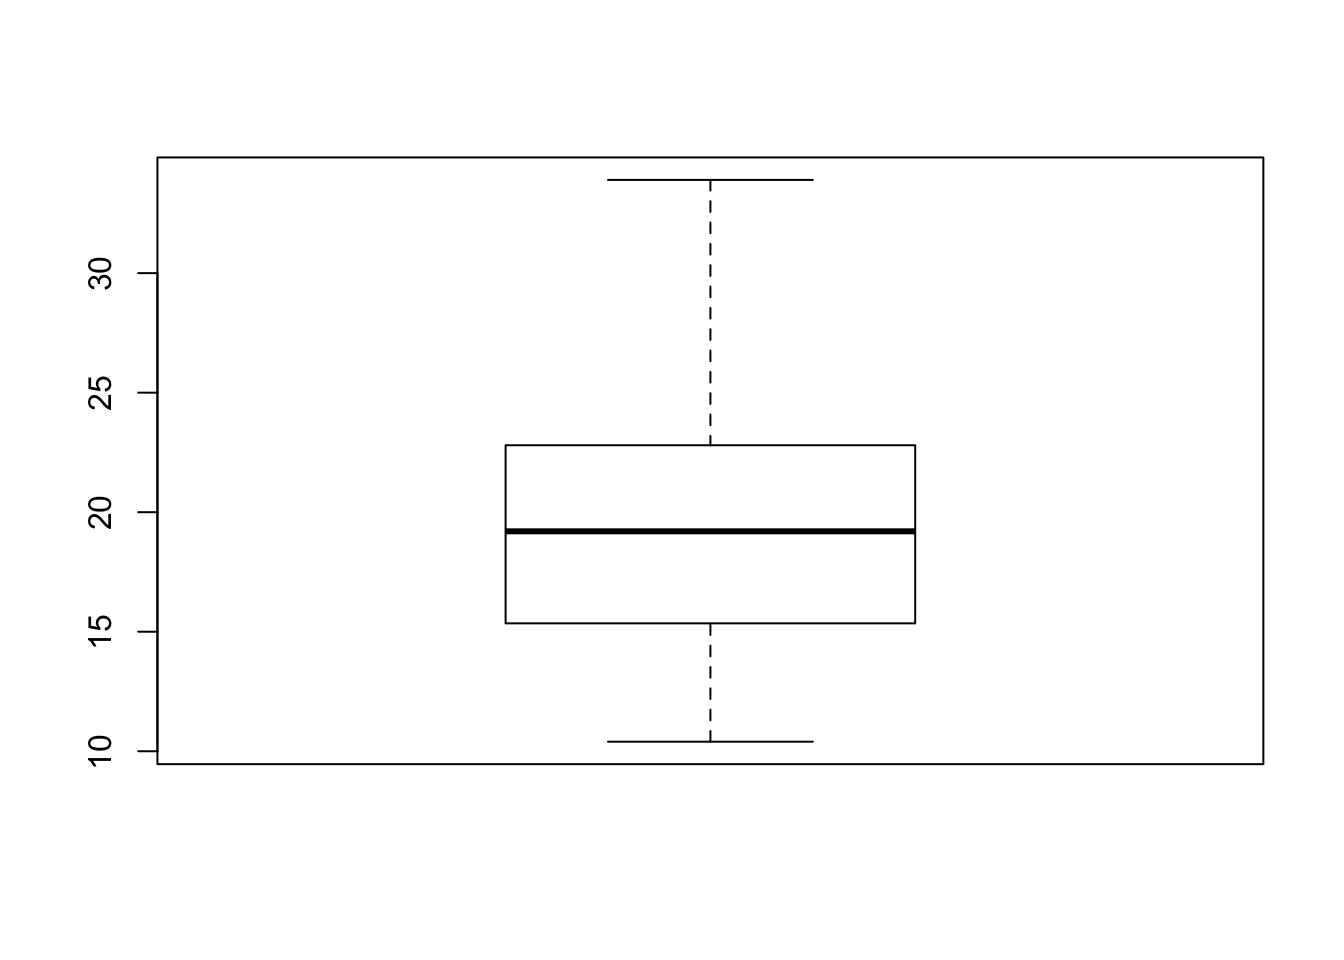
\includegraphics{Introduction-R_files/figure-latex/unnamed-chunk-51-1.pdf}

We recall that in a boxplot:

\begin{itemize}
\tightlist
\item
  The height (or length if we choose the option \texttt{horizontal\ =\ TRUE}) of the box is defined by the first and third quartiles \(q_1\) and \(q_3\).
\item
  The horizontal segment corresponds to the median \(m = q_2\).
\item
  The whisker at the bottom starts from \(q_1\) and goes down to the minimum of the sample if there are no extreme points on the left, ie values less than \(q_1-1.5\times (q_3-q_1)\). If there are extreme points on the left, the whisker stops precisely at the smallest point greater than the threshold \(q_1-1.5\times (q_3-q_1)\). In this case, we place the extreme points below the whisker.
\item
  Similarly, the whisker at the top starts from \(q_3\) and goes up to the maximum of the sample if there are no extreme points on the right, ie values greater than \(q_3+1.5 \times(q_3-q_1)\). If there are extreme points on the right, the whisker stops at the greatest point less than the threshold \(q_3+1.5\times (q_3-q_1)\), and we place the extreme points above of it.
\end{itemize}

Try the following:

\begin{Shaded}
\begin{Highlighting}[]
\NormalTok{u <-}\StringTok{ }\KeywordTok{c}\NormalTok{(mpg, }\FloatTok{3.5}\NormalTok{, }\FloatTok{2.7}\NormalTok{) }\CommentTok{# adding two very low values}
\KeywordTok{boxplot}\NormalTok{(u)}
\NormalTok{q1 <-}\StringTok{ }\KeywordTok{quantile}\NormalTok{(u, }\FloatTok{.25}\NormalTok{); q3 <-}\StringTok{ }\KeywordTok{quantile}\NormalTok{(u, }\FloatTok{.75}\NormalTok{)}
\KeywordTok{abline}\NormalTok{(}\DataTypeTok{h =} \KeywordTok{median}\NormalTok{(u), }\DataTypeTok{col =} \DecValTok{2}\NormalTok{, }\DataTypeTok{lwd =} \DecValTok{2}\NormalTok{)}
\KeywordTok{abline}\NormalTok{(}\DataTypeTok{h =}\NormalTok{ q1, }\DataTypeTok{col =} \DecValTok{2}\NormalTok{, }\DataTypeTok{lwd =} \DecValTok{2}\NormalTok{); }\KeywordTok{abline}\NormalTok{(}\DataTypeTok{h =}\NormalTok{ q3, }\DataTypeTok{col =} \DecValTok{2}\NormalTok{, }\DataTypeTok{lwd =} \DecValTok{2}\NormalTok{)}
\KeywordTok{abline}\NormalTok{(}\DataTypeTok{h =} \KeywordTok{max}\NormalTok{(u), }\DataTypeTok{col =} \DecValTok{3}\NormalTok{, }\DataTypeTok{lwd =} \DecValTok{2}\NormalTok{)}
\CommentTok{# u[u < q1-1.5*(q3-q1)] # extreme points on the left}
\KeywordTok{abline}\NormalTok{(}\DataTypeTok{h =} \KeywordTok{min}\NormalTok{(u[u }\OperatorTok{>=}\StringTok{ }\NormalTok{q1}\FloatTok{-1.5}\OperatorTok{*}\NormalTok{(q3}\OperatorTok{-}\NormalTok{q1)]), }\DataTypeTok{col =} \DecValTok{3}\NormalTok{, }\DataTypeTok{lwd =} \DecValTok{2}\NormalTok{)}
\KeywordTok{abline}\NormalTok{(}\DataTypeTok{h =} \KeywordTok{min}\NormalTok{(u), }\DataTypeTok{col =} \DecValTok{4}\NormalTok{, }\DataTypeTok{lwd =} \DecValTok{2}\NormalTok{)}
\end{Highlighting}
\end{Shaded}

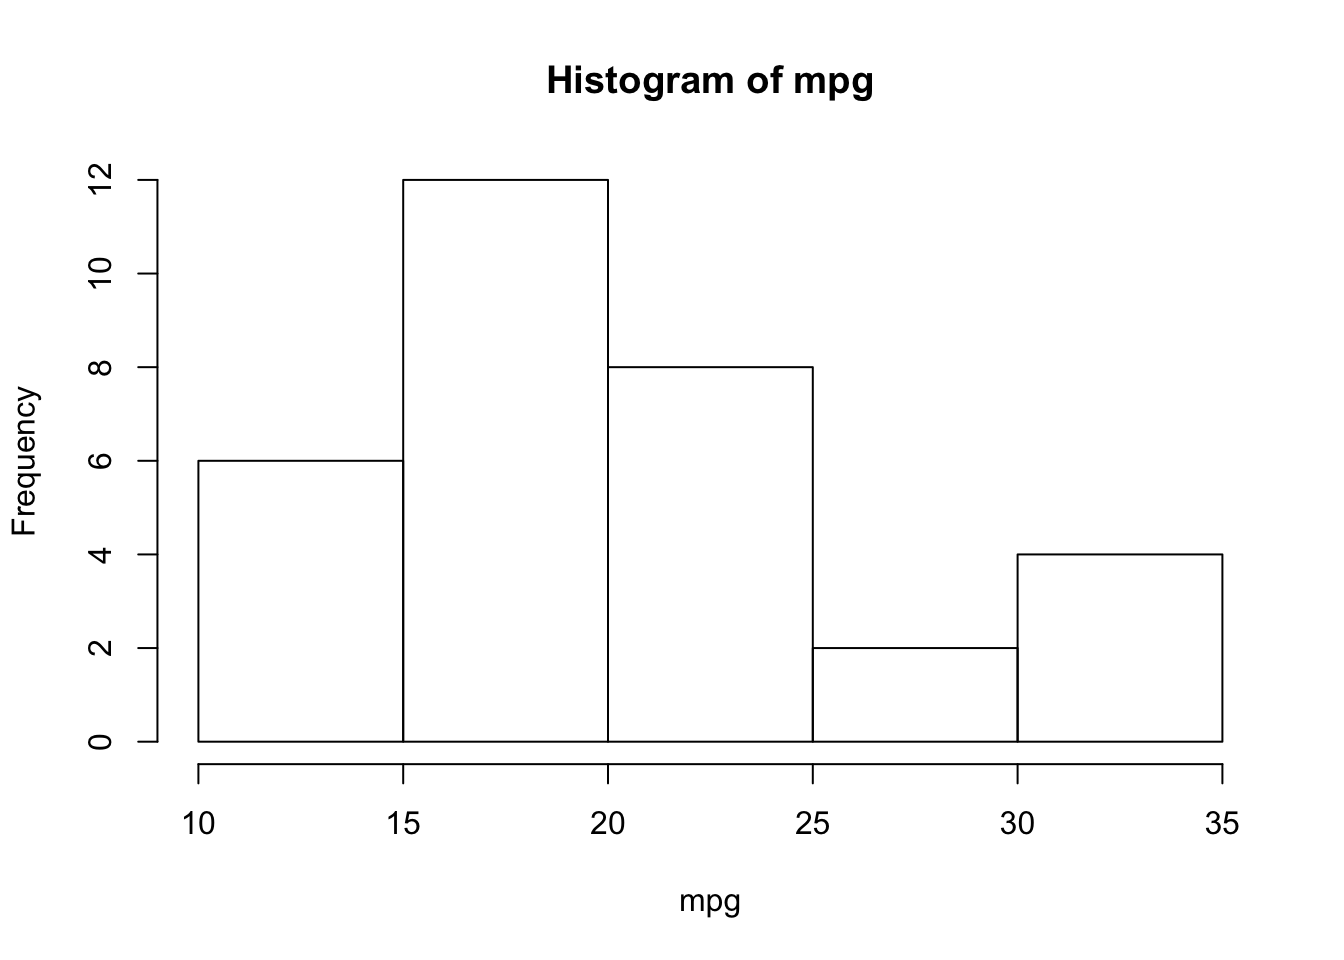
\includegraphics{Introduction-R_files/figure-latex/unnamed-chunk-52-1.pdf}

The other graphical tool to represent the distribution of a quantitative variable is the histogram:

\begin{Shaded}
\begin{Highlighting}[]
\KeywordTok{hist}\NormalTok{(mpg)}
\end{Highlighting}
\end{Shaded}

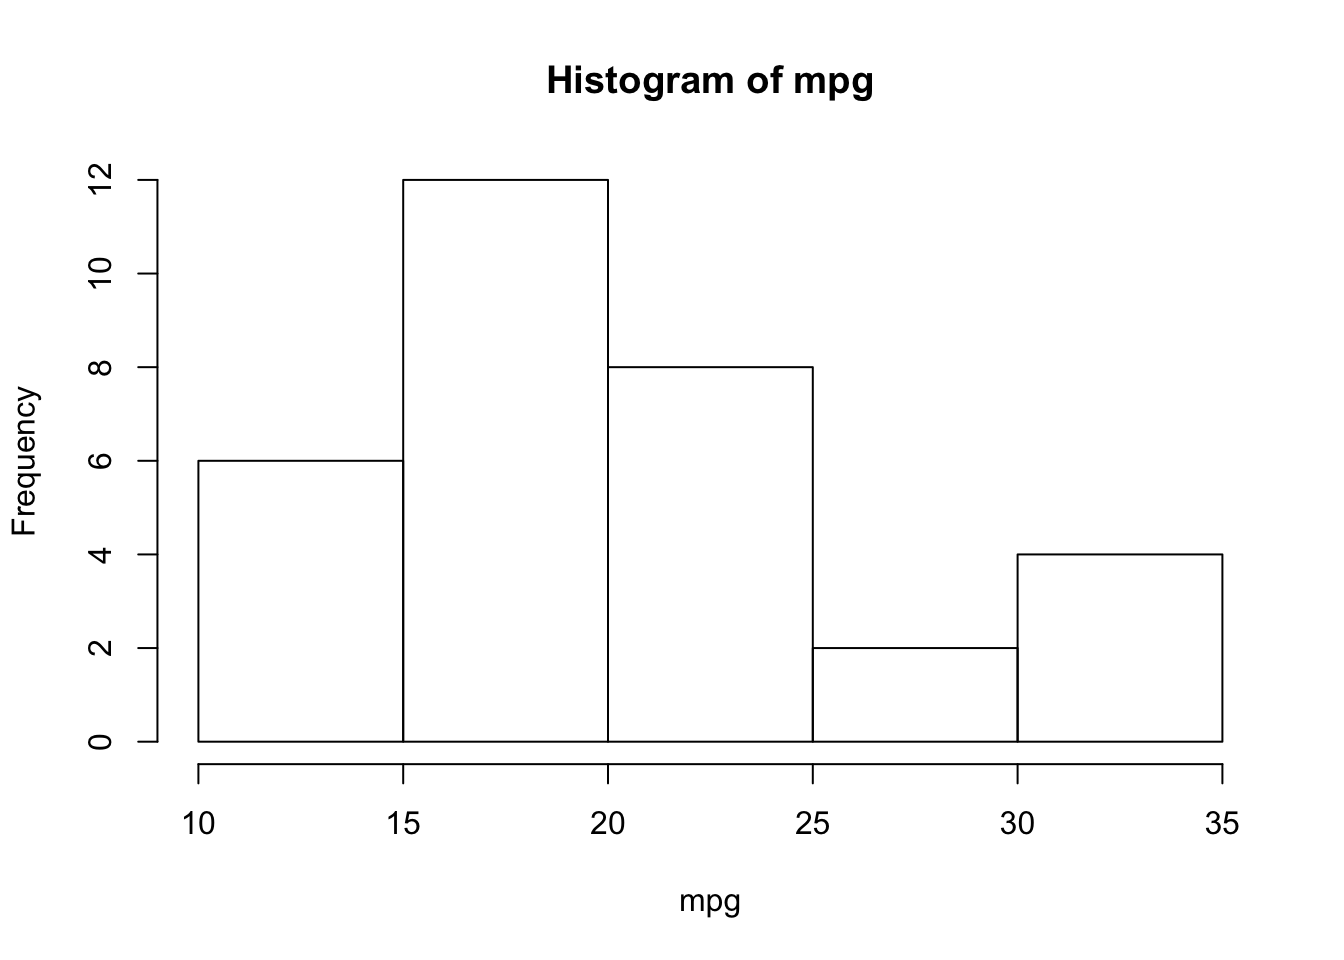
\includegraphics{Introduction-R_files/figure-latex/unnamed-chunk-53-1.pdf}

\begin{Shaded}
\begin{Highlighting}[]
\CommentTok{# Try the following:}
\CommentTok{# hist (mtcars$mpg, breaks = 20) # if we want 20 + 1 intervals}
\CommentTok{# we specify by hand the points which define the intervals:}
\CommentTok{# hist (mtcars$mpg, breaks = c (10, 15, 18, 20, 22, 25, 35))}
\end{Highlighting}
\end{Shaded}

By default the vertical axis gives the number of observations in each interval. If we want to plot the histogram in the \emph{density} scale, we have to use the option \texttt{freq\ =\ FALSE}. In this case we recall that the proportion of observations in each interval is given by the area of the corresponding rectangle:

\begin{Shaded}
\begin{Highlighting}[]
\KeywordTok{hist}\NormalTok{(mpg, }\DataTypeTok{freq =} \OtherTok{FALSE}\NormalTok{)}
\CommentTok{# relative frequency of observations in the [10,15] range:}
\CommentTok{# the area of the first rectangle is}
\CommentTok{# mean(10 <= mpg & mpg <= 15)}
\CommentTok{# to verify this, we divide the area by the base length and show}
\CommentTok{# that this is precisely the height of the rectangle:}
\KeywordTok{abline}\NormalTok{(}\DataTypeTok{h =} \KeywordTok{mean}\NormalTok{(}\DecValTok{10} \OperatorTok{<=}\StringTok{ }\NormalTok{mpg }\OperatorTok{&}\StringTok{ }\NormalTok{mpg }\OperatorTok{<=}\StringTok{ }\DecValTok{15}\NormalTok{)}\OperatorTok{/}\DecValTok{5}\NormalTok{, }\DataTypeTok{col =} \DecValTok{2}\NormalTok{)}
\end{Highlighting}
\end{Shaded}

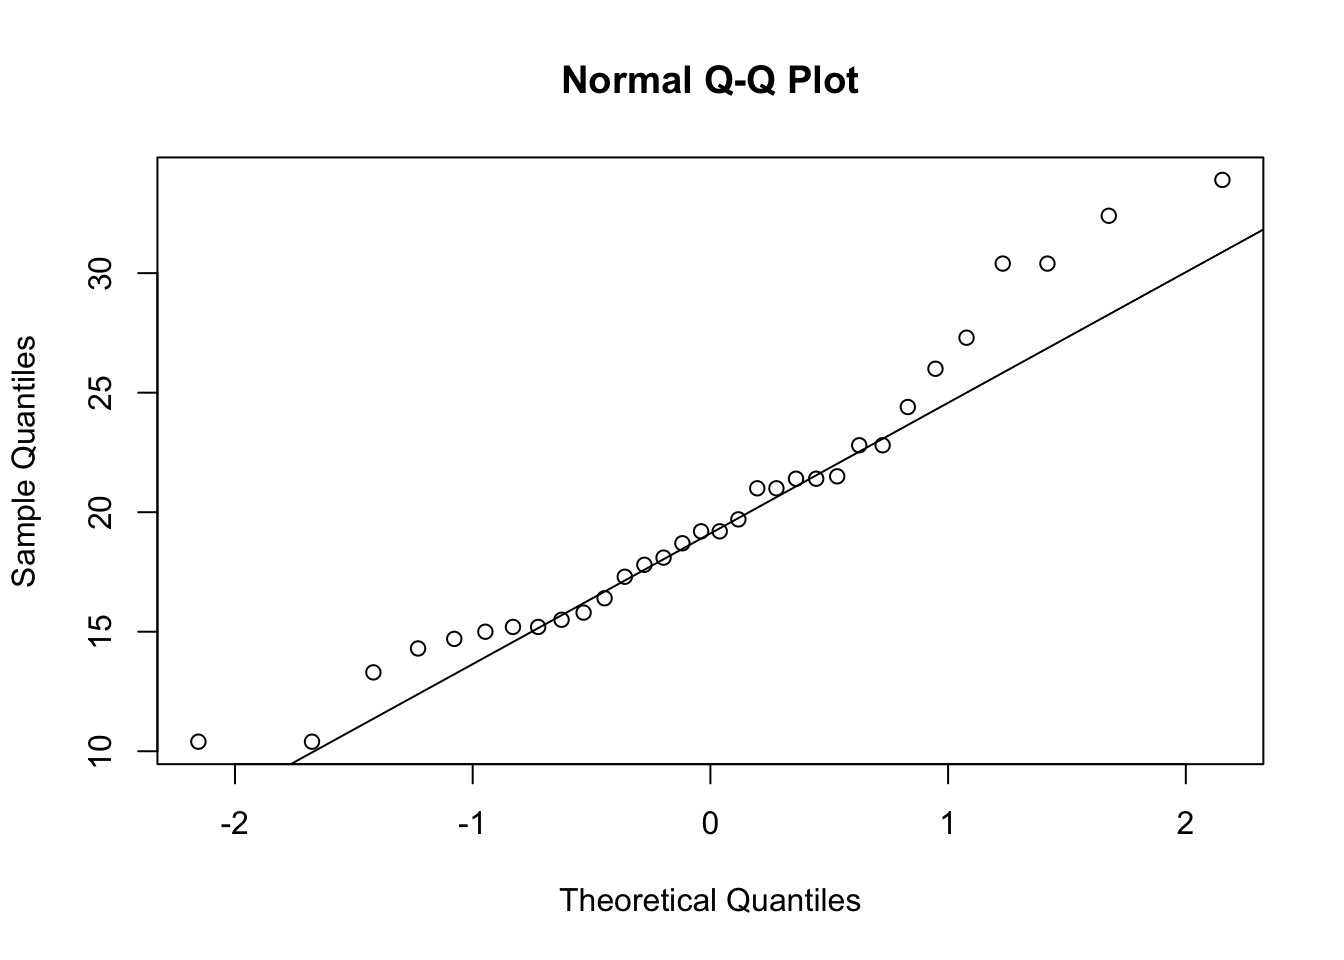
\includegraphics{Introduction-R_files/figure-latex/unnamed-chunk-54-1.pdf}

We can also compare the distribution of the sample with the theoretical distribution of the standard normal distribution through a \emph{QQ-plot}. This plot compare the empircal quantiles of the sample with the theoretical quantiles of the standard normal, if the observations in the sample were normally distributed than the points in the QQ-plot should be aligned along the bisector:

\begin{Shaded}
\begin{Highlighting}[]
\KeywordTok{qqnorm}\NormalTok{(mpg)}
\KeywordTok{qqline}\NormalTok{(mpg) }\CommentTok{# the line sample quantiles = theoretical quantiles}
\end{Highlighting}
\end{Shaded}

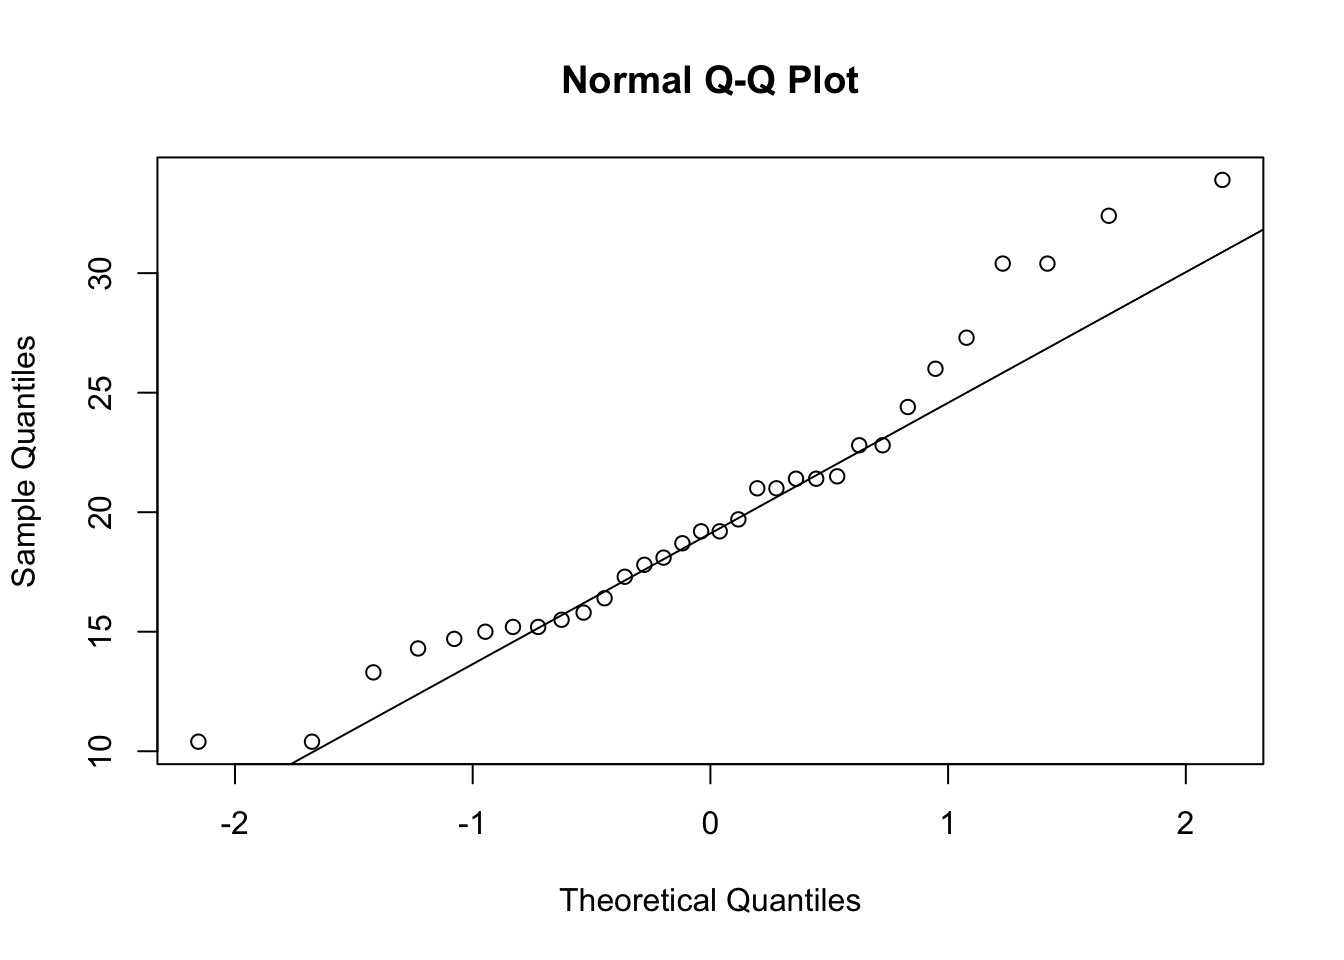
\includegraphics{Introduction-R_files/figure-latex/unnamed-chunk-55-1.pdf}

\textbf{Remark.} Compare the previous QQ-plot to that of the \emph{standardized} sample:

\begin{Shaded}
\begin{Highlighting}[]
\NormalTok{mpg.stand <-}\StringTok{ }\NormalTok{(mpg}\OperatorTok{-}\KeywordTok{mean}\NormalTok{(mpg))}\OperatorTok{/}\KeywordTok{sd}\NormalTok{(mpg) }\CommentTok{# we standardize mpg}
\KeywordTok{qqnorm}\NormalTok{(mpg.stand); }\KeywordTok{qqline}\NormalTok{(mpg.stand)}
\end{Highlighting}
\end{Shaded}

What happened? Note that the distribution of quantiles did not change:

\begin{Shaded}
\begin{Highlighting}[]
\KeywordTok{hist}\NormalTok{(}\KeywordTok{quantile}\NormalTok{(mpg))}
\KeywordTok{hist}\NormalTok{(}\KeywordTok{quantile}\NormalTok{(mpg.stand))}
\end{Highlighting}
\end{Shaded}

\hypertarget{qualitative-variables}{%
\subsection{Qualitative variables}\label{qualitative-variables}}

The \texttt{summary()} and \texttt{table()} functions applied to a factor (or a vector of characters) count the occurrences of the different levels.

\begin{Shaded}
\begin{Highlighting}[]
\KeywordTok{summary}\NormalTok{(cyl.factor)}
\end{Highlighting}
\end{Shaded}

\begin{verbatim}
##  4  6  8 
## 11  7 14
\end{verbatim}

\begin{Shaded}
\begin{Highlighting}[]
\KeywordTok{table}\NormalTok{(cyl.factor)}
\end{Highlighting}
\end{Shaded}

\begin{verbatim}
## cyl.factor
##  4  6  8 
## 11  7 14
\end{verbatim}

To get the proportions:

\begin{Shaded}
\begin{Highlighting}[]
\KeywordTok{prop.table}\NormalTok{(}\KeywordTok{table}\NormalTok{ (cyl.factor))}
\end{Highlighting}
\end{Shaded}

\begin{verbatim}
## cyl.factor
##       4       6       8 
## 0.34375 0.21875 0.43750
\end{verbatim}

If there are missing values, \texttt{summary\ ()} also counts the \texttt{NA}:

\begin{Shaded}
\begin{Highlighting}[]
\NormalTok{x <-}\StringTok{ }\KeywordTok{as.factor}\NormalTok{(}\KeywordTok{c}\NormalTok{(}\StringTok{'a'}\NormalTok{, }\StringTok{'a'}\NormalTok{, }\StringTok{'b'}\NormalTok{, }\StringTok{'c'}\NormalTok{, }\OtherTok{NA}\NormalTok{, }\StringTok{'c'}\NormalTok{))}
\KeywordTok{summary}\NormalTok{(x)}
\end{Highlighting}
\end{Shaded}

\begin{verbatim}
##    a    b    c NA's 
##    2    1    2    1
\end{verbatim}

\begin{Shaded}
\begin{Highlighting}[]
\KeywordTok{table}\NormalTok{(x)}
\end{Highlighting}
\end{Shaded}

\begin{verbatim}
## x
## a b c 
## 2 1 2
\end{verbatim}

\begin{Shaded}
\begin{Highlighting}[]
\KeywordTok{prop.table}\NormalTok{(}\KeywordTok{table}\NormalTok{(x)) }\CommentTok{# counts are divided by the total number of non-missing values}
\end{Highlighting}
\end{Shaded}

\begin{verbatim}
## x
##   a   b   c 
## 0.4 0.2 0.4
\end{verbatim}

\begin{Shaded}
\begin{Highlighting}[]
\KeywordTok{prop.table}\NormalTok{(}\KeywordTok{summary}\NormalTok{(x)) }\CommentTok{# counts are divided by the total number of values}
\end{Highlighting}
\end{Shaded}

\begin{verbatim}
##         a         b         c      NA's 
## 0.3333333 0.1666667 0.3333333 0.1666667
\end{verbatim}

We can use a \emph{bar plot} or a pie chart (not recommended) to represent occurrences:

\begin{Shaded}
\begin{Highlighting}[]
\KeywordTok{barplot}\NormalTok{(}\KeywordTok{table}\NormalTok{(cyl.factor))}
\end{Highlighting}
\end{Shaded}

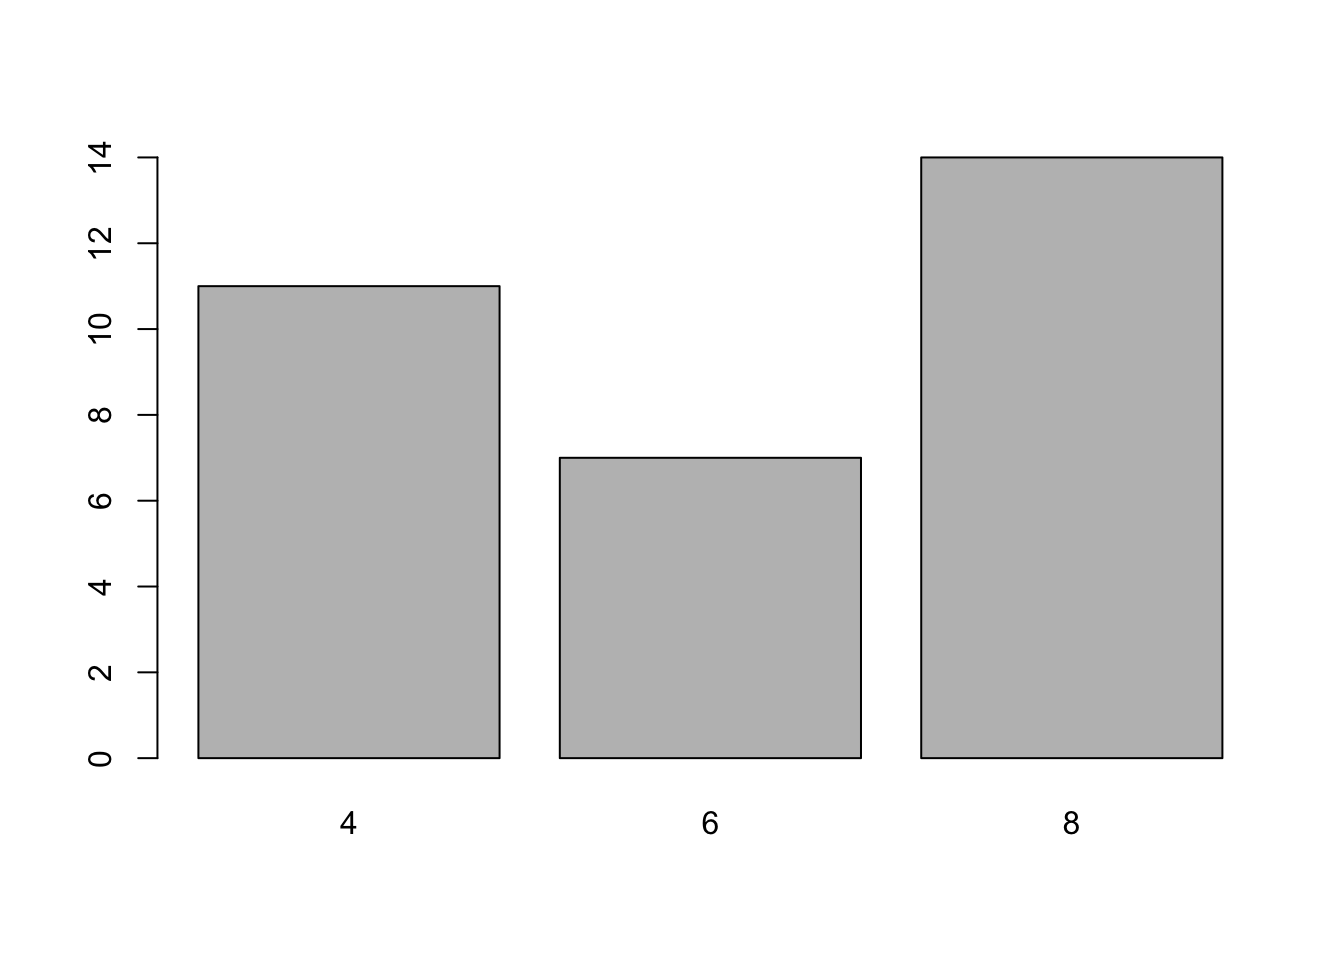
\includegraphics{Introduction-R_files/figure-latex/unnamed-chunk-61-1.pdf}

\begin{Shaded}
\begin{Highlighting}[]
\KeywordTok{pie}\NormalTok{(}\KeywordTok{summary}\NormalTok{(cyl.factor))}
\end{Highlighting}
\end{Shaded}

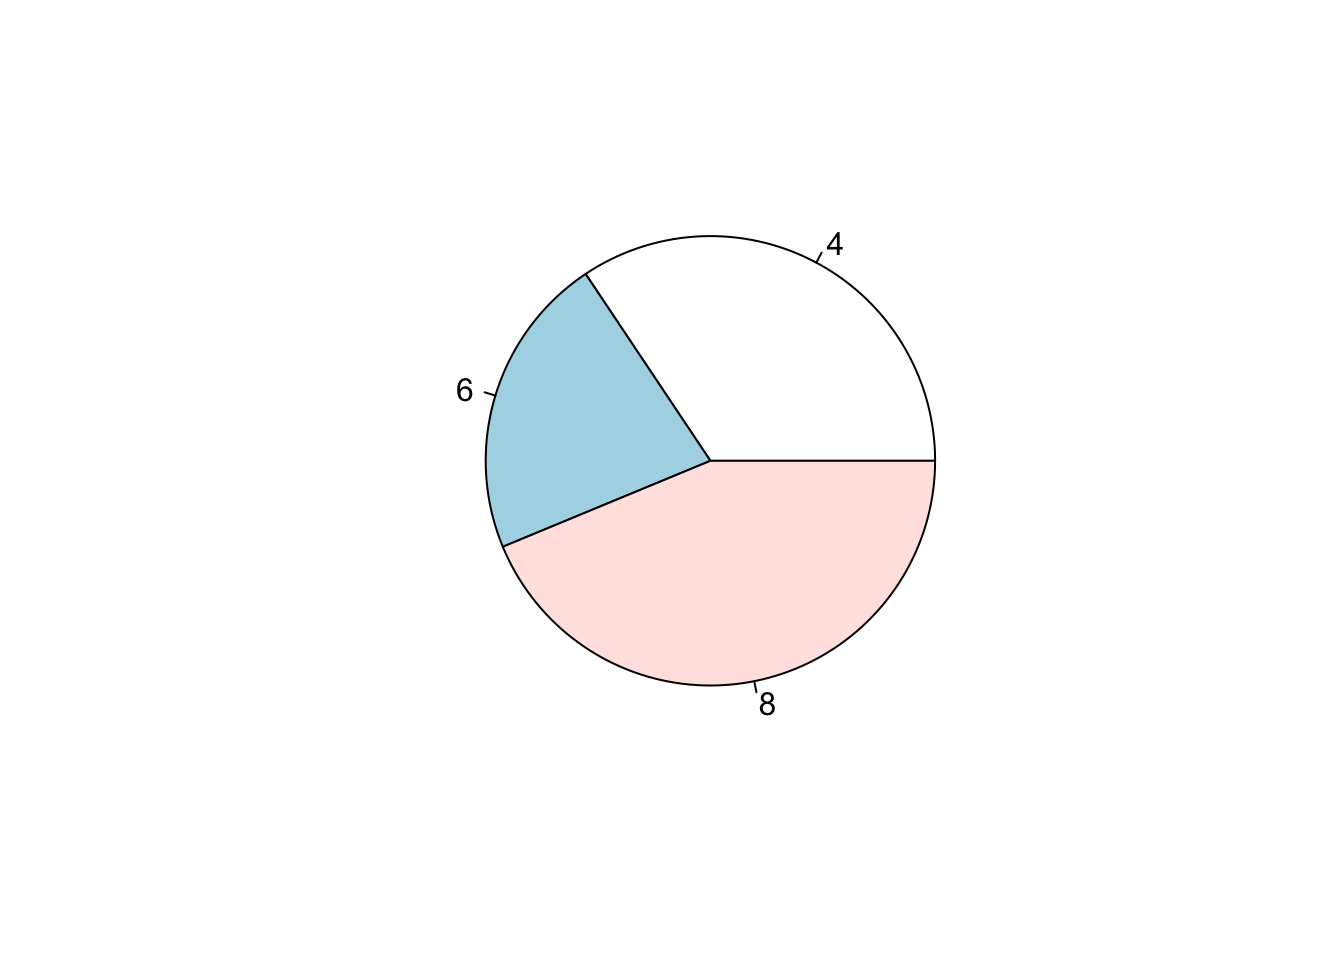
\includegraphics{Introduction-R_files/figure-latex/unnamed-chunk-61-2.pdf}

\hypertarget{bivariate-analysis}{%
\section{Bivariate analysis}\label{bivariate-analysis}}

\hypertarget{quantitative-variable-vs-quantitative-variable}{%
\subsection{Quantitative variable vs quantitative variable}\label{quantitative-variable-vs-quantitative-variable}}

We consider two quantitative variables measured on the same individuals.

For two quantitative variables, we can compute their covariance and linear correlation:

\begin{itemize}
\tightlist
\item
  the covariance measures the average joint deviation from the means of the two variables
\item
  Pearson's linear correlation coefficient \(\rho\) measures the intensity of linear dependence. \(\rho\) is comprised between \(-1\) and \(1\): its value is close to \(1\) (resp. \(-1\)) if there is a positive (resp. negative) linear dependence while its value is close to \(0\) if there is no linear dependence.
\end{itemize}

\begin{Shaded}
\begin{Highlighting}[]
\KeywordTok{cov}\NormalTok{(mpg, wt)}
\KeywordTok{cor}\NormalTok{(mpg, wt)}
\CommentTok{# Try this:}
\CommentTok{# cov(mpg, wt)/sd(mpg)/sd(wt)}
\end{Highlighting}
\end{Shaded}

Another type of correlation is Spearman's correlation measuring the linear correlation between the \emph{ranks} of the values of the two variables:

\begin{Shaded}
\begin{Highlighting}[]
\KeywordTok{cor}\NormalTok{(mpg, wt, }\DataTypeTok{method =} \StringTok{'spearman'}\NormalTok{)}
\CommentTok{# Try this}
\CommentTok{# cor(rank(mpg), rank(wt))}
\end{Highlighting}
\end{Shaded}

To graphically represent two quantitative variables we will use a a \emph{scatter plot:}

\begin{Shaded}
\begin{Highlighting}[]
\KeywordTok{plot}\NormalTok{(}\DataTypeTok{x =}\NormalTok{ wt, }\DataTypeTok{y =}\NormalTok{ mpg) }\CommentTok{# x, y = coordinates of the points}
\end{Highlighting}
\end{Shaded}

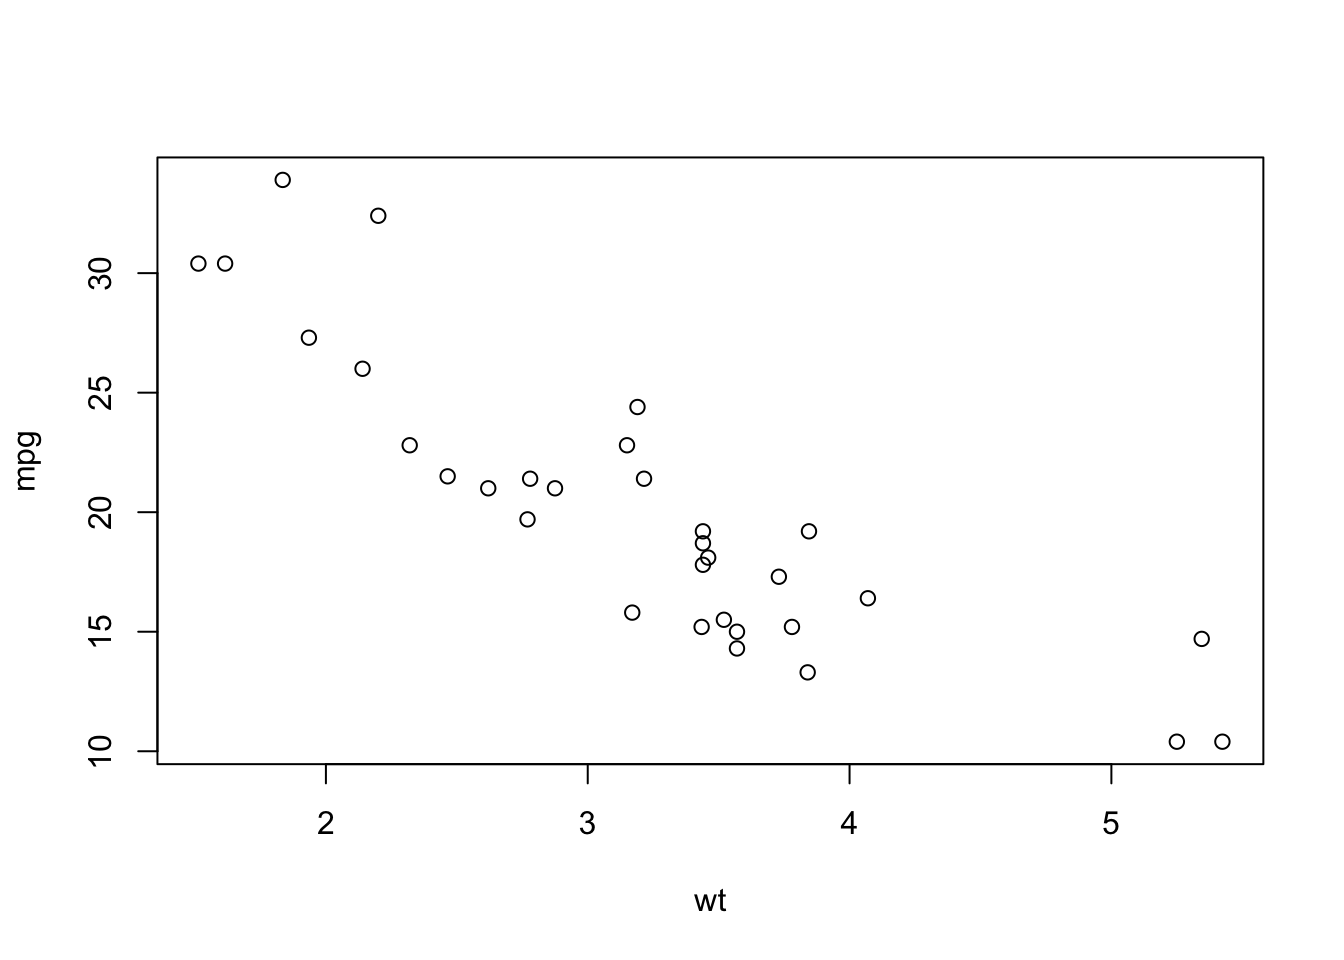
\includegraphics{Introduction-R_files/figure-latex/unnamed-chunk-64-1.pdf}

\begin{Shaded}
\begin{Highlighting}[]
\CommentTok{# Alternative: }
\CommentTok{# plot (wt ~ mpg) # where the ~ reads "wt according to mpg"}
\end{Highlighting}
\end{Shaded}

To find the least squares line (ie the linear model that best fits the data) and add it to the data:

\begin{Shaded}
\begin{Highlighting}[]
\NormalTok{m <-}\StringTok{ }\KeywordTok{lm}\NormalTok{(mpg }\OperatorTok{~}\StringTok{ }\NormalTok{wt)}
\KeywordTok{summary}\NormalTok{(m)}
\end{Highlighting}
\end{Shaded}

\begin{verbatim}
## 
## Call:
## lm(formula = mpg ~ wt)
## 
## Residuals:
##     Min      1Q  Median      3Q     Max 
## -4.5432 -2.3647 -0.1252  1.4096  6.8727 
## 
## Coefficients:
##             Estimate Std. Error t value Pr(>|t|)    
## (Intercept)  37.2851     1.8776  19.858  < 2e-16 ***
## wt           -5.3445     0.5591  -9.559 1.29e-10 ***
## ---
## Signif. codes:  0 '***' 0.001 '**' 0.01 '*' 0.05 '.' 0.1 ' ' 1
## 
## Residual standard error: 3.046 on 30 degrees of freedom
## Multiple R-squared:  0.7528,	Adjusted R-squared:  0.7446 
## F-statistic: 91.38 on 1 and 30 DF,  p-value: 1.294e-10
\end{verbatim}

\begin{Shaded}
\begin{Highlighting}[]
\CommentTok{# try:}
\CommentTok{# slope <- sum ((wt-mean(wt)) * (mpg-mean(mpg))) / sum((wt-mean (wt))^2)}
\CommentTok{# intercept <- mean (mpg) - slope * mean (wt)}
\KeywordTok{plot}\NormalTok{(mpg }\OperatorTok{~}\StringTok{ }\NormalTok{wt)}
\KeywordTok{abline}\NormalTok{(m, }\DataTypeTok{col =} \StringTok{"red"}\NormalTok{)}
\end{Highlighting}
\end{Shaded}

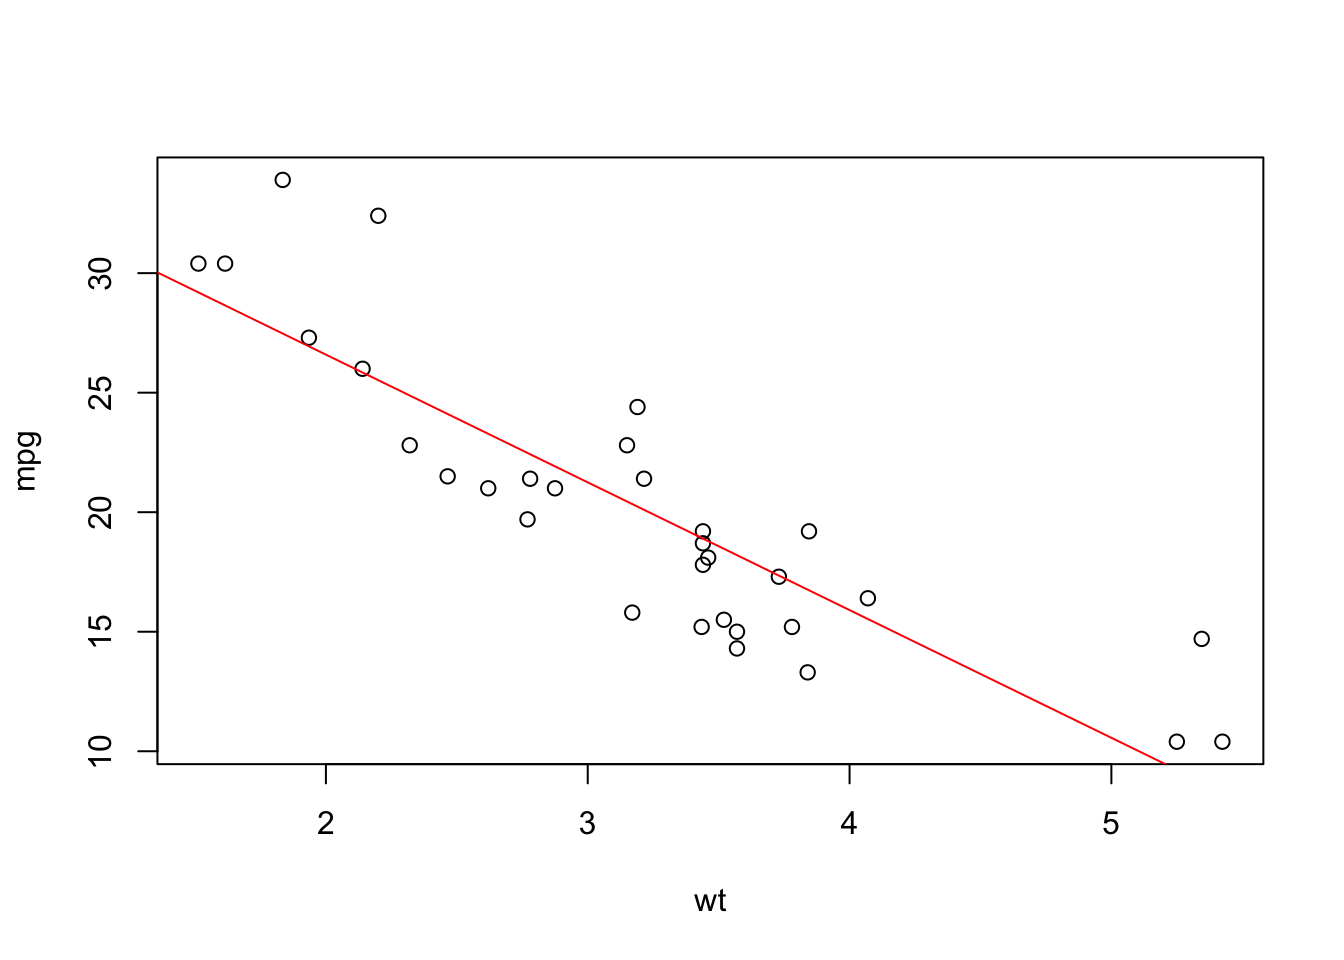
\includegraphics{Introduction-R_files/figure-latex/unnamed-chunk-65-1.pdf}

\hypertarget{qualitative-variable-vs-qualitative-variable}{%
\subsection{3.2 Qualitative variable vs qualitative variable}\label{qualitative-variable-vs-qualitative-variable}}

We consider two qualitative variables measured on the same individuals. For these variables, we can make contingency tables and calculate the total and marginal relative frequencies (in rows and columns). Try the following:

\begin{Shaded}
\begin{Highlighting}[]
\NormalTok{t <-}\StringTok{ }\KeywordTok{table}\NormalTok{(cyl, am)}
\CommentTok{# cyl and am are digital vectors,}
\CommentTok{# but to build the contingency table}
\CommentTok{# table() counts their terms.}
\NormalTok{t}
\KeywordTok{prop.table}\NormalTok{(t) }\CommentTok{# Prob(cyl, am)}
\KeywordTok{prop.table}\NormalTok{(t, }\DataTypeTok{margin =} \DecValTok{1}\NormalTok{) }\CommentTok{# P(am | cyl = 4), P(am | cyl = 6), P(am | cyl = 8)}
\KeywordTok{prop.table}\NormalTok{(t, }\DataTypeTok{margin =} \DecValTok{2}\NormalTok{) }\CommentTok{# P(cyl | am = 0), P(cyl | am = 1)}
\end{Highlighting}
\end{Shaded}

The corresponding graphic is the \emph{mosaic plot}:

\begin{Shaded}
\begin{Highlighting}[]
\KeywordTok{par}\NormalTok{(}\DataTypeTok{mfrow =} \KeywordTok{c}\NormalTok{ (}\DecValTok{1}\NormalTok{,}\DecValTok{2}\NormalTok{)) }\CommentTok{# to put two charts side by side}
\KeywordTok{mosaicplot}\NormalTok{(}\KeywordTok{table}\NormalTok{(cyl, am)) }\CommentTok{# P(am | cyl = 4), P(am | cyl = 6), P(am | cyl = 8)}
\KeywordTok{mosaicplot}\NormalTok{(}\KeywordTok{table}\NormalTok{(am, cyl)) }\CommentTok{# P(cyl | am = 0), P(cyl | am = 1)}
\end{Highlighting}
\end{Shaded}

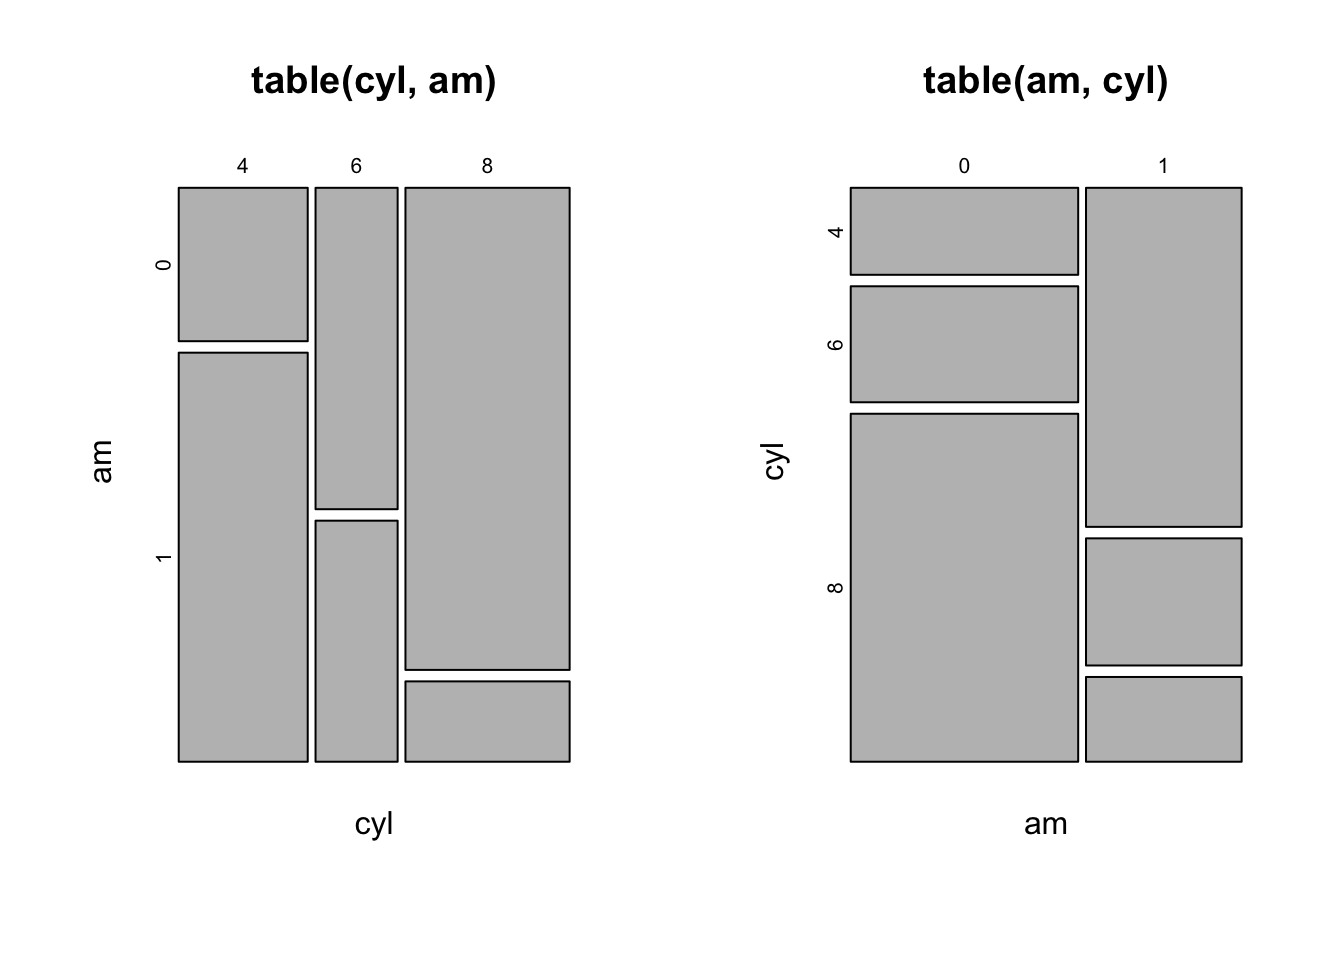
\includegraphics{Introduction-R_files/figure-latex/unnamed-chunk-67-1.pdf}

\hypertarget{quantitative-variable-vs-qualitative-variable}{%
\subsection{Quantitative variable vs qualitative variable}\label{quantitative-variable-vs-qualitative-variable}}

To evaluate a function \texttt{f} on the values of a \texttt{y} for each level of a factor \texttt{x} we use\texttt{tapply\ (X\ =\ y,\ INDEX\ =\ x,\ FUN\ =\ f)}. This is very useful when we want to calculate the statistics of a quantitative variable \texttt{y} grouped according to the levels of a qualitative variable\texttt{x}. To see this, try the following:

\begin{Shaded}
\begin{Highlighting}[]
\KeywordTok{tapply}\NormalTok{(mtcars}\OperatorTok{$}\NormalTok{mpg, mtcars}\OperatorTok{$}\NormalTok{cyl, mean) }\CommentTok{# the average miles per gallon according to the number of cylinders}
\KeywordTok{tapply}\NormalTok{(mtcars}\OperatorTok{$}\NormalTok{mpg, mtcars}\OperatorTok{$}\NormalTok{cyl, summary)}
\end{Highlighting}
\end{Shaded}

Graphically, we can build the boxplot of the quantitative variable for each level of qualitative variable:

\begin{Shaded}
\begin{Highlighting}[]
\KeywordTok{boxplot}\NormalTok{(mpg }\OperatorTok{~}\StringTok{ }\NormalTok{cyl, }\DataTypeTok{data =}\NormalTok{ mtcars)}
\end{Highlighting}
\end{Shaded}

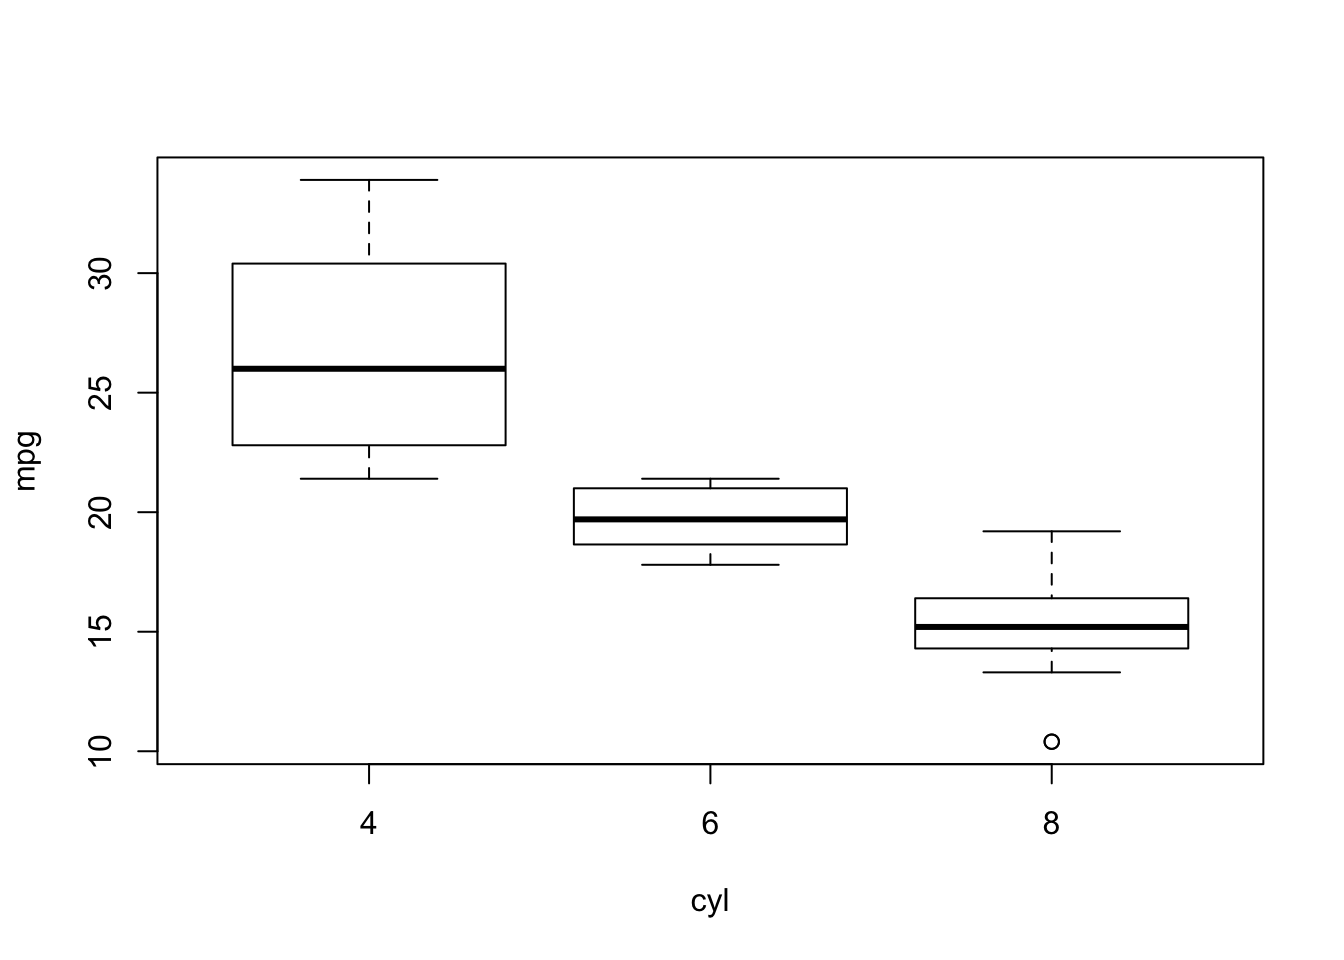
\includegraphics{Introduction-R_files/figure-latex/unnamed-chunk-69-1.pdf}

\hypertarget{base-graphics}{%
\chapter{Base graphics}\label{base-graphics}}

\hypertarget{basic-constructions-and-scatter-plots}{%
\section{Basic constructions and scatter plots}\label{basic-constructions-and-scatter-plots}}

We have already seen how to add a line to a scatter plot, to complete the graph we can specify a title, change the axis labels, and add a legend:

\begin{Shaded}
\begin{Highlighting}[]
\KeywordTok{plot}\NormalTok{(wt, mpg,}
     \DataTypeTok{main =} \StringTok{'Weight and consumption of cars'}\NormalTok{,}
     \DataTypeTok{xlab =} \StringTok{'weight'}\NormalTok{, }\DataTypeTok{ylab =} \StringTok{'consumption'}\NormalTok{) }\CommentTok{# xlab = label x axis}
\KeywordTok{abline}\NormalTok{(}\DataTypeTok{h =} \KeywordTok{mean}\NormalTok{ (mpg), }\DataTypeTok{col =} \DecValTok{2}\NormalTok{, }\DataTypeTok{lty =} \DecValTok{2}\NormalTok{) }\CommentTok{# h = horizontal line, col = color, lty = line type}
\KeywordTok{legend}\NormalTok{(}\DataTypeTok{x =} \StringTok{'topright'}\NormalTok{, }\DataTypeTok{lty =} \DecValTok{2}\NormalTok{, }\DataTypeTok{col =} \DecValTok{2}\NormalTok{, }\DataTypeTok{legend =} \StringTok{'average consumption'}\NormalTok{)}
\end{Highlighting}
\end{Shaded}

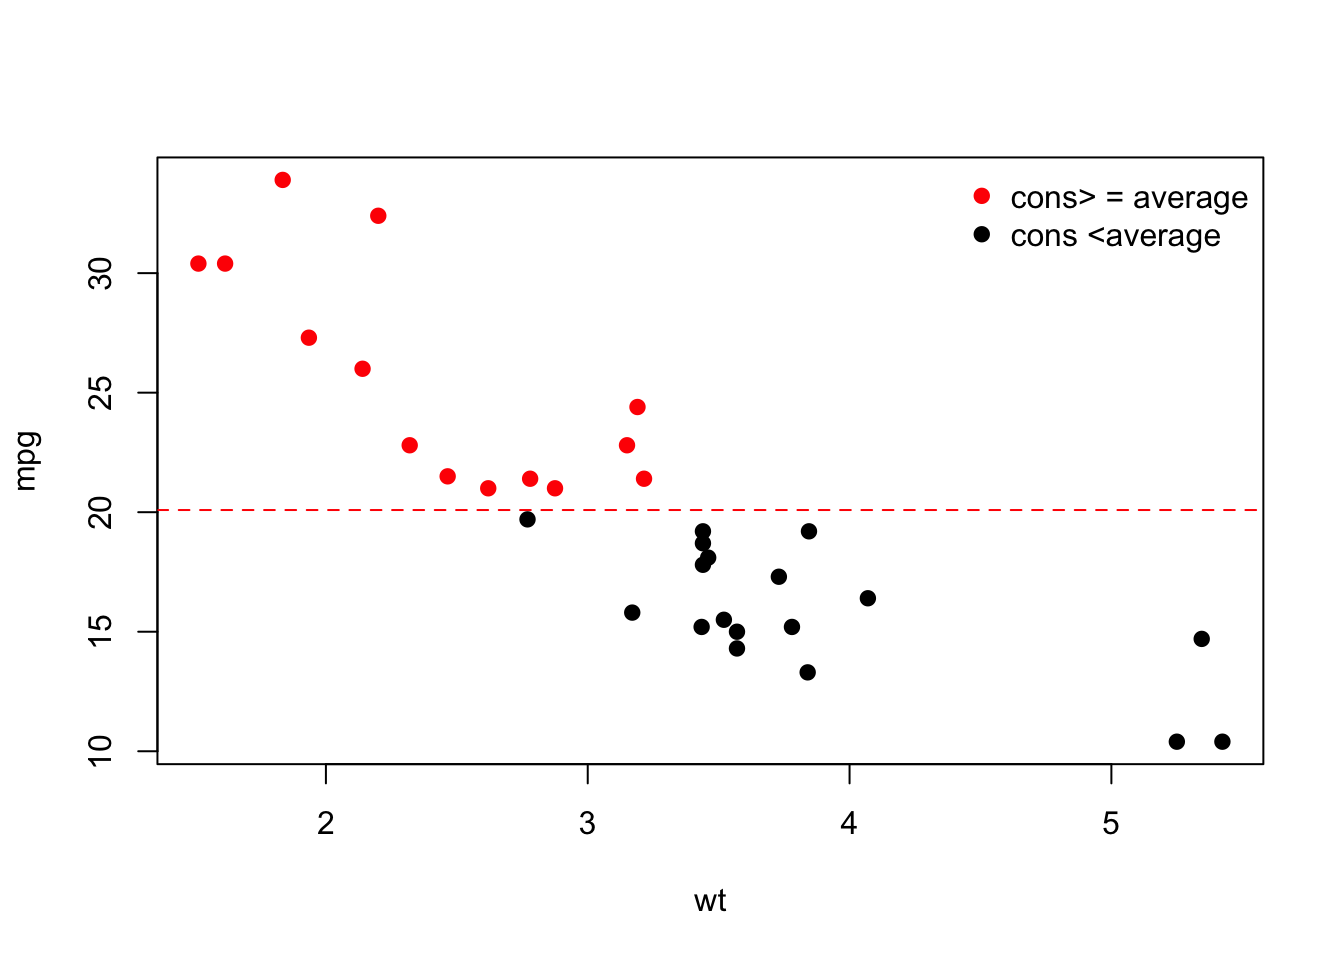
\includegraphics{Introduction-R_files/figure-latex/unnamed-chunk-70-1.pdf}

\begin{Shaded}
\begin{Highlighting}[]
\CommentTok{# x = legend location}
\end{Highlighting}
\end{Shaded}

We can also add a third dimension by coloring the points according to a condition:

\begin{Shaded}
\begin{Highlighting}[]
\KeywordTok{plot}\NormalTok{(wt, mpg,}
     \DataTypeTok{pch =} \DecValTok{19}\NormalTok{, }\CommentTok{# pch = type of point}
     \DataTypeTok{col =}\NormalTok{ (mpg }\OperatorTok{>=}\StringTok{ }\KeywordTok{mean}\NormalTok{ (mpg)) }\OperatorTok{+}\StringTok{ }\DecValTok{1} \CommentTok{# 1 = black, 2 = red}
\NormalTok{)}
\KeywordTok{abline}\NormalTok{(}\DataTypeTok{h =} \KeywordTok{mean}\NormalTok{(mpg), }\DataTypeTok{col =} \DecValTok{2}\NormalTok{, }\DataTypeTok{lty =} \DecValTok{2}\NormalTok{) }\CommentTok{# h = horizontal line, col = color, lty = line type}
\KeywordTok{legend}\NormalTok{(}\DataTypeTok{x =} \StringTok{'topright'}\NormalTok{,}
       \DataTypeTok{pch =} \DecValTok{19}\NormalTok{,}
       \DataTypeTok{col =} \DecValTok{2}\OperatorTok{:}\StringTok{ }\DecValTok{1}\NormalTok{,}
       \DataTypeTok{legend =} \KeywordTok{c}\NormalTok{ (}\StringTok{'cons> = average'}\NormalTok{, }\StringTok{'cons <average'}\NormalTok{), }\CommentTok{# legend = vector with labels}
       \DataTypeTok{bty =} \StringTok{'n'} \CommentTok{# no frame around the legend}
\NormalTok{)}
\end{Highlighting}
\end{Shaded}

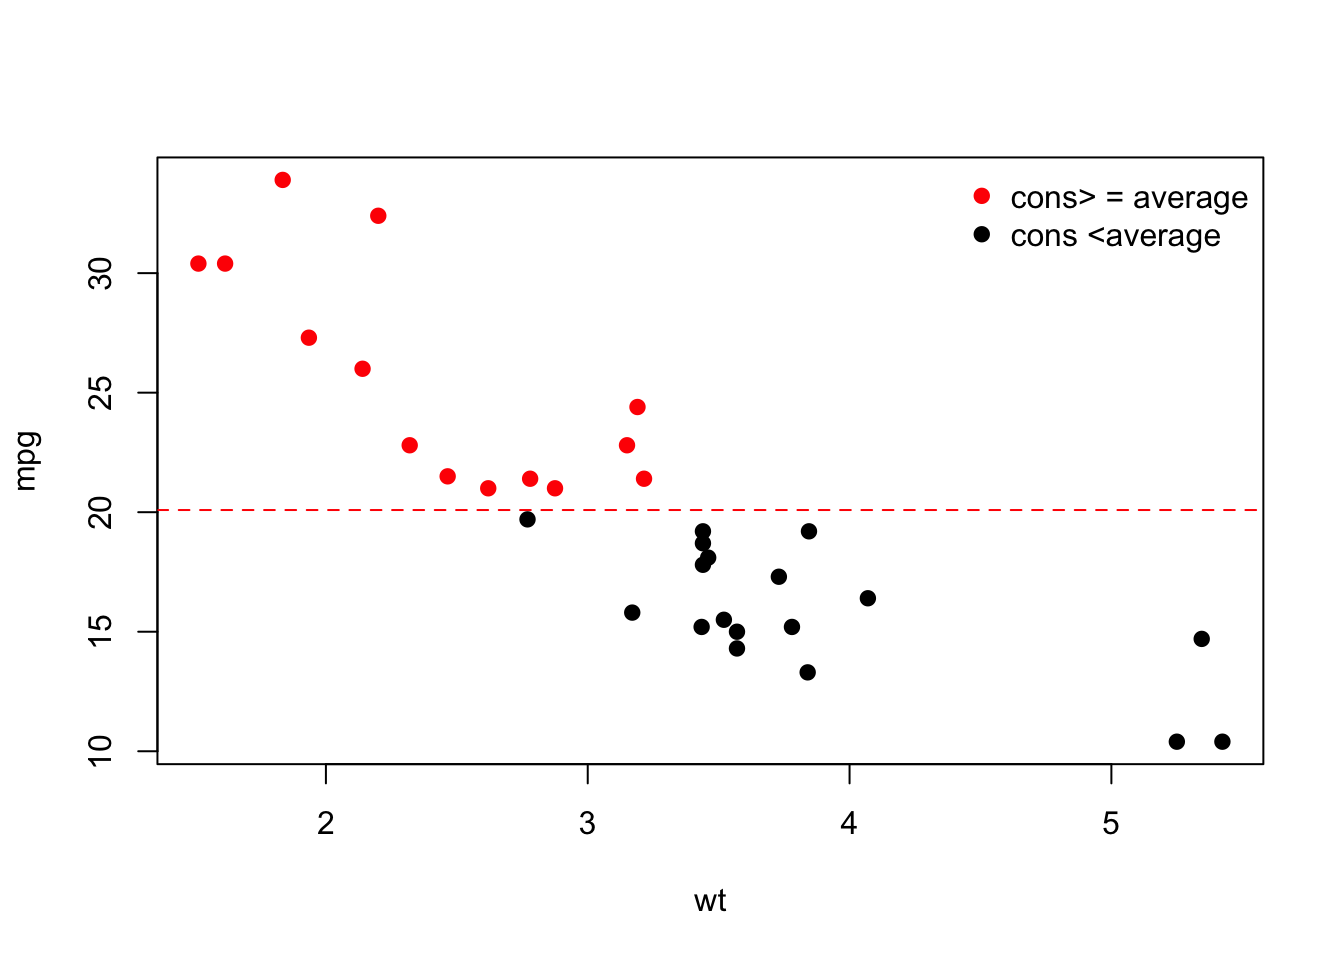
\includegraphics{Introduction-R_files/figure-latex/unnamed-chunk-71-1.pdf}

In general, \texttt{abline(a,\ b)} allows to add a line with intercept \texttt{a} and slope\texttt{b} to an existing plot. For example, an alternative way to add the regression line is as follows:

\begin{Shaded}
\begin{Highlighting}[]
\NormalTok{intercept =}\StringTok{ }\KeywordTok{coef}\NormalTok{(m)[}\DecValTok{1}\NormalTok{]}
\NormalTok{slope =}\StringTok{ }\KeywordTok{coef}\NormalTok{(m)[}\DecValTok{2}\NormalTok{]}
\KeywordTok{plot}\NormalTok{(wt, mpg, }\DataTypeTok{main =} \StringTok{'Line of least squares'}\NormalTok{)}
\KeywordTok{abline}\NormalTok{(}\DataTypeTok{a =}\NormalTok{ intercept, }\DataTypeTok{b =}\NormalTok{ slope)}
\end{Highlighting}
\end{Shaded}

To add any line (not necessarily a straight line) we use the \texttt{lines()} function. For example, to add the \emph{lowess} (locally-weighted polynomial regression) smoothing curve:

\begin{Shaded}
\begin{Highlighting}[]
\KeywordTok{plot}\NormalTok{(wt, mpg, }\DataTypeTok{main =} \StringTok{'Smoothing curve'}\NormalTok{)}
\KeywordTok{lines}\NormalTok{(}\KeywordTok{lowess}\NormalTok{ (mpg }\OperatorTok{~}\StringTok{ }\NormalTok{wt), }\CommentTok{# lines (): to add a curve}
      \DataTypeTok{col =} \StringTok{'blue'}\NormalTok{, }\CommentTok{# same as col = 4}
      \DataTypeTok{lwd =} \DecValTok{2}\NormalTok{) }\CommentTok{# lwd = line thickness}
\end{Highlighting}
\end{Shaded}

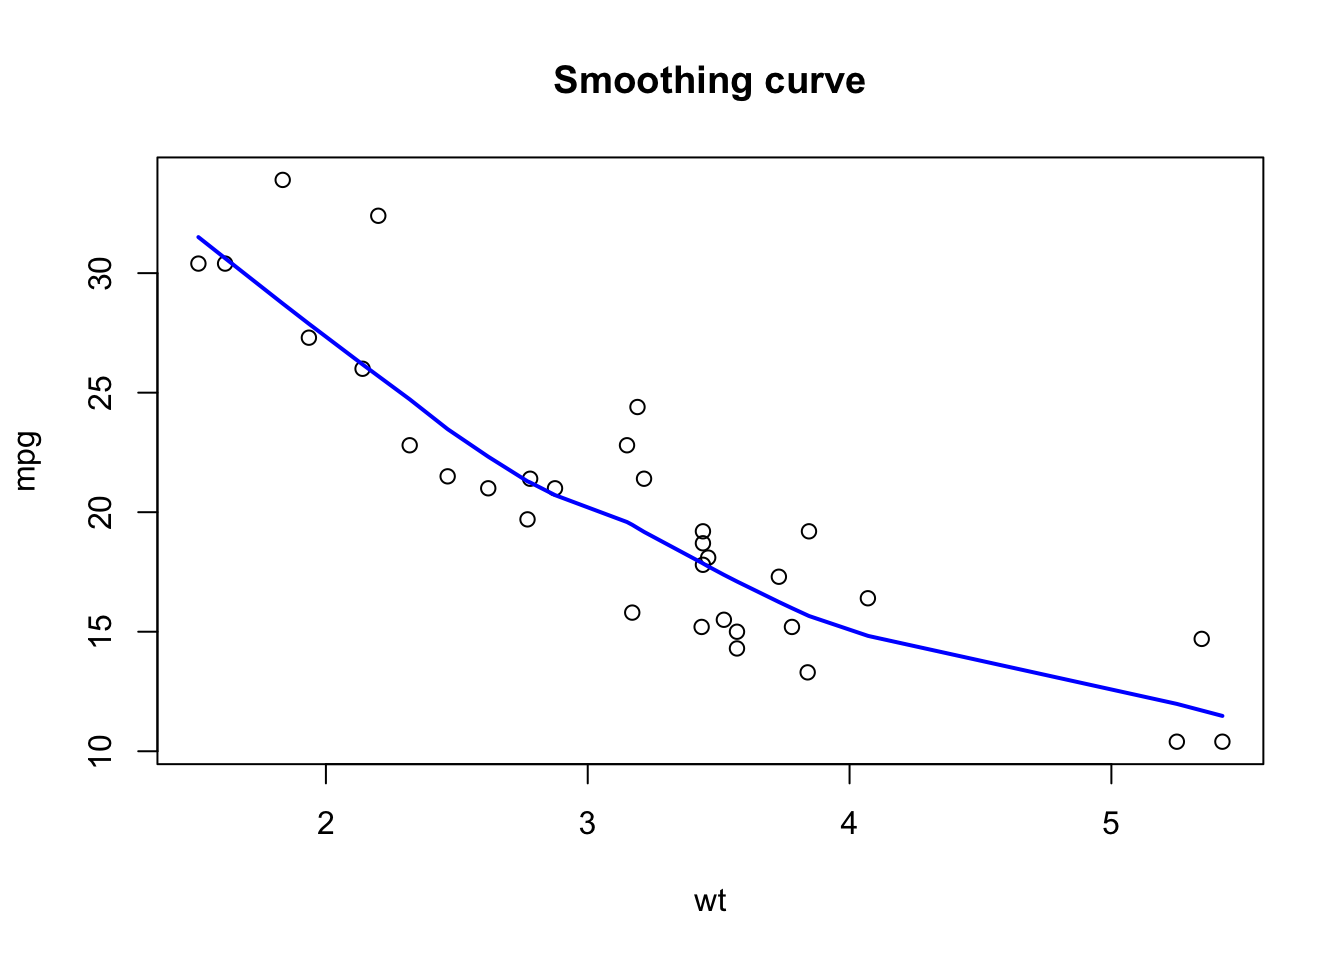
\includegraphics{Introduction-R_files/figure-latex/unnamed-chunk-73-1.pdf}

We can add new points using \texttt{points()}:

\begin{Shaded}
\begin{Highlighting}[]
\KeywordTok{plot}\NormalTok{(wt, mpg, }\DataTypeTok{main =} \StringTok{'Smoothing curves'}\NormalTok{)}
\KeywordTok{lines}\NormalTok{(}\KeywordTok{lowess}\NormalTok{ (mpg }\OperatorTok{~}\StringTok{ }\NormalTok{wt), }\DataTypeTok{col =} \StringTok{'blue'}\NormalTok{, }\DataTypeTok{lwd =} \DecValTok{2}\NormalTok{)}
\NormalTok{outliers =}\StringTok{ }\KeywordTok{cbind}\NormalTok{(}\KeywordTok{c}\NormalTok{(}\FloatTok{4.5}\NormalTok{,}\FloatTok{4.6}\NormalTok{,}\DecValTok{5}\NormalTok{), }\KeywordTok{c}\NormalTok{(}\DecValTok{26}\NormalTok{,}\DecValTok{26}\NormalTok{,}\DecValTok{30}\NormalTok{))}
\KeywordTok{points}\NormalTok{(outliers, }\DataTypeTok{pch =} \DecValTok{2}\NormalTok{) }\CommentTok{# pch = 2 for triangles}
\KeywordTok{lines}\NormalTok{(}\KeywordTok{lowess}\NormalTok{ (}\KeywordTok{c}\NormalTok{ (wt, outliers[, }\DecValTok{1}\NormalTok{]),}
              \KeywordTok{c}\NormalTok{ (mpg, outliers[, }\DecValTok{2}\NormalTok{])),}
      \DataTypeTok{col =} \DecValTok{2}\NormalTok{, }\DataTypeTok{lwd =} \DecValTok{2}\NormalTok{)}
\KeywordTok{legend}\NormalTok{ (}\DataTypeTok{x =} \StringTok{'bottomleft'}\NormalTok{, }\DataTypeTok{col =} \KeywordTok{c}\NormalTok{ (}\DecValTok{4}\NormalTok{,}\DecValTok{2}\NormalTok{), }\DataTypeTok{lwd =} \DecValTok{2}\NormalTok{, }\DataTypeTok{legend =} \KeywordTok{c}\NormalTok{ (}\StringTok{'without outliers'}\NormalTok{, }\StringTok{'with outliers'}\NormalTok{), }\DataTypeTok{bty =} \StringTok{'n'}\NormalTok{)}
\end{Highlighting}
\end{Shaded}

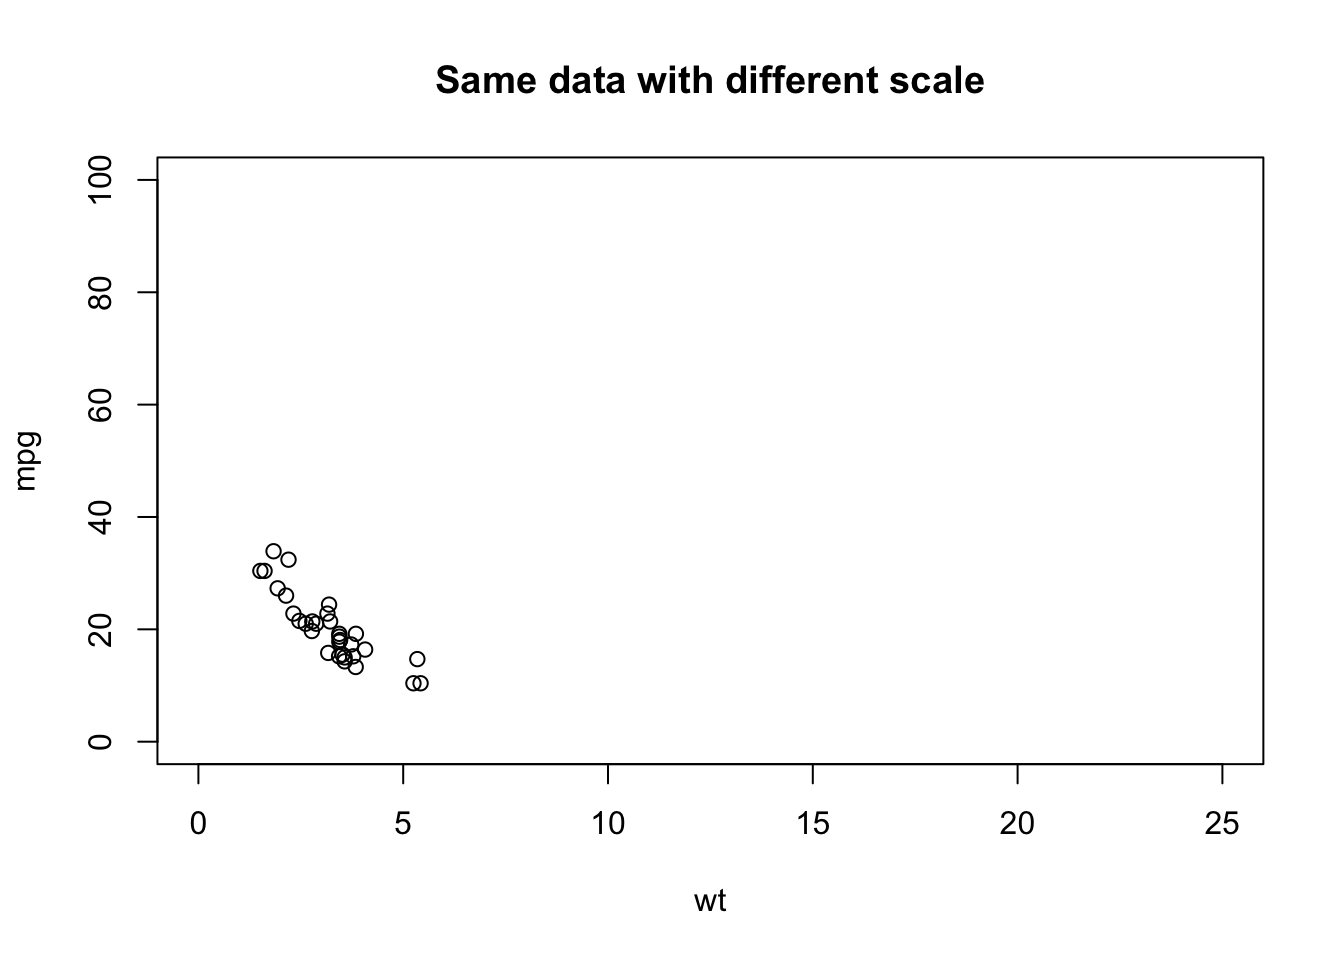
\includegraphics{Introduction-R_files/figure-latex/unnamed-chunk-74-1.pdf}

We can control the range of axes using \texttt{xlim()} and \texttt{ylim()}:

\begin{Shaded}
\begin{Highlighting}[]
\KeywordTok{plot}\NormalTok{(wt, mpg, }\DataTypeTok{main =} \StringTok{'Same data with different scale'}\NormalTok{,}
     \DataTypeTok{xlim =} \KeywordTok{c}\NormalTok{ (}\DecValTok{0}\NormalTok{, }\DecValTok{25}\NormalTok{),}
     \DataTypeTok{ylim =} \KeywordTok{c}\NormalTok{ (}\DecValTok{0}\NormalTok{, }\DecValTok{100}\NormalTok{))}
\end{Highlighting}
\end{Shaded}

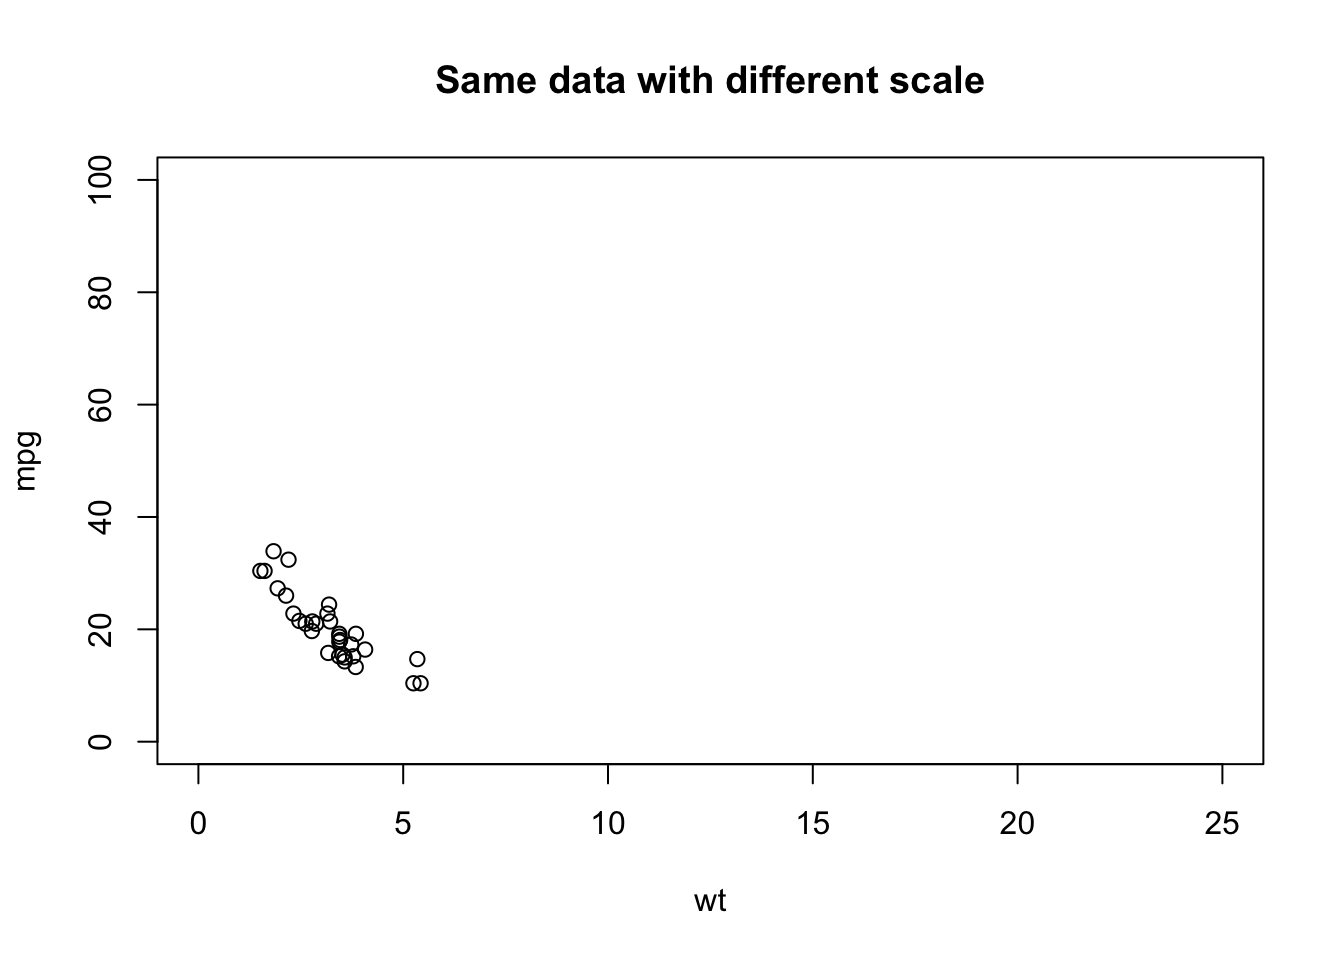
\includegraphics{Introduction-R_files/figure-latex/unnamed-chunk-75-1.pdf}

\hypertarget{line-graphs}{%
\section{Line graphs}\label{line-graphs}}

The \texttt{lines()} function adds a line to an existing graph and cannot be used to create a new graph. To draw a line connecting the successive elements of a vector we will rather use \texttt{plot(x\ =\ vector,\ type\ =\ l)}:

\begin{Shaded}
\begin{Highlighting}[]
\NormalTok{mydata =}\StringTok{ }\KeywordTok{cos}\NormalTok{(}\DecValTok{2} \OperatorTok{*}\StringTok{ }\NormalTok{pi }\OperatorTok{/}\StringTok{ }\DecValTok{12} \OperatorTok{*}\StringTok{ }\NormalTok{(}\DecValTok{1}\OperatorTok{:}\DecValTok{36}\NormalTok{)) }\OperatorTok{+}\StringTok{ }\KeywordTok{rnorm}\NormalTok{ (}\DecValTok{36}\NormalTok{,}\DecValTok{0}\NormalTok{, }\FloatTok{.2}\NormalTok{) }\CommentTok{# data simulation}
\KeywordTok{plot}\NormalTok{(mydata, }\DataTypeTok{type =} \StringTok{'l'}\NormalTok{, }\DataTypeTok{main =} \StringTok{'type = l'}\NormalTok{)}
\end{Highlighting}
\end{Shaded}

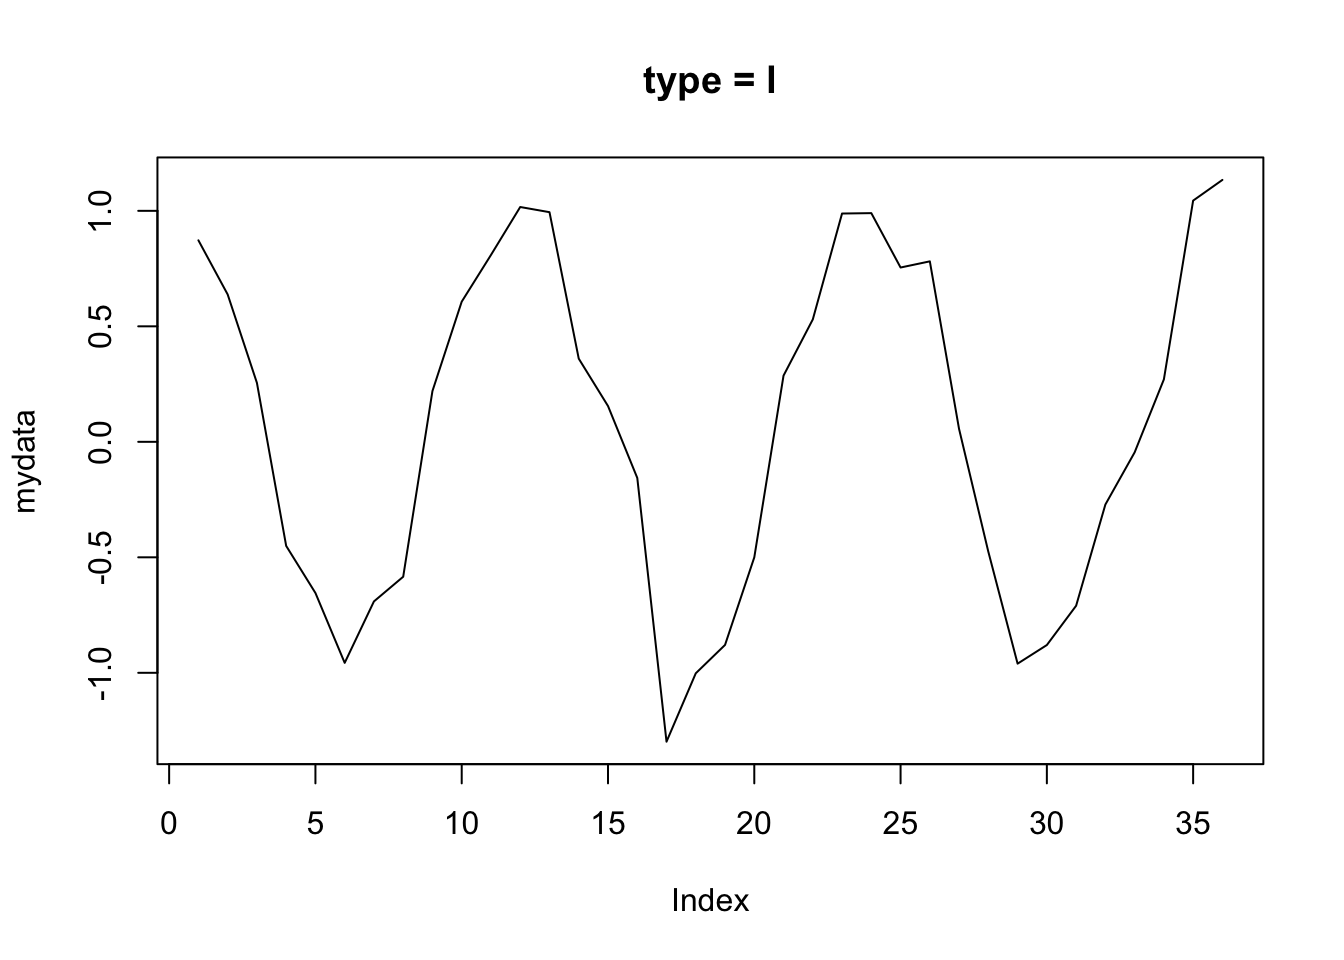
\includegraphics{Introduction-R_files/figure-latex/unnamed-chunk-76-1.pdf}

The \texttt{type} parameter allows you to connect (or not) the points in different ways:

\begin{Shaded}
\begin{Highlighting}[]
\KeywordTok{par}\NormalTok{(}\DataTypeTok{mfrow =} \KeywordTok{c}\NormalTok{ (}\DecValTok{2}\NormalTok{,}\DecValTok{2}\NormalTok{)) }\CommentTok{# explained in the next section}
\KeywordTok{plot}\NormalTok{(mydata, }\DataTypeTok{type =} \StringTok{'p'}\NormalTok{, }\DataTypeTok{main =} \StringTok{'type = p'}\NormalTok{) }\CommentTok{# default}
\KeywordTok{plot}\NormalTok{(mydata, }\DataTypeTok{type =} \StringTok{'o'}\NormalTok{, }\DataTypeTok{main =} \StringTok{'type = o'}\NormalTok{)}
\KeywordTok{plot}\NormalTok{(}\DecValTok{1}\OperatorTok{:}\StringTok{ }\DecValTok{10}\NormalTok{, }\DataTypeTok{type =} \StringTok{'S'}\NormalTok{, }\DataTypeTok{main =} \StringTok{'type = S'}\NormalTok{) }\CommentTok{# steps 1}
\KeywordTok{plot}\NormalTok{(}\DecValTok{1}\OperatorTok{:}\StringTok{ }\DecValTok{10}\NormalTok{, }\DataTypeTok{type =} \StringTok{'s'}\NormalTok{, }\DataTypeTok{main =} \StringTok{'type = s'}\NormalTok{) }\CommentTok{# steps 2}
\end{Highlighting}
\end{Shaded}

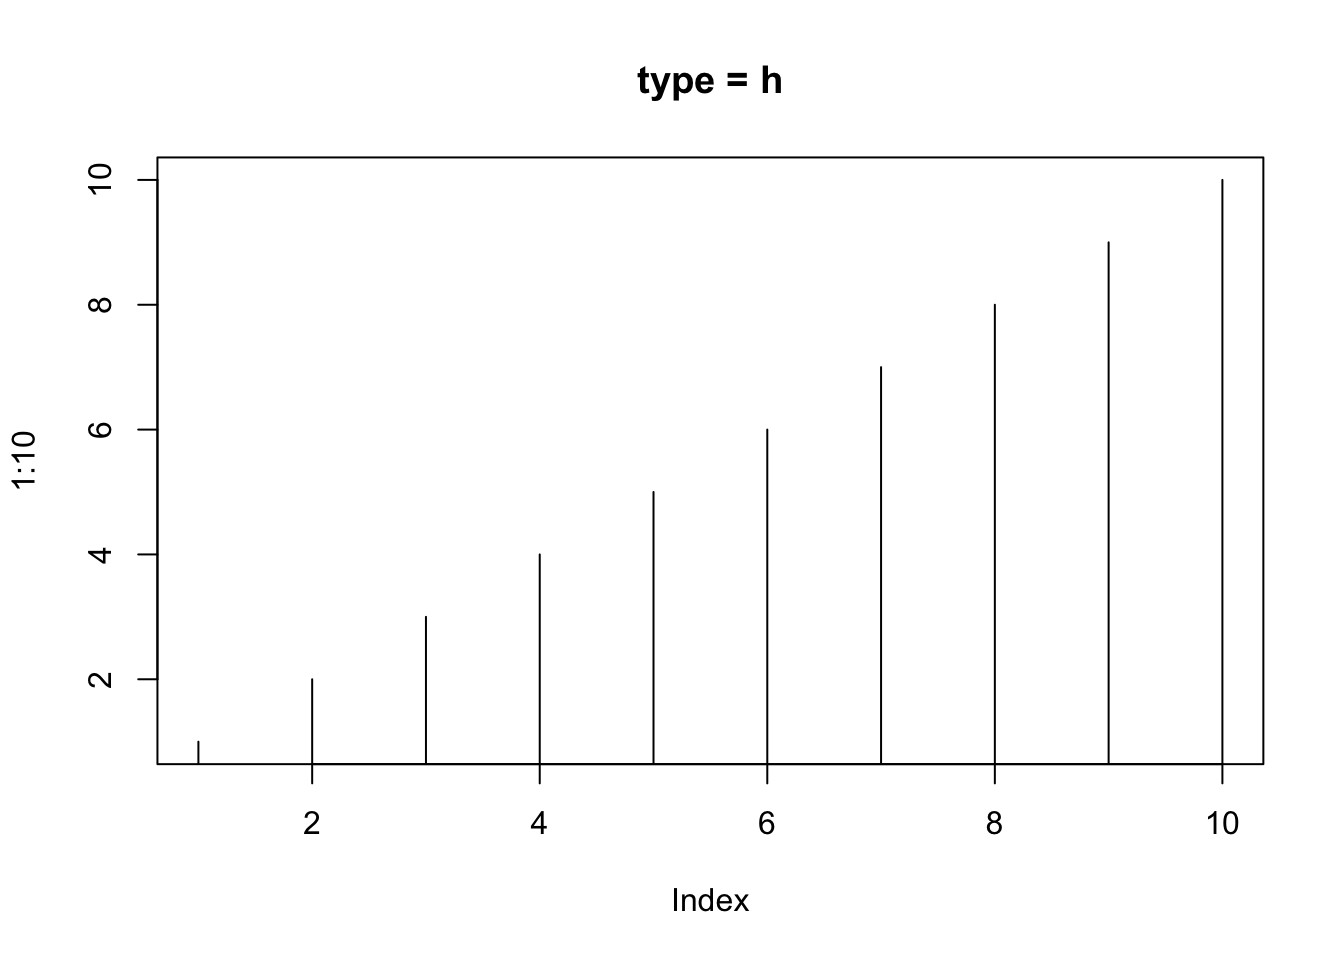
\includegraphics{Introduction-R_files/figure-latex/unnamed-chunk-77-1.pdf}

With \texttt{plot\ =\ \textquotesingle{}h\textquotesingle{}} we get a bar plot:

\begin{Shaded}
\begin{Highlighting}[]
\KeywordTok{plot}\NormalTok{ (}\DecValTok{1}\OperatorTok{:}\StringTok{ }\DecValTok{10}\NormalTok{, }\DataTypeTok{type =} \StringTok{'h'}\NormalTok{, }\DataTypeTok{main =} \StringTok{'type = h'}\NormalTok{)}
\end{Highlighting}
\end{Shaded}

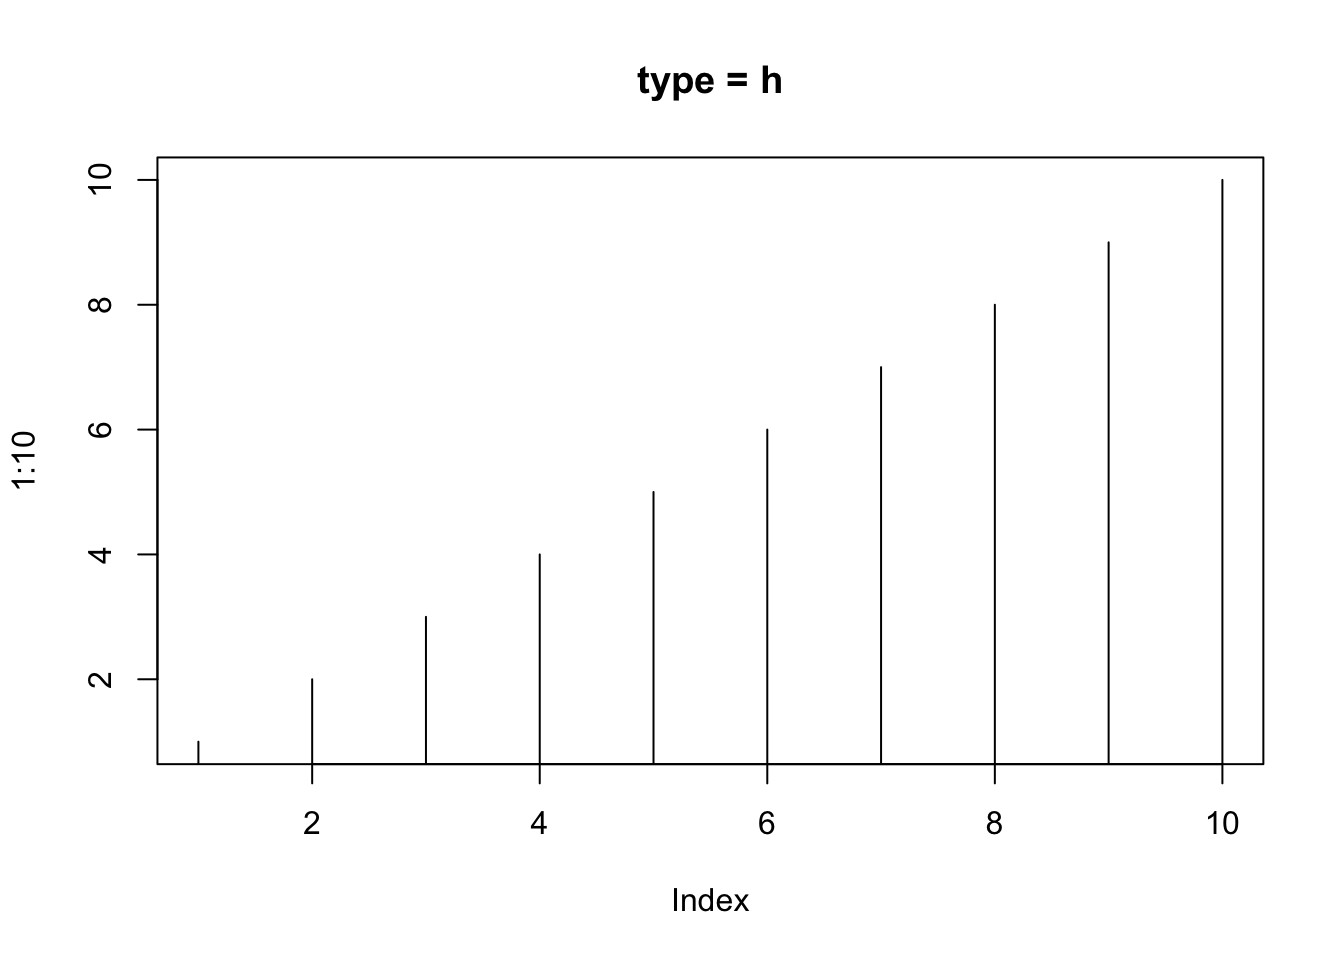
\includegraphics{Introduction-R_files/figure-latex/unnamed-chunk-78-1.pdf}

\hypertarget{graphical-parameters}{%
\section{Graphical parameters}\label{graphical-parameters}}

We have already seen that it is possible to control certain graphical elements using parameters:

\begin{longtable}[]{@{}ll@{}}
\toprule
Element & Parameter\tabularnewline
\midrule
\endhead
point & \texttt{pch}\tabularnewline
type of line graph & \texttt{type}\tabularnewline
color & \texttt{col}\tabularnewline
line & \texttt{lty},\texttt{lwd}\tabularnewline
axis label & \texttt{xlab},\texttt{ylab}\tabularnewline
axis dimensions & \texttt{xlim},\texttt{ylim}\tabularnewline
label dimensions & \texttt{cex}\tabularnewline
orientation axes labels & \texttt{las}\tabularnewline
\bottomrule
\end{longtable}

See \texttt{?par} for a description of the values that these parameters can take.

To impose parameters on all the graphics produced during a session, we will use the \texttt{par()} function. \texttt{par()} is often used to view two or more plots in the same window with the parameter \texttt{mfrow\ =\ c(l,\ c)}. In this case the graphs are displayed in a grid with \texttt{l} rows and \texttt{c} columns. Try the following:

\begin{Shaded}
\begin{Highlighting}[]
\CommentTok{# opar = par () # to be able to reset with the initial parameters}
\KeywordTok{par}\NormalTok{(}\DataTypeTok{mfrow =} \KeywordTok{c}\NormalTok{ (}\DecValTok{1}\NormalTok{,}\DecValTok{2}\NormalTok{))}
\KeywordTok{plot}\NormalTok{(wt, mpg, }\DataTypeTok{main =} \StringTok{'Weight, consumption'}\NormalTok{)}
\KeywordTok{boxplot}\NormalTok{(hp, }\DataTypeTok{main =} \StringTok{'Power'}\NormalTok{)}
\end{Highlighting}
\end{Shaded}

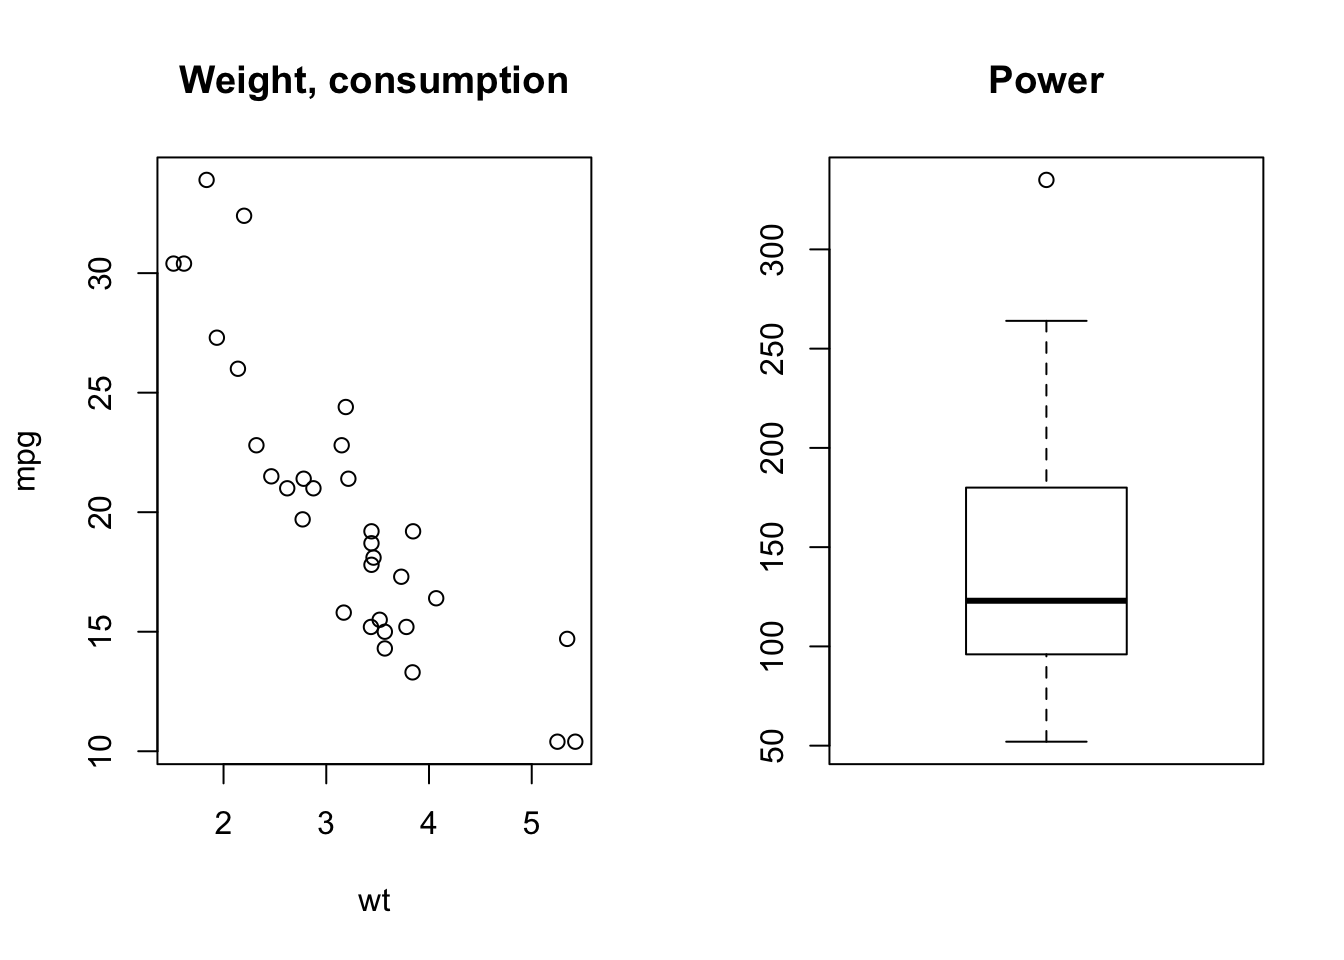
\includegraphics{Introduction-R_files/figure-latex/unnamed-chunk-79-1.pdf}

Changes are implemented until when the session is closed, or the graphics engine is reset by \texttt{dev.off()} or by clicking on the \texttt{Clear\ all\ plots} brush in \texttt{RStudio}.

\texttt{par()} is also used to change the size of the margins. This is sometimes useful when the labels on the axes do not fit in the window, as in this example:

\begin{Shaded}
\begin{Highlighting}[]
\NormalTok{mydata =}\StringTok{ }\KeywordTok{as.factor}\NormalTok{(}\KeywordTok{sample}\NormalTok{ (}\DataTypeTok{x =} \KeywordTok{c}\NormalTok{ (}\StringTok{'Paris'}\NormalTok{, }\StringTok{'London'}\NormalTok{, }\StringTok{'Brussels'}\NormalTok{, }\StringTok{'Washington'}\NormalTok{),}
                           \DataTypeTok{replace =}\NormalTok{ T,}
                           \DataTypeTok{prob =} \KeywordTok{c}\NormalTok{ (.}\DecValTok{1}\NormalTok{, }\FloatTok{.5}\NormalTok{, }\FloatTok{.2}\NormalTok{, }\FloatTok{.1}\NormalTok{),}
                           \DataTypeTok{size =} \DecValTok{100}\NormalTok{)) }\CommentTok{# simulation of a qualitative variable}
\KeywordTok{barplot}\NormalTok{(}\KeywordTok{summary}\NormalTok{ (mydata),}
        \DataTypeTok{width =} \FloatTok{.1}\NormalTok{,}
        \DataTypeTok{horiz =}\NormalTok{ T,}
        \DataTypeTok{las =} \DecValTok{2}\NormalTok{)}
\end{Highlighting}
\end{Shaded}

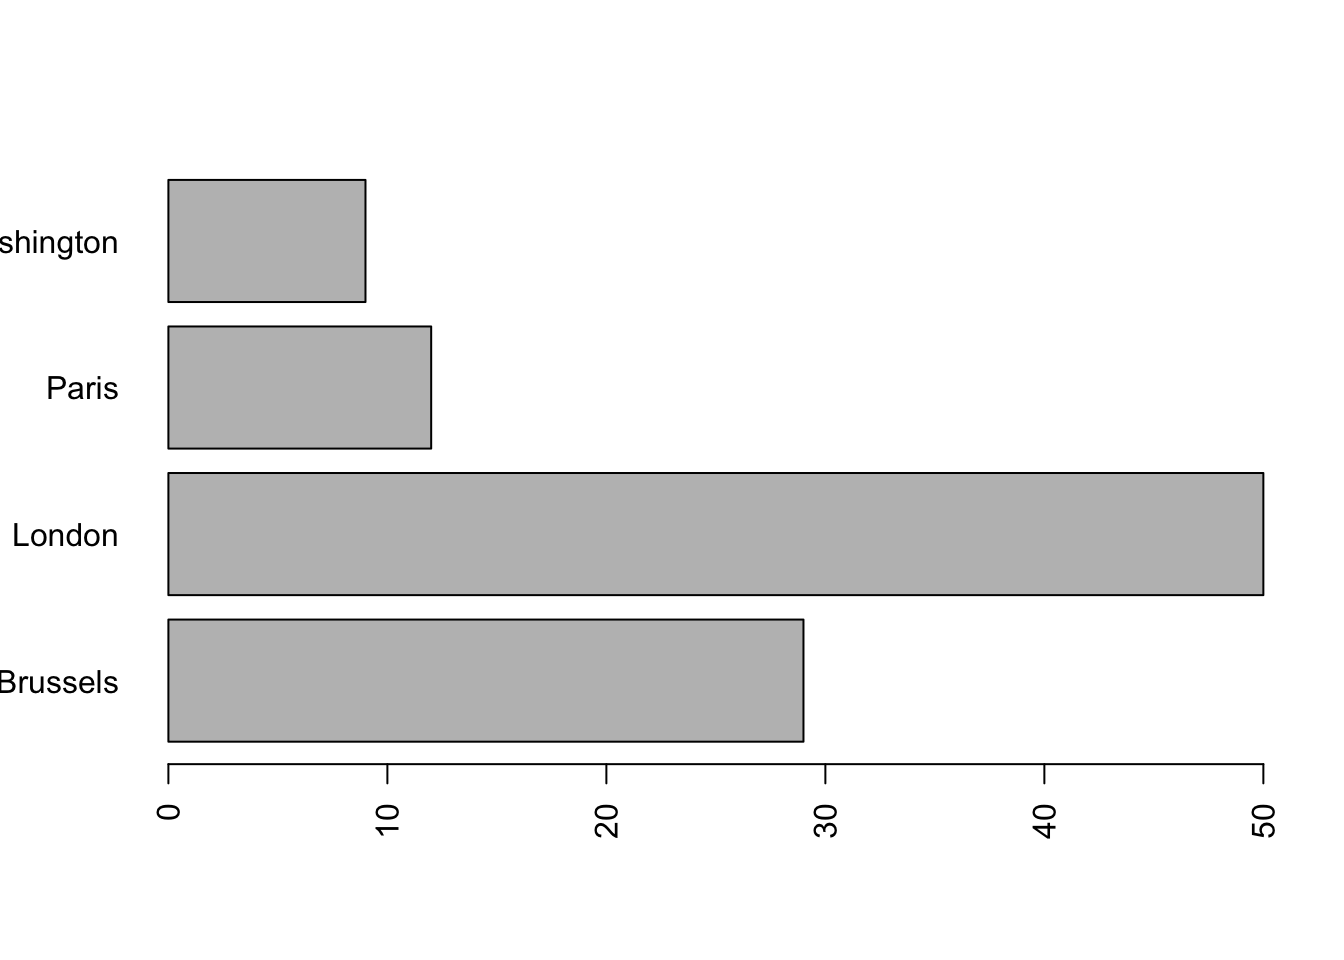
\includegraphics{Introduction-R_files/figure-latex/unnamed-chunk-80-1.pdf}

We modify the parameter which sets the left margin:

\begin{Shaded}
\begin{Highlighting}[]
\KeywordTok{par}\NormalTok{(}\DataTypeTok{mar =} \KeywordTok{c}\NormalTok{(}\DecValTok{5}\NormalTok{, }\DecValTok{6}\NormalTok{, }\DecValTok{4}\NormalTok{, }\DecValTok{2}\NormalTok{) }\OperatorTok{+}\StringTok{ }\FloatTok{0.1}\NormalTok{) }\CommentTok{# the second component of mar gives the left margin}
\CommentTok{# Default is c (5, 4, 4, 2) + 0.1}
\KeywordTok{barplot}\NormalTok{(}\KeywordTok{summary}\NormalTok{ (mydata),}
        \DataTypeTok{width =} \FloatTok{.1}\NormalTok{,}
        \DataTypeTok{horiz =}\NormalTok{ T,}
        \DataTypeTok{las =} \DecValTok{2}\NormalTok{)}
\end{Highlighting}
\end{Shaded}

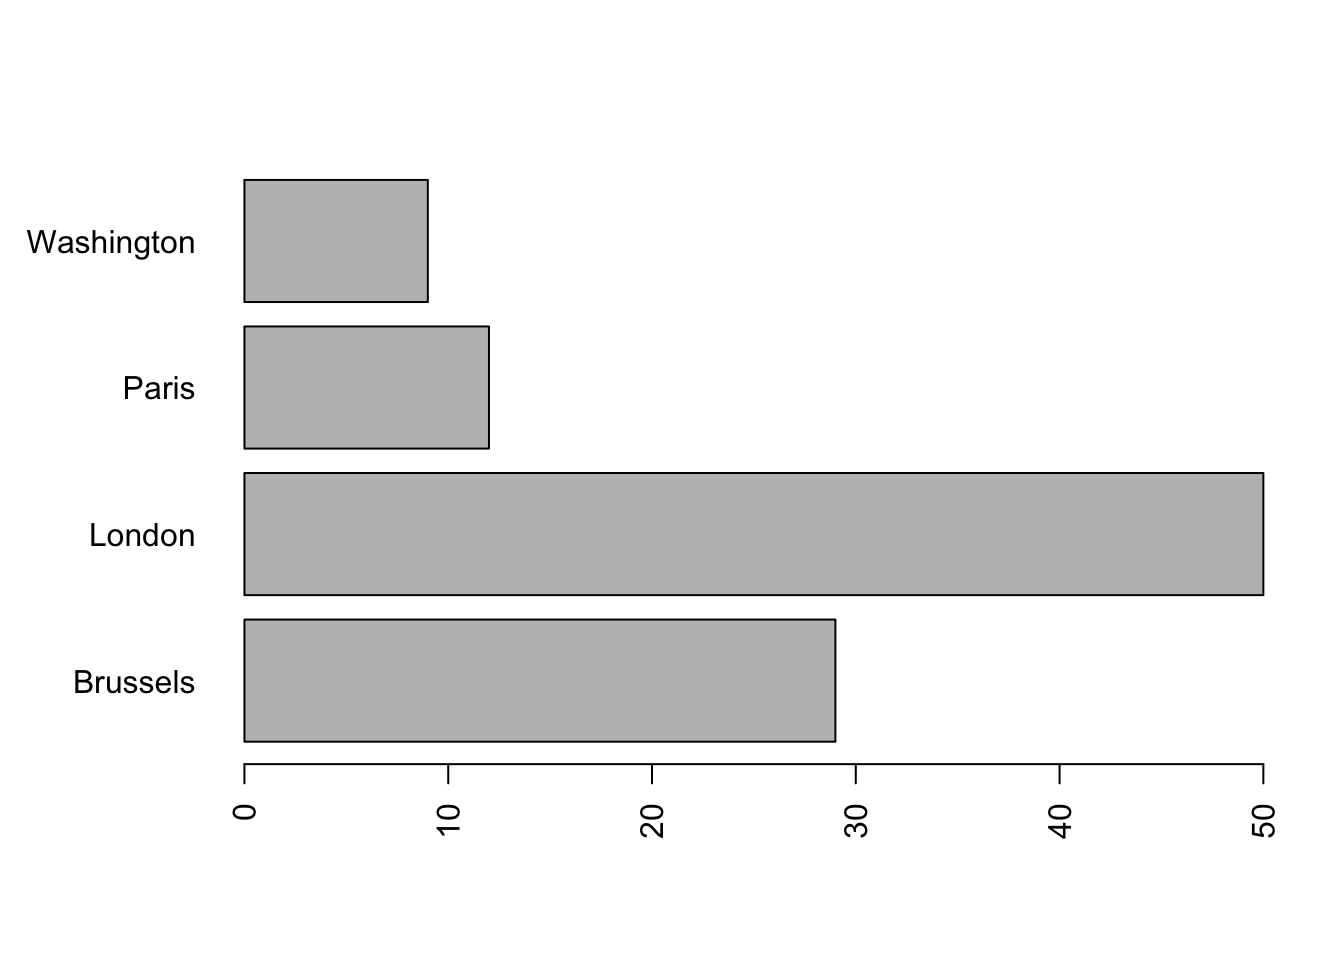
\includegraphics{Introduction-R_files/figure-latex/unnamed-chunk-81-1.pdf}

\hypertarget{histograms}{%
\section{Histograms}\label{histograms}}

As we have already noted in the subsection \ref{quant-var}, by default, \texttt{hist()} displays the histogram with the counts. To display the histogram in the density scale we use the option \texttt{freq\ =\ FALSE}. In this case, the area of each rectangle will be equal to the proportion of observations in the corresponding class (so that the total area of all the rectangles is one).

\begin{Shaded}
\begin{Highlighting}[]
\KeywordTok{par}\NormalTok{(}\DataTypeTok{mfrow =} \KeywordTok{c}\NormalTok{ (}\DecValTok{1}\NormalTok{,}\DecValTok{2}\NormalTok{))}
\KeywordTok{hist}\NormalTok{(mpg) }\CommentTok{# freq = TRUE}
\KeywordTok{hist}\NormalTok{(mpg, }\DataTypeTok{freq =} \OtherTok{FALSE}\NormalTok{)}
\end{Highlighting}
\end{Shaded}

To superimpose the curve of a given density:

\begin{Shaded}
\begin{Highlighting}[]
\NormalTok{mydata =}\StringTok{ }\KeywordTok{rnorm}\NormalTok{ (}\DecValTok{1000}\NormalTok{,}\DecValTok{0}\NormalTok{,}\DecValTok{1}\NormalTok{) }\CommentTok{# simulation of 1000 observations N (0,1)}
\KeywordTok{hist}\NormalTok{(mydata, }\DataTypeTok{freq =}\NormalTok{ F, }\DataTypeTok{main =} \StringTok{'Histogram and theoretical density'}\NormalTok{)}
\KeywordTok{curve}\NormalTok{(dnorm, }\CommentTok{# the density function of N (0,1)}
      \DataTypeTok{from =} \DecValTok{-5}\NormalTok{, }\DataTypeTok{to =} \DecValTok{5}\NormalTok{, }\CommentTok{# the range}
      \DataTypeTok{add =} \OtherTok{TRUE}\NormalTok{) }\CommentTok{# because we want to add the density of N (0,1) to the histogram}
\end{Highlighting}
\end{Shaded}

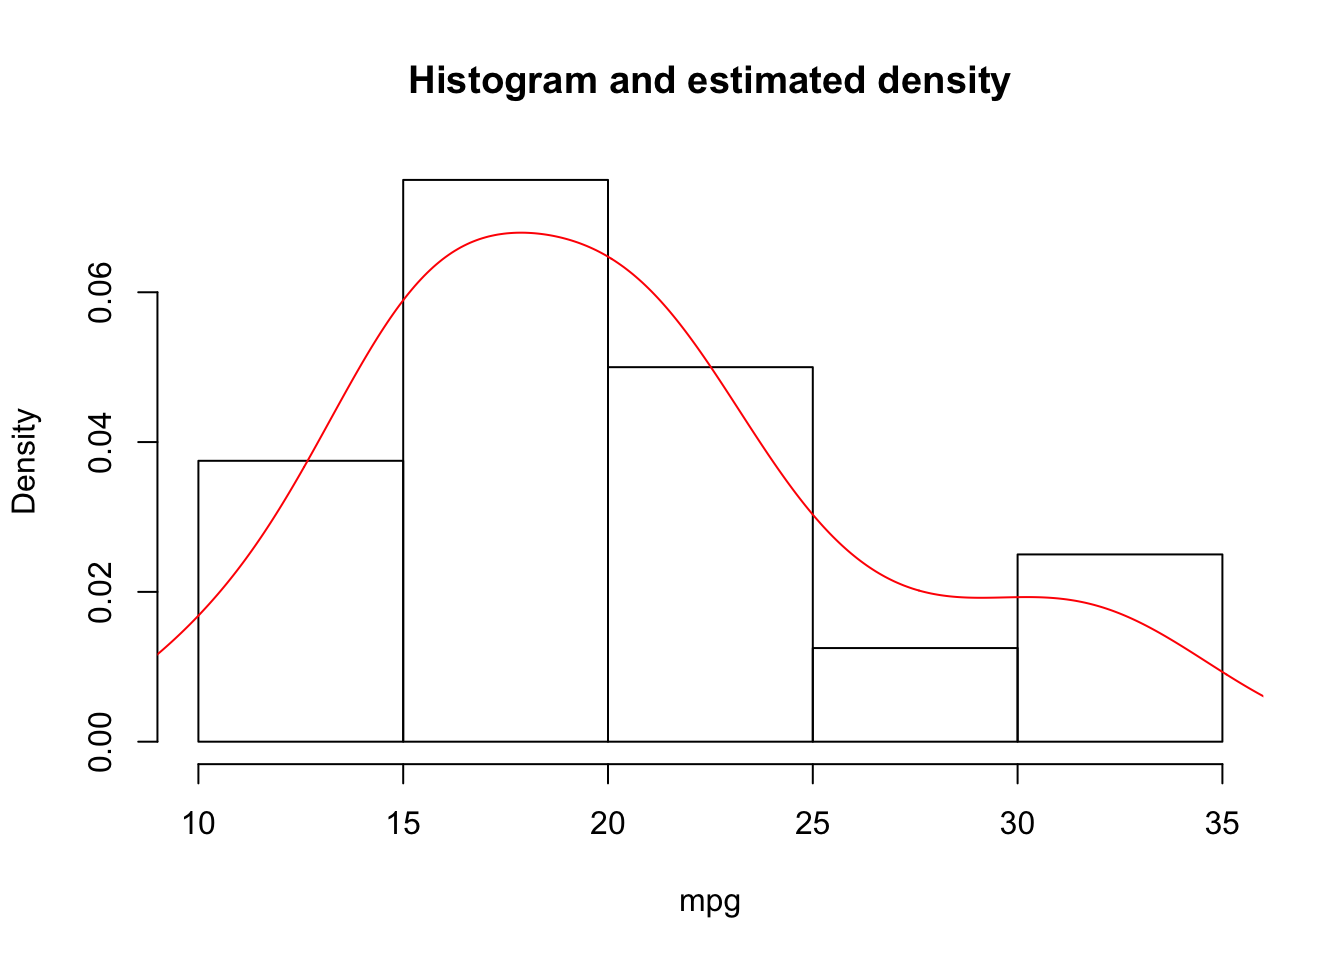
\includegraphics{Introduction-R_files/figure-latex/unnamed-chunk-83-1.pdf}

Rather than viewing the histogram of the data, we can show the estimated density (using kernel density estimation methods):

\begin{Shaded}
\begin{Highlighting}[]
\KeywordTok{hist}\NormalTok{(mpg, }\DataTypeTok{freq =}\NormalTok{ F, }\DataTypeTok{main =} \StringTok{'Histogram and estimated density'}\NormalTok{)}
\KeywordTok{lines}\NormalTok{(}\KeywordTok{density}\NormalTok{ (mpg), }\DataTypeTok{col =} \DecValTok{2}\NormalTok{)}
\end{Highlighting}
\end{Shaded}

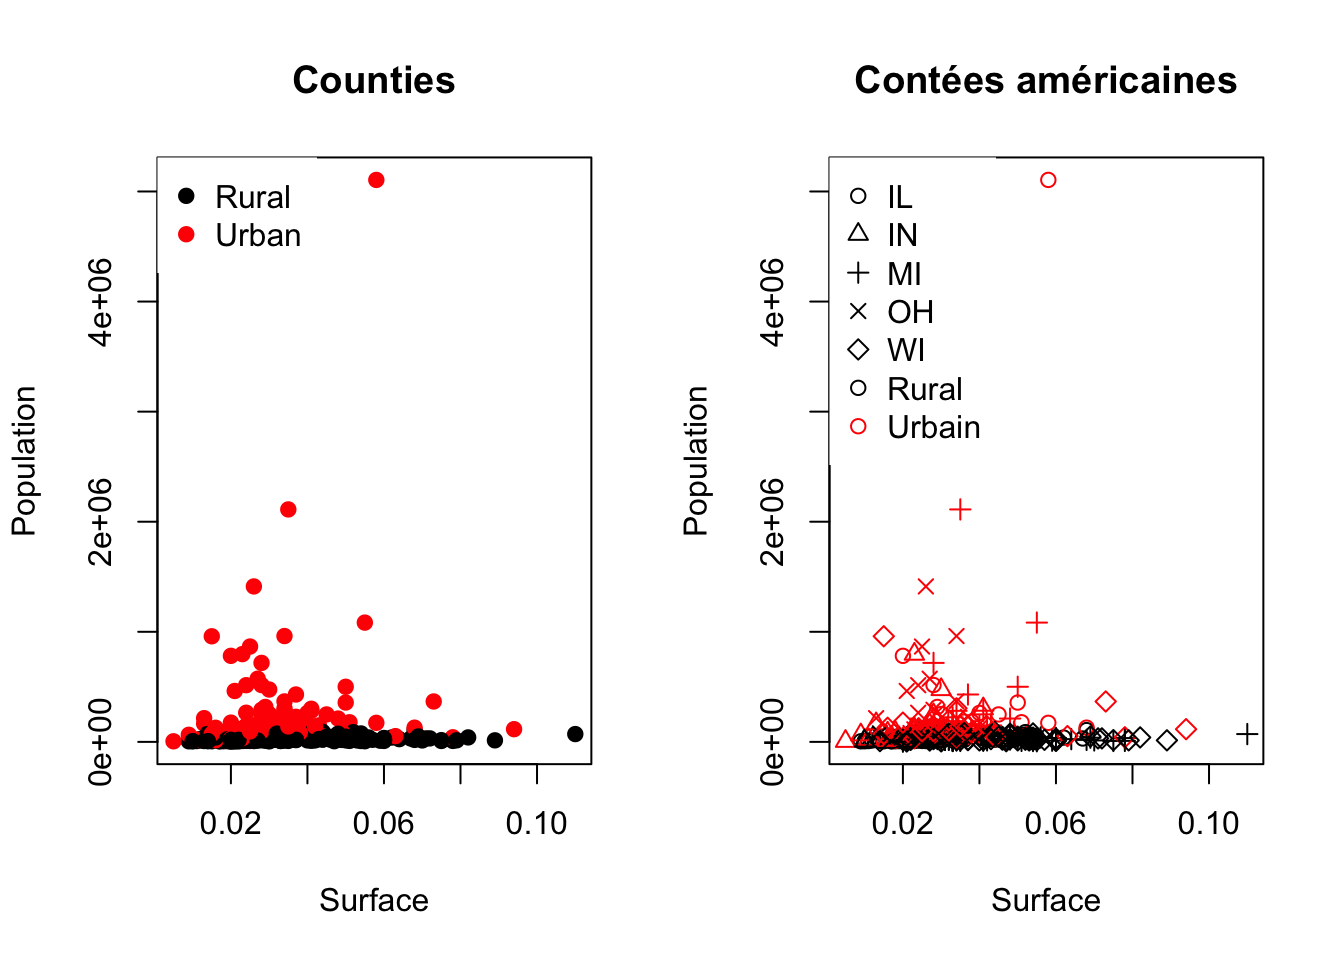
\includegraphics{Introduction-R_files/figure-latex/unnamed-chunk-84-1.pdf}

\hypertarget{exercises}{%
\section{Exercises}\label{exercises}}

\begin{enumerate}
\def\labelenumi{\arabic{enumi}.}
\tightlist
\item
  We consider the \texttt{midwest} dataset from the \texttt{ggplot2} package (an advanced graphics package).

  \begin{itemize}
  \tightlist
  \item
    Install and charge the package.
  \item
    Consult the help for the description of the variables in \texttt{midwest}.
  \item
    Reproduce the following graphics using basic functions:
  \end{itemize}
\end{enumerate}

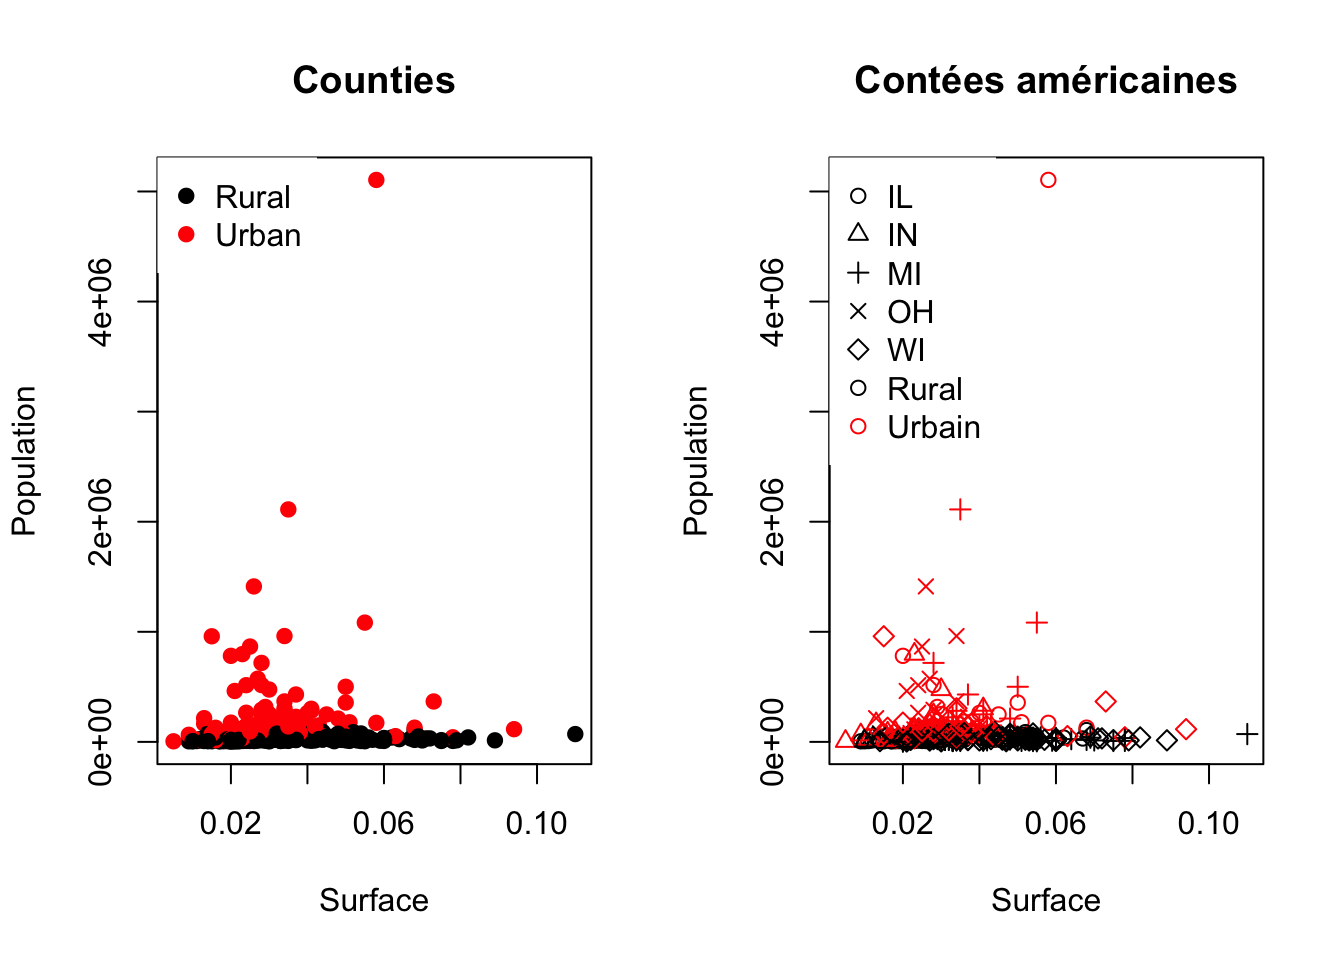
\includegraphics{Introduction-R_files/figure-latex/unnamed-chunk-85-1.pdf}

\begin{enumerate}
\def\labelenumi{\arabic{enumi}.}
\setcounter{enumi}{1}
\tightlist
\item
  We consider the \texttt{adult} dataset available on the site \href{https://archive.ics.uci.edu/ml/datasets/Adult}{archive.ics.uci.edu/ml/datasets/Adult}. The dataset consists of 48,842 rows and 14 columns.

  \begin{itemize}
  \tightlist
  \item
    Import the data into \texttt{R} from the file \texttt{adult.data}. Look in the \texttt{adult.names} file for the names of the variables.
  \item
    Describe each variable appropriately according to its type.
  \item
    Describe the relationship between the variables \texttt{age} and\texttt{class}.
  \end{itemize}
\end{enumerate}

\hypertarget{probability-distributions}{%
\chapter{Probability distributions}\label{probability-distributions}}

Let \(X\) be a random variable whose distribution is \texttt{law}:

\begin{itemize}
\tightlist
\item
  \texttt{dlaw(x,\ parameters)} computes the probability \(P(X = x)\) if \(X\) is discrete, and the density value \(f(x)\) if \(X\) is continuous with density \(f\).
\item
  \texttt{plaw(q,\ parameters)} computes the value of the Cumualative Distribution Function (CDF) in \(q\), ie \(F(q) = P(X \leq q)\).
\item
  \texttt{qlaw(p,\ parameters)} gives the quantile of order \(p\), that is the value \(q\) such that \(p = P (X \leq q)\).
\item
  \texttt{rlaw(m,\ parameters)} generates \(m\) independent random numbers according to the distribution of \(X\), ie a sample of size \(m\) of \(X\).
\end{itemize}

Consult the help with \texttt{?dlaw}.

The \texttt{set.seed()} function allows you to set the \emph{seed} of the random number generator. This is useful when you want to obtain identical simulations:

\begin{Shaded}
\begin{Highlighting}[]
\KeywordTok{runif}\NormalTok{(}\DecValTok{1}\NormalTok{) }\CommentTok{# uniform draw in [0,1]}
\end{Highlighting}
\end{Shaded}

\begin{verbatim}
## [1] 0.8366401
\end{verbatim}

\begin{Shaded}
\begin{Highlighting}[]
\KeywordTok{runif}\NormalTok{(}\DecValTok{1}\NormalTok{)}
\end{Highlighting}
\end{Shaded}

\begin{verbatim}
## [1] 0.7943818
\end{verbatim}

\begin{Shaded}
\begin{Highlighting}[]
\KeywordTok{set.seed}\NormalTok{(}\DecValTok{42}\NormalTok{); }\KeywordTok{runif}\NormalTok{ (}\DecValTok{1}\NormalTok{)}
\end{Highlighting}
\end{Shaded}

\begin{verbatim}
## [1] 0.914806
\end{verbatim}

\begin{Shaded}
\begin{Highlighting}[]
\KeywordTok{set.seed}\NormalTok{(}\DecValTok{42}\NormalTok{); }\KeywordTok{runif}\NormalTok{ (}\DecValTok{1}\NormalTok{)}
\end{Highlighting}
\end{Shaded}

\begin{verbatim}
## [1] 0.914806
\end{verbatim}

\hypertarget{discrete-distributions-of-discrete-random-variables}{%
\section{Discrete distributions of discrete random variables}\label{discrete-distributions-of-discrete-random-variables}}

Important discrete random variables are

\begin{itemize}
\tightlist
\item
  Binomial variable \(\mathcal{B}(n, p)\) counting the number of successes out of \(n\) independent trials each with probability \(p\) of success: \texttt{rbinom(m,\ size\ =\ n,\ prob\ =\ p)}. This law has \(n + 1\) distinct possible values: \(0,1,\ldots, n\).
\item
  Bernoulli variable \(\mathcal{B}(p)\) reporting the outcome of a binary trial with probability \(p\) of success: \texttt{rbinom(m,\ size\ =\ 1,\ prob\ =\ p)}
\item
  Geometric variable \(\mathcal{G}(p)\) counting the number of failures before success in independent trials: \texttt{rgeom(n,\ prob\ =\ p)}
\item
  Poisson variable \(\mathcal{P}(\lambda)\): \texttt{rpois(m,\ lambda\ =\ lambda)}
\end{itemize}

An important random process which is very useful to simulate in many situations, is the withdrawl of \(n\) balls of different colors out of a box. This can be done with

\texttt{sample(x\ =\ box,\ size\ =\ n,\ replace\ =\ TRUE\ /\ FALSE,\ prob\ =\ probability\ of\ the\ different\ colors)}

For instance:

\begin{Shaded}
\begin{Highlighting}[]
\NormalTok{x <-}\StringTok{ }\KeywordTok{c}\NormalTok{(}\StringTok{'red'}\NormalTok{, }\StringTok{'black'}\NormalTok{, }\StringTok{'green'}\NormalTok{)}
\KeywordTok{sample}\NormalTok{(}\DataTypeTok{x =}\NormalTok{ x, }\DataTypeTok{size =} \DecValTok{20}\NormalTok{, }\DataTypeTok{replace =} \OtherTok{TRUE}\NormalTok{, }\DataTypeTok{prob =} \KeywordTok{c}\NormalTok{(}\DecValTok{2}\OperatorTok{/}\DecValTok{10}\NormalTok{,}\DecValTok{4}\OperatorTok{/}\DecValTok{10}\NormalTok{,}\DecValTok{4}\OperatorTok{/}\DecValTok{10}\NormalTok{))}
\end{Highlighting}
\end{Shaded}

\begin{verbatim}
##  [1] "red"   "black" "red"   "green" "green" "green" "black" "green" "green"
## [10] "green" "green" "red"   "black" "green" "red"   "red"   "black" "green"
## [19] "green" "red"
\end{verbatim}

\hypertarget{continuous-distributions}{%
\section{Continuous distributions}\label{continuous-distributions}}

Important continuous distributions are:

\begin{itemize}
\tightlist
\item
  Uniform distribution \(\mathcal{U}_{[a, b]}\) in the interval \([a,b]\): \texttt{runif(m,\ min\ =\ a,\ max\ =\ b)}
\item
  Normal variable \(\mathcal{N}(\mu, \sigma^2)\): \texttt{rnorm(m,\ mean\ =\ mu,\ sd\ =\ sigma)}
\item
  Exponential law \(\mathcal{E}(\lambda)\): \texttt{rexp(m,\ rate\ =\ lambda)}
\item
  Chi-square law with \(r\) degrees of freedom \(\mathcal{\chi}^2 (r)\): \texttt{rchisq\ (m,\ df\ =\ r)}
\item
  Student's law with \(r\) degrees of freedom: \texttt{rt(m,\ df\ =\ r)}
\end{itemize}

\hypertarget{example-the-law-of-large-numbers}{%
\section{Example: the Law of Large Numbers}\label{example-the-law-of-large-numbers}}

We toss \(n\) times a biased coin such that the probability of getting head is \(p=0.3\) and then we calculate the proportion of heads obtained. The Law of Large Numbers says that this proportion gets closer and closer to \(p\) as \(n\) gets larger.

\begin{Shaded}
\begin{Highlighting}[]
\CommentTok{# 1: head, 0: tail}
\NormalTok{sample =}\StringTok{ }\KeywordTok{sample}\NormalTok{(}\DataTypeTok{x =} \KeywordTok{c}\NormalTok{(}\DecValTok{0}\NormalTok{,}\DecValTok{1}\NormalTok{), }\DataTypeTok{size =} \DecValTok{1000}\NormalTok{, }\DataTypeTok{replace =}\NormalTok{ T, }\DataTypeTok{prob =} \KeywordTok{c}\NormalTok{(.}\DecValTok{7}\NormalTok{, }\FloatTok{.3}\NormalTok{))}
\KeywordTok{plot}\NormalTok{(}\KeywordTok{cumsum}\NormalTok{(sample)}\OperatorTok{/}\NormalTok{(}\DecValTok{1}\OperatorTok{:}\DecValTok{1000}\NormalTok{),}
     \DataTypeTok{type =} \StringTok{'l'}\NormalTok{,}
     \DataTypeTok{main =} \StringTok{'Law of large numbers'}\NormalTok{,}
     \DataTypeTok{ylim =} \KeywordTok{c}\NormalTok{ (}\DecValTok{0}\NormalTok{,}\FloatTok{0.7}\NormalTok{),}
     \DataTypeTok{xlab =} \StringTok{'Sample size'}\NormalTok{)}
\KeywordTok{abline}\NormalTok{ (}\DataTypeTok{h =} \FloatTok{.3}\NormalTok{, }\DataTypeTok{col =} \DecValTok{2}\NormalTok{)}
\KeywordTok{legend}\NormalTok{ (}\DataTypeTok{x =} \StringTok{'top'}\NormalTok{,}
       \DataTypeTok{lty =} \DecValTok{1}\NormalTok{, }\DataTypeTok{col =} \DecValTok{1}\OperatorTok{:}\StringTok{ }\DecValTok{2}\NormalTok{,}
       \DataTypeTok{legend =} \KeywordTok{c}\NormalTok{ (}\StringTok{'empirical frequency of 1'}\NormalTok{, }\StringTok{'probability of 1'}\NormalTok{),}
       \DataTypeTok{bty =} \StringTok{'n'}\NormalTok{)}
\end{Highlighting}
\end{Shaded}

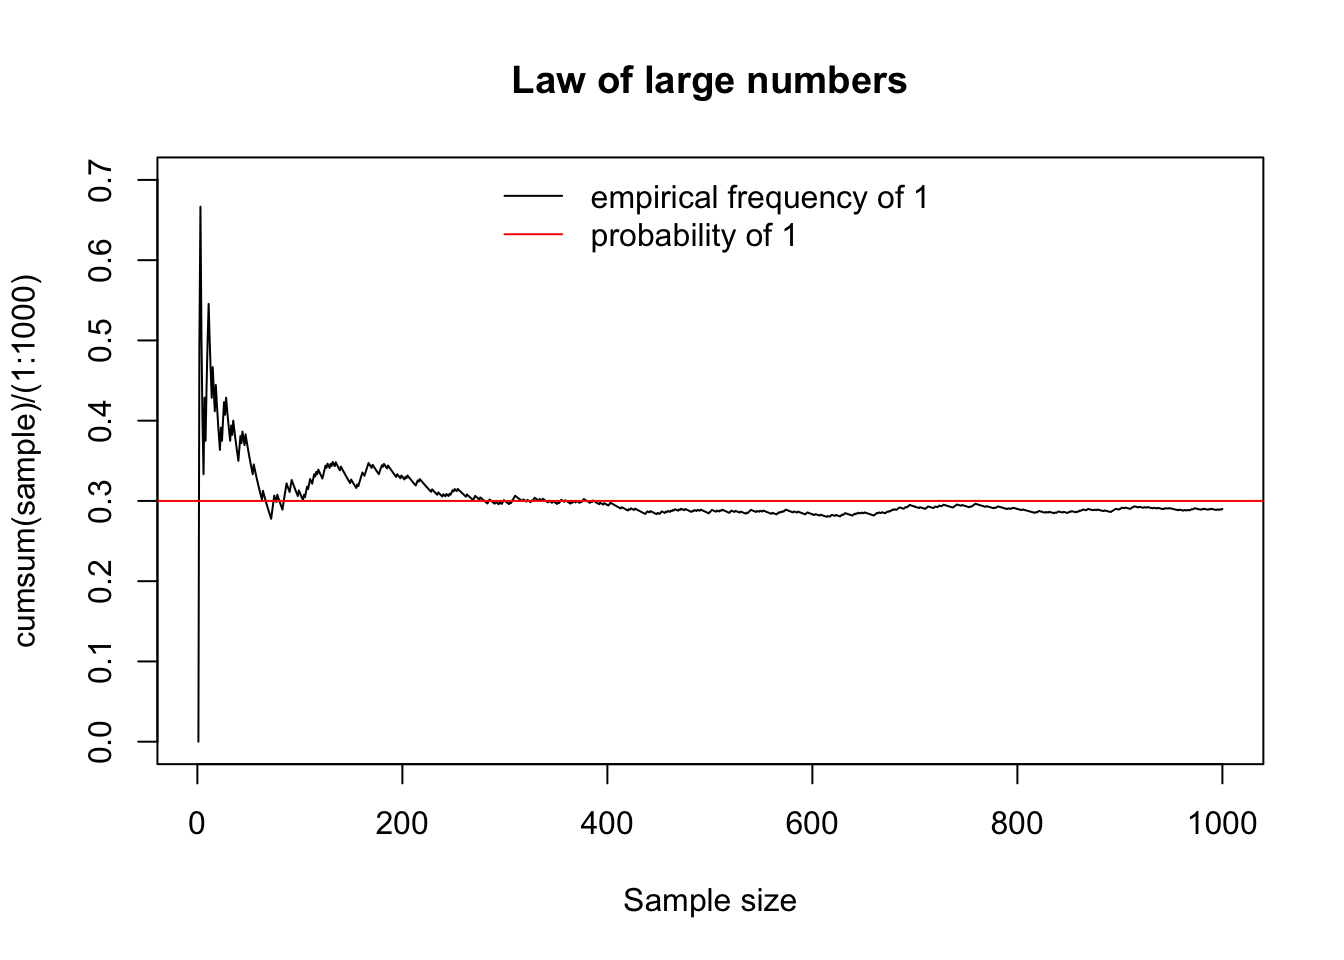
\includegraphics{Introduction-R_files/figure-latex/unnamed-chunk-88-1.pdf}

Notes:

\begin{itemize}
\tightlist
\item
  To get the number of heads as a function of \(n\) we used the \texttt{cumsum()} function. Try the following:
\end{itemize}

\begin{Shaded}
\begin{Highlighting}[]
\CommentTok{# for each n we count how many 1s there are in the first n positions:}
\KeywordTok{cumsum}\NormalTok{(}\KeywordTok{c}\NormalTok{(}\DecValTok{0}\NormalTok{,}\DecValTok{0}\NormalTok{,}\DecValTok{1}\NormalTok{,}\DecValTok{0}\NormalTok{,}\DecValTok{1}\NormalTok{,}\DecValTok{1}\NormalTok{,}\DecValTok{0}\NormalTok{)) }
\CommentTok{# for each n we calculate the proportions of 1s in the first n positions}
\KeywordTok{cumsum}\NormalTok{(}\KeywordTok{c}\NormalTok{(}\DecValTok{0}\NormalTok{,}\DecValTok{0}\NormalTok{,}\DecValTok{1}\NormalTok{,}\DecValTok{0}\NormalTok{,}\DecValTok{1}\NormalTok{,}\DecValTok{1}\NormalTok{,}\DecValTok{0}\NormalTok{))}\OperatorTok{/}\DecValTok{1}\OperatorTok{:}\DecValTok{7}
\end{Highlighting}
\end{Shaded}

\begin{itemize}
\tightlist
\item
  Instead of \texttt{sample()} we could have used \texttt{rbinom(n\ =\ 1000,\ size\ =\ 1,\ prob\ =\ .3)}
\end{itemize}

\bibliography{ref.bib}

\end{document}
